\documentclass[a4paper]{book}

\usepackage[french]{babel}
\usepackage{graphicx}
\usepackage{epsfig} % use this package to include EPS format figures
\usepackage{wrapfig}
\usepackage{amsmath}
%\usepackage[utf8]{inputenc}
\usepackage[T1]{fontenc}


%\usepackage[french]{babel}
%\usepackage[T1]{fontenc}
\usepackage{manfnt}
\usepackage{listings}
\usepackage{verbatim}
\usepackage{fancybox}
%
%\usepackage{pst-all}
%
%
\usepackage{url}
\usepackage{wrapfig}
\usepackage{titleref}
\usepackage{makeidx}
\usepackage{amsmath}
\usepackage{amsfonts}
\usepackage{amssymb}
\usepackage{quotchap}
\usepackage{xcolor}
\usepackage{lmodern}
\usepackage{microtype}

%Chapitre sans numero, avec ajout automatique dans la TOC
\newcommand{\starlesschapter}[1]
{
    \chapter*{#1}
    \addcontentsline{toc}{chapter}{#1}
    \markboth{ \MakeUppercase{#1} }{ \MakeUppercase{#1} }
}

\newcommand{\includecodecaption}[2]{%
\begin{DDbox}{\linewidth}%
\lstinputlisting[caption = #2, label=lst:#1]{../../code/#1}%
\end{DDbox}%
}

%Environnement de recapitulatif
\newcommand{\titledframe}[2]{%
\boxput*(-0.6,1){\psframebox*{#1}}%
{\psshadowbox[framesep=12pt]{#2}}}%

\newenvironment{recapitulatif}%
{%
\newpage
\begin{Sbox}%
\begin{minipage}{\textwidth}%
\medskip%
 \begin{list}%
    {$\bullet$}%
    {\setlength{\labelwidth}{30pt}%
     \setlength{\leftmargin}{35pt}%
     \setlength{\itemsep}{\parsep}}%
}
{\end{list} \end{minipage}\end{Sbox}%
\medskip%
%\titledframe{\normalfont{\Large{\bfseries{Récapitulatif}}}}{\TheSbox}%
}%

%Environnement bonnes habitudes
\newcommand{\titledframehabitudes}[2]{%
\boxput*(-0.6,1){\psframebox*{#1}}%
{\psframebox[framesep=12pt]{#2}}}%


\newenvironment{habitudes}%
{%
\begin{floatingfigure}{5cm}
\begin{Sbox}%
\begin{minipage}{4.5cm}%

}
{ \end{minipage}\end{Sbox}%
\medskip%
\titledframehabitudes{\normalfont{{\bfseries{Bonnes habitudes}}}}{\TheSbox}%
\end{floatingfigure}
}%

\newtheorem{habit}{Bonnes habitudes}

\renewenvironment{habitudes}
{%
\begin{habit}
}
{
\end{habit}
}

%Mots cles, fonctions et autres classes en C++
\newcommand{\keyword}[1]{%
\texttt{#1}%
}

\newcommand{\classname}[1]{%
\texttt{#1}%
}

\newcommand{\functionname}[1]{%
\texttt{#1}%
}

\newcommand{\varname}[1]{%
\texttt{#1}%
}

%inclusion d'un fichier de code, avec titre automatique
\newcommand{\includecode}[1]{%
\begin{DDbox}{\linewidth}%
\lstinputlisting[caption = #1, label=lst:#1]{../../code/#1}%
\end{DDbox}%
}

%inclusion d'un fichier de code, avec titre automatique
\newcommand{\includecodeWithLabel}[1]{%
\begin{DDbox}{\linewidth}%
\lstinputlisting[caption = #1, label=lst:#1]{../../code/#1}%
\end{DDbox}%
}

\def\warning{\marginpar{\dbend}}

\newenvironment{warning2}
{
\begin{DDbox}{\linewidth}%
\marginpar{\dbend}
}
{
\end{DDbox}%
}

%%configuration de listings
\lstset{
language=c++,
basicstyle=\ttfamily\small, %
identifierstyle=\color{black!60}, %
keywordstyle=\color{blue}, %
stringstyle=\color{red}, %
commentstyle=\it\color{green!95!yellow!1}, %
columns=flexible, %
tabsize=2, %
extendedchars=true, %
showspaces=false, %
showstringspaces=false, %
numbers=left, %
numberstyle=\tiny, %
breaklines=true, %
breakautoindent=true, %
captionpos=b
}

\definecolor{Zgris}{rgb}{0.87,0.85,0.85}

\newsavebox{\BBbox}
\newenvironment{DDbox}[1]{
\begin{lrbox}{\BBbox}\begin{minipage}{\linewidth}}
{\end{minipage}\end{lrbox}\noindent\colorbox{Zgris}{\usebox{\BBbox}} \\
[.5cm]}

\begin{document}

\input{../FirstPage/firstpage}

\chapter{Note pr\'eliminaire}
Ces notes de cours ne constituent qu'une version pr\'eliminaire d'un cours toujours en \'ecriture. Elles sont amen\'ees \`a \'evoluer et \`a \^etre modifi\'ees,
plus particuli\`erement en fonction des retours des \'el\`eves et relecteurs. Tout commentaire, agr\'eable ou non, est le bienvenu.


\chapter*{Remerciements}
Je souhaiterais remercier tous ceux qui m'ont aid\'e, de pr\`es ou de loin, lors de l'\'ecriture de ce cours. David Siba\"{\i} tout d'abord, qui avait entam\'e les premiers chapitres de ce polycopi\'e quand il \'etait assistant informatique \`{a} l'ENSAE, et sans qui je ne me serais probablement pas lanc\'e dans cette r\'edaction. Xavier Dupr\'e, Pierre Jacob, J\'er\'emie Jabukowicz, et David encore, pour toutes nos discussions au Gentleman ou ailleurs. J\'er\'emie Bonnefoy, pour ses relectures attentives. Les \'etudiants de ce cours depuis 2009, pour leur int\'er\^{e}t, leurs questions, remarques, ou reproches. Ma femme Elodie, pour avoir support\'e la r\'edaction en parall\`{e}le de ce document et de mon manuscrit de th\`{e}se.

\begin{quote}

\end{quote}

\tableofcontents

\begin{savequote}[65mm]
--- It looked like a good thing to do.
\qauthor{Dennis Ritchie, \`a propos de l'invention du langage C}

--- The more general aim was to design a language in which I could write
programs that were both efficient and elegant.
Many languages force you to choose between those two alternatives.
\qauthor{Bjarne Stroustrup, \`a propos de l'invention du langage C++}
\end{savequote}

\chapter{Notes sur le C++}
\bigskip

Le langage C est apparu au cours de l'ann�e 1972 dans les Laboratoires Bell. Il
fut d�velopp� en m�me temps qu'UNIX par Dennis Ritchie et Ken Thompson.
L'objectif \'etait d'\'ecrire un langage de programmation permettant le
d\'eveloppement rapide de syst\`emes d'exploitation (OS). Dennis Ritchie fit �voluer
un langage existant --le langage B-- dans une nouvelle version suffisamment
diff�rente pour qu'elle soit appel�e C. Le succ\`es du C fut rapide, en raison
de sa portabilit\'e\footnote{C'est-\`a-dire la possibilit\'e d'utiliser un programme tap\'e sur un ordinateur donn\'e et un syst\`eme d'exploitation donn\'e sur un autre ordinateur et un autre syst\`eme d'exploitation.} et des performances du code �crit.\\

Dix ans plus tard, Bjarne Stroustrup, int\'eress\'e par la programmation
orient\'ee objet qui commen�ait \`a se r\'epandre chez les universitaires,
d�veloppa le langage C++, successeur du C, alors qu'il travaillait dans le
laboratoire de recherche Bell d'AT\&T. Il s'agissait en l'occurrence
d'am�liorer le langage C en lui ajoutant une composante objet (le C++ s'appelait alors C with classes). La proximit\'e
du C++ avec le C, coupl\'ee aux facilit\'es qu'il offrait firent qu'il fut
rapidement adopt\'e.\\

Le C++ a �t� largement adopt� par la communaut� des d�veloppeurs et peut �tre consid�r� comme
le langage de r�f�rence des ann�es 80 et 90. Dans les ann�es 2000, des langages plus faciles\footnote{tout est question de point de vue �videmment} mais aux performances comparables (Java et C\# par exemple) sont pr�f�r�s pour le d�veloppement de nouveaux projets. Cependant, le C++ reste le langage de r�f�rence : de tr�s nombreux projets d�but�s dans les ann�es 80/90 ont �t� cod�s en C++ et n'ont pas �t� port�s vers des langages plus r�cents. En finance par exemple, il reste le langage le plus utilis� aujourd'hui (2012) car de tr�s nombreuses biblioth�ques toujours en production ont �t� d�velopp�es en C++, m�me si les nouveaux projets ont tendance � regarder du c�t� de langages plus r�cents, objets ou fonctionnels. Plus proche de la machine que les langages plus r�cents, le C++ permet au prix d'une complexit� plus forte un meilleur contr�le sur la machine et donc sur les performances\footnote{sous condition d'une excellente ma�trise du langage}.\\

Le C++ est un langage multi-paradigme, pouvant � la fois �tre proc�dural \footnote{Plus par souci de compatibilit� avec le C qu'autre chose d'ailleurs, je vous conseille vivement de ne pas coder en proc�dural...} et orient� objet, permettant de la programmation g�n�rique tr�s pouss�e (jusqu'au template m�ta-programming en fait), mais aussi un d�but de programmation fonctionelle. Le C++ est un langage particuli�rement difficile, suffisamment proche du langage machine pour que nous ayons besoin parfois de connaissances hardwares pour optimiser notre code, mais aussi suffisamment abstrait pour exprimer une r�elle complexit� dans les concepts manipul�s.\\ 

Enfin, comme nous le verrons dans ce polycopi�, le C++ est un langage b�tard. Pour qu'un langage soit coh�rent, il est n�cessaire que le principal de ses concepts clefs soit d�fini d�s sa cr�ation, qu'une vision � long terme du langage soit explicit�e d�s le d�part. Le C++ est n� � une p�riode o� de nombreux concepts informatiques �mergeaient. Construit "par dessus" le C, il reprend l'int�gralit� de la spec du C (pour convaincre les d�veloppeurs C de passer sous C++) et a ajout� au fur et � mesure de l'avancement des concepts, des couches suppl�mentaires au langage. L'enrichissement de ces concepts a men� � une sorte d'hydre, un langage puissant mais peu structur� qui s'est d�velopp� dans de nombreuses voies diff�rentes. C'est donc � la fois un langage de r�f�rence et d'exp�rimentation.\\

\textit{A qui s'adresse le C++ ? Pourquoi enseigner et utiliser le C++ aujourd'hui ?}\\

Le C++ est un langage tr�s performant en vitesse d'execution (surtout lorsqu'il n'abuse pas des concepts introduits entre le C et le C++), particuli�rement adapt� � la cr�ation de biblioth�ques scientifiques ou d'applications temps r�els comme dans le cadre de radars, de contr�leur de tableaux de bord dans les avions, de trading tr�s haute fr�quence, etc.\\

Cette haute performance a un prix : le C++ est un langage complexe, laborieux, peu adapt� pour de nombreuses choses naturelles dans des langages plus r�cents comme le d�veloppement web par exemple. En dehors d'un contexte avec des contraintes �normes sur la performance, tr�s peu de projets informatiques ambitieux ont donc de raisons valables de se lancer aujourd'hui dans ce langage.\\

L'int�r�t p�dagogique du C++ est soumis � d�bat : d'un c�t�, il est suffisamment difficile pour forcer l'�tudiant � assimiler de nombreux concepts qu'il serait possible de contourner dans d'autres langages. De l'autre, il est actuellement souvent un mauvais choix de technologie pour monter un projet logiciel. En raison des contraintes industrielles actuelles, les jeunes dipl�m�s de l'ENSAE se trouvent cependant amen�s � travailler sur du code en C++, ou sur des langages pour lesquels la transition est assez ais�e (notamment le Java et le C\#). C'est pour cette raison que l'enseignement � l'ENSAE reste pour quelques ann�es encore en C++. J'invite cependant les �tudiants d�sireux de monter un ambitieux projet logiciel � pr�f�rer un des langages plus r�cents pr�c�demment cit�s.\\

Ce document est la version �crite du cours d'introduction au C++ dispens� � l'ENSAE. Dans le cas de l'informatique, il est difficile de proposer le m�me contenu en cours magistral et dans un polycopi�. La syntaxe du C++ ou la compilation peuvent �tre rapidement expliqu�es � l'oral par l'exemple, alors que la m�me explication dans ce document prend n�cessairement des volumes plus consid�rables. Ceci a pour cons�quence que les d�tails et les contraintes techniques ont m�caniquement dans ce document une place relative plus importante qu'en cours. C'est malheureusement au prix d'une place relative plus faible pour les concepts de programmation objet qui me semblent bien plus fondamentaux que la syntaxe du langage par exemple.\\

J'ai choisi d'�crire ce document en d�pit de l'existence de centaines de documents similaires, disponibles en livres imprim�s ou sur le web. A mes yeux, trop de ces documents n'�taient pas adapt�s � l'enseignement du C++ pour des ing�nieurs. En effet, il existe effectivement des "bibles", comme les ouvrages de Stourstrup \cite{CppIntro} ou \cite{Thinking}, tr�s compl�tes et techniques, mais qui s'adressent � des lecteurs d�ja familiers avec la programmation, ou alors des livres
de "vulgarisation" trop peu ambitieux pour des ing�nieurs. Avec ce document, j'esp�re fournir un cours qui soit adapt� � la fois � vos attentes, mais aussi � votre vitesse de compr�hension.\\

Dans la mesure du possible, j'ai consenti � de multiples ellipses dans les premiers chapitres, prenant le risque d'�tre impr�cis, afin d'aller au plus vite au coeur du langage. Ces ellipses volontaires sont aussi un moyen de d�poussi�rer l'apprentissage du C++ en choisissant de ne pas expliquer les concepts du C pr�sents dans le C++ mais qui n'ont plus beaucoup de sens aujourd'hui; certains sont discutables ( je ne traiterai pas des structures), d'autres sont plus consensuels.\\

J'ai pris le parti d'organiser ce cours en deux grandes parties qui filent la m�taphore des langues vivantes: je pr�sente dans une premi�re grande partie la grammaire et l'orthographe du C++. La deuxi�me partie, de loin la plus importante et sur laquelle vous serez jug�s, sera celle du style. Il s'agit dans cette deuxi�me partie de comprendre comment architecturer votre code, de comprendre pourquoi certains designs sont bien sup�rieurs � d'autres.\\

Enfin, un langage de programmation ne s'apprend que d'une seule mani\`ere : par
la \emph{pratique}. R\'ep\'etons-le : sans \'ecrire de programme, il n'est pas
possible de ma\^itriser un langage. Pour ce faire, des Travaux Dirig\'es, avec
un corrig\'e d\'etaill\'e vous sont fournis sur le wiki de l'�cole (Pamplemousse).


\begin{savequote}[65mm]
--- A novice was trying to fix a broken Lisp machine by turning the power off and on. Knight, seeing what the student was doing spoke sternly: "You cannot fix a machine just by power-cycling it with no understanding of what is going wrong." Knight turned the machine off and on. The machine worked.
\qauthor{In \cite{AMP}, from "Al Koans", a collection of jokes popular at MIT in the 1980s}
\end{savequote}

\chapter{Quelques notions hardware}
\label{chapter:hardware}

\begin{center}
\textit{Ce chapitre peut �tre omis en premi�re lecture.}
\end{center}

Ce chapitre a pour vocation de fournir une tr�s br�ve introduction aux diff�rents composants d'un ordinateur commercial. Au fur et � mesure des progr�s de l'informatique, le d�veloppement logiciel a �t� suffisamment abstrait du hardware sur lequel les programmes �taient ex�cut�s pour qu'il soit possible de d�velopper une application sans connaissances particuli�res sur les machines ex�cutant le code. Cependant, les applications intensives en "calcul" impliquent une utilisation efficace du hardware qui proc�de directement des connaissances du d�veloppeur; les abstractions d�velopp�es se r�v�lant souvent insuffisantes pour g�rer de mani�re performante le hardware dans les cas critiques.\\

Depuis 30 ans, les progr�s technologiques en terme de hardware ont �t� tels qu'il faut donc d�sormais des ann�es pour acqu�rir une connaissance satisfaisante sur le fonctionnement d'un simple ordinateur classique. C'est bien �videmment tr�s au-del� de l'ambition de ce cours, mais certains points seront abord�s dans le cours avanc� dispens� en troisi�me ann�e. Nous renvoyons le lecteur curieux � une introduction en la mati�re tr�s technique mais accessible aux plus motiv�s : \cite{Drepper}. Dans ce chapitre, nous ne donnons donc qu'un aper�u des diff�rents composants d'une machine classique afin de donner quelques id�es �l�mentaires.\\

On peut d�finir la naissance des premiers ordinateurs (plut�t calculatrices g�antes) dans les ann�es 40, avec l'�quipe Von Neumann. Pour les besoins en calculs du projet Manhattan � Los Alamos, Von Neumann �labore avec Mauchly et Eckert en s'inspirant des travaux de Turing\footnote{Alan Turing est avec Von Neumann l'un des p�res de l'informatique. Il s'est suicid� en croquant une pomme empoisonn�e au cyanure, probablement en r�f�rence � Blanche-Neige; le logo d'Apple est un hommage � Turing.} un premier calculateur, dont le design est depuis appel� (plut�t injustement) architecture de Von Neumann. C'est cette architecture qui reste pr�sente dans la quasi-totalit� des architectures actuelles \footnote{m�me si l'architecture interne des micro-processeurs depuis 10 ans s'en �carte continuellement}. Dans ces premiers ordinateurs, la machine avait tr�s principalement vocation au calcul. Chacun des composants �tait fabriqu� sp�cifiquement pour cette machine, par le m�me constructeur.\\

Ce n'est plus aujourd'hui le cas : les diff�rents constructeurs de CPU, de RAM ou de cartes graphiques sont des soci�t�s distinctes. Pour donner quelques exemples, les constructeurs CPU comptent des soci�t�s comme Intel, AMD, etc.; les constructeurs RAM sont repr�sent�s par exemple par Samsung, Toshiba, Rambus, etc.; les constructeurs de carte graphique sont principalement Nvidia et ATI. Le r�sultat de cette sp�cialisation des constructeurs dans certains composants est qu'� la diff�rence des premiers ordinateurs, certains des composants d'un ordinateur vont �tre tr�s rapides par rapport aux autres, et ce seront les composants les plus lents qui ralentiront souvent la machine.\\

\section{Le CPU}

Le CPU (Central Processing Unit) est le composant principal de calcul. Les CPU qui nous int�ressent sont construits sur un seul circuit imprim� (depuis les ann�es 1970) : on les appelle micro-processeurs. Un CPU moderne est constitu� de millions de transistors, qui permettent de r�aliser de tr�s nombreuses op�rations math�matiques par seconde.\\

Depuis une dizaine d'ann�es, les processeurs sont progressivement devenus multi-coeurs, c'est � dire qu'ils contiennent chacun plusieurs entit�s de calcul appel�es coeurs. L'organisation et la r�partition des calculs sur ces diff�rents coeurs est laiss�e � la charge des d�veloppeurs et du syst�me d'exploitation (OS, pour Operating System).\\

Sur les CPUs modernes\footnote{hormi partiellement pour certaines consoles de jeux}, les diff�rents composants internes de chaque coeur sont synchronis�s sur une sorte d'horloge. A chaque modification de l'�tat interne du coeur, chacun des composants peut se retrouver dans un �tat �lectrique diff�rent, et il importe que chacun de ces composants internes soit stabilis� (au sens �lectrique du terme) avant de "regarder" � nouveau le coeur. L'horloge fournit un m�canisme de synchronisation en fournissant des "ticks" r�guliers. A chaque tick, chacun des composants a eu le temps de se stabiliser (fin du r�gime transitoire) et le coeur se trouve donc dans un �tat global coh�rent. On voit donc que la performance d'un coeur va d�pendre de la dur�e du r�gime transitoire entre deux �tats, mesur�e par la dur�e entre deux ticks de l'horloge. Cette performance est donc mesur�e en une fr�quence, qui d�crit le nombre de cycles d'horloge par seconde que peut r�aliser le coeur. Actuellement, les processeurs modernes ont des coeurs qui tournent autour de 3 GHz, c'est � dire que chaque coeur r�alise un peu plus de 3 milliards de cycles d'horloge par seconde. \\

Les composants internes principaux d'un CPU sont :

\begin{enumerate}
\item \textit{l'unit� arithm�tique et logique (UAL, ou ALU en anglais)}, qui prend en charge les calculs arithm�tiques et les tests logiques (comme les branchements IF).
\item \textit{les registres}, qui sont des m�moires de tr�s petite taille (quelques octets) et en tr�s petit nombre. Ils sont cependant tr�s rapides, et l'UAL peut les manipuler comme elle l'entend � chaque cycle d'horloge.
\item \textit{L'horloge}, qui fournit un m�canisme de synchronisation interne des diff�rents composants.
\item \textit{L'unit� de contr�le}, qui utilise l'impulsion fournie par l'horloge pour synchroniser les diff�rents composants.
\item \textit{L'unit� d'entr�e-sortie}, qui g�re les communications avec les p�riph�riques, ext�rieurs au CPU (RAM, carte graphique, �cran, souris, clavier, disque dur, imprimante, ports USB, etc.).
\end{enumerate}

Sur chaque coeur, nous pouvons faire une op�ration (multiplication ou addition) par cycle d'horloge\footnote{Sur les processeurs hyper-thread�s, on peut en fait faire une multiplication ET une addition par cycle d'horloge}, c'est � dire jusqu'� pr�s de 3 milliards d'op�rations sur des nombres r�els par seconde (3 GFlops).\\

\section{La m�moire}

La m�moire d'un ordinateur est r�partie sur de multiples composants. Tous les composants d'un ordinateur stockent des donn�es, au moins celles n�cessaires � leur fonctionnement instantan�. Certains composants (m�moire RAM, m�moire Cache, disque-dur) sont cependant enti�rement d�di�s � stocker les donn�es et � les rendre disponibles pour les autres �l�ments. Ces composants de stockage se distinguent suivant trois crit�res : la persistence ou non des donn�es lorsque la machine est �teinte/rallum�e, la vitesse d'acc�s aux donn�es stock�es, et la capacit� de stockage.\\

\subsection{Disque dur (Hard disk drive : HDD)}

Le disque dur est un syst�me de stockage massif de donn�es mais au d�bit relativement faible. Un disque dur commercial peut actuellement stocker plusieurs T�raoctet (To), c'est � dire mille Gigaoctets (Go). Le disque dur fournit un syst�me de stockage dans lequel les donn�es sont persist�es apr�s l'extinction de la machine. C'est sur le disque dur que sont stock�es toutes vos donn�es personnelles, les donn�es de vos programmes, les donn�es du syst�me d'explotation, etc.\\

Le principal probl�me actuel des disques durs est la vitesse avec laquelle les donn�es peuvent �tre lues et �crites. En effet, les disques-durs actuels\footnote{La techno est en train d'�tre remplac�e par des SSD mais devrait �tre encore dominante pour quelques ann�es.} reposent sur un syst�me de stockage magn�tique sur des disques empil�s les uns sur les autres. Tout comme pour les vieux lecteurs de disque 33 et 45 tours, des t�tes de lecture se d�placent autour du disque pour aller lire les donn�es\footnote{c'est souvent un des composants les plus fragiles: lorsque vous faites tomber votre laptop, les t�tes de lecture viennent souvent perforer les disques, d�truisant ainsi le disque dur.}. En raison de probl�mes de frottement d'air, les disques durs actuels ne peuvent faire beaucoup mieux que 7200 tours/minute. Cette restriction physique limite de deux mani�res la performance de lecture/�criture du disque-dur: tout d'abord, le d�bit d'un disque dur est tr�s faible par rapport aux autres composants de stockage de m�moire; ensuite, la latence entre la requ�te d'une donn�e et l'obtention de cette donn�e est �lev�e, du fait de la n�cessit� pour la t�te de lecture de physiquement se d�placer pour acc�der � l'emplacement de la donn�e.\\

En conditions r�elles, on d�passe tr�s rarement les 100 Mo/sec pour les disques durs internes et les 40 Mo/sec pour les disques durs externes (c'est � dire ext�rieurs � l'ordinateur et juste reli�s par un USB ou un FireWire). Pour la latence c'est encore pire, transf�rer un octet depuis le disque-dur jusque le CPU met souvent entre 3 et 12 ms, soit plusieurs dizaines de millions de cycles d'horloge !

\subsection{La m�moire RAM}

La m�moire RAM (Random Access Memory) d�signe un syst�me de stockage dans lequel l'acc�s � une donn�e est ind�pendant de l'endroit o� la donn�e est stock�e (contrairement au disque dur o� la position de la donn�e par rapport aux t�tes de lecture modifie sensiblement le temps de lecture/�criture). En premi�re approximation, la m�moire RAM d'un ordinateur est effectivement en temps constant\footnote{Pour �tre tout � fait rigoureux, ceci n'est pas tout � fait exact dans le cas de la m�moire DRAM qui est commun�ment utilis�e comme m�moire RAM dans les ordinateurs r�cents. Cependant, on peut tout � fait omettre cette remarque en premi�re approximation.}.\\

La m�moire RAM d'un ordinateur n'est pas persistante, c'est � dire qu'elle perd ses donn�es lorsque l'ordinateur est �teint (pensez � tous ces documents que vous avez perdus parce que vous aviez oubli� d'enregistrer...). Plusieurs technologies permettent de cr�er de la m�moire RAM, les plus connues �tant la DRAM (dynamic RAM) et la SRAM (static RAM). La SRAM est beaucoup plus performante que la DRAM, mais elle co�te beaucoup plus cher � fabriquer et est donc principalement r�serv�e � la m�moire Cache d�taill�e dans le paragraphe suivant.\\

La m�moire RAM DDR utilis�e dans la plupart de nos ordinateurs permet de stocker moins de donn�es qu'un disque-dur : environ 4Go. Cependant, la m�moire RAM est nettement plus rapide (environ 7Go /sec), et elle peut �tre acc�d�e par le microprocesseur en quelques centaines de cycles d'horloge.\\

\subsection{La m�moire Cache}

Parfois aussi appel�e ant�m�moire, c'est la roll's de la m�moire d'un ordinateur : tr�s co�teuse et tr�s performante, elle permet de rendre disponibles des donn�es en quelques cycles d'horloge seulement. G�n�ralement, la m�moire Cache est s�par�e en plusieurs niveaux (L1, L2, L3) de plus en plus volumineux mais de moins en moins rapides. Typiquement, le cache L1 contient quelques kilo-octets et peut �tre acc�d� en 2 ou 3 cycles d'horloge. Le cache L3, le moins rapide, contient jusque quelques Mo et peut �tre acc�d� en une cinquantaine de cycles d'horloge.

\subsection{Memory swapping}

L'OS est en charge de la gestion de la m�moire, c'est lui qui alloue la m�moire n�cessaire � chaque programme. Par d�faut, la m�moire n�cessaire � l'ex�cution d'un programme est stock�e dans la m�moire RAM et dans les caches. Lorsque cette m�moire vient � manquer (par exemple lors d'un monte carlo mal cod� sur un tr�s grand �chantillon), diverses solutions peuvent �tre envisag�es suivant l'architecture mat�rielle. Dans de nombreux syst�mes, le d�passement de cette limite entra�ne une erreur. Dans d'autres cas, l'OS va �changer (swap) la m�moire RAM manquante avec une partie du disque dur pour simuler la m�moire manquante. Ceci n'est en aucun cas une solution satisfaisante, �tant donn� que le d�bit en lecture/�criture d'un disque dur par rapport � de la m�moire DRAM est inf�rieur � un facteur 1/10. Devoir recourir � du memory swapping est donc souvent signe de performances d�grad�es d'un facteur 10 ou 100. Ceci se ressent lorsque vous essayez d'ex�cuter un programme sur des donn�es trop volumineuses: votre programme se met � ralentir tr�s sensiblement, vous pouvez entendre le bruit du disque dur qui tourne � plein r�gime, et votre programme meurt souvent dans d'horribles souffrances.

\subsection{Prefetching}

Les sections pr�c�dentes ont d�montr� les hi�rarchies de m�moire, de la plus rapide � la plus lente : Cache L1, Cache L2, Cache L3, RAM. Comment un programme utilise-t-il ces diff�rents espaces de stockage ? Toutes les donn�es n�cessaires � l'ex�cution d'un programme se trouvent dans la m�moire RAM. La m�moire Cache va servir de copie de la m�moire RAM et devenir une m�moire-tampon; afin de limiter le co�t d'acc�s � la m�moire RAM, la m�moire Cache va copier une partie des donn�es n�cessaires � l'ex�cution du programme. Lorsque la donn�e est r�pliqu�e en cache, le CPU requ�tera la m�moire Cache plut�t que la m�moire RAM, afin d'obtenir la donn�e plus rapidement. Lorsque le CPU requ�te une donn�e et que celle-ci se trouve dans le Cache, on parle de Cache Hit; dans le cas contraire, on parle de Cache Miss.\\

Le jeu revient donc � choisir astucieusement quelles sont les donn�es de la RAM qui doivent �tre copi�es en Cache, et dans quel Cache (L1, L2, L3) afin de maximiser le pourcentage des Cache Hit et minimiser ainsi celui des Cache Miss. Ce jeu, appel� Pr�fetching, n'est heureusement pas la t�che du d�veloppeur mais de l'OS et du hardware. En r�alit�, l'OS connait la liste des prochaines instructions qui seront ex�cut�es\footnote{sauf lorsqu'il y a des instructions conditionnelles comme IF, auquel cas le pr�fetcheur va faire du branching...} et peut donc anticiper quelles donn�es seront n�cessaires dans un futur proche, et s'il est n�cessaire de ramener cette donn�e � un endroit plus proche du CPU (RAM vers L3, RAM vers L2, RAM vers L1, L3 vers L2, L3 vers L1 ou L2 vers L1).\\

Dans un programme id�al et bien cod� (comme une multiplication matricielle par bloc ou un K-Means), une majorit� des donn�es n�cessaires se trouvent dans le Cache L1 ou L2 au moment o� elles doivent �tre lues ou �crites, c'est � dire que le CPU fait surtout des Cache Hit et cel� entraine tr�s peu de ralentissement du CPU. Dans la plupart des cas cependant, le pr�fetcheur �choue r�guli�rement � "deviner" quelles sont les donn�es qui vont �tre acc�d�es, le CPU connait alors beaucoup de Cache Miss, ce qui nuit sensiblement aux performances du programme : le CPU va passer son temps � attendre des donn�es plut�t qu'� les traiter : on parle alors de "starvation" du CPU.\\

Dans la vie de tous les jours, un d�veloppeur ne peut pas faire grand chose pour �viter les Cache Miss car il ne ma�trise pas directement les strat�gies de pr�fetching de la machine. Cependant, une conscience de ces probl�matiques peut parfois permettre de gagner un facteur 10 ou 100 sur la rapidit� d'un programme en gardant une notion de localit� des donn�es (nous renvoyons le lecteur int�ress� � \cite{Drepper}).\\

\warning Sauf dans des cas extr�mes, il n'est pas n�cessaire de se soucier des strat�gies de pr�fetching, comme il n'est pas n�cessaire d'avoir conscience de ces diff�rentes m�moires. En effet, il ne faut se soucier de la performance que lorsque vous avez d�termin� que vous aviez un probl�me de performance. S'il ne fallait citer qu'un homme, ce serait Donald Knuth : \textbf{\textit{"Early optimization is the root of all Evil."}}. Cette citation sera le moto de ce cours.\\

\section{Le GPU}

La carte graphique, aussi connue sous le terme GPU (Graphic Processor Unit), est une sorte de processeur d�di�. C'est en fait un composant mat�riel qui h�berge en son sein plusieurs centaines de micro-CPU �l�mentaires et bon-march�s. Ces micro-CPU poss�dent beaucoup moins d'instructions que les CPU classiques et ont une cadence plus faible. Cependant, leur nombre fait des GPU des unit�s de calcul extr�mement puissantes dans certains cas.\\

A l'origine, les GPU �taient sp�cialis�s dans le rendu graphique, notamment pour les jeux vid�os et les logiciels de dessin/retouche graphique. Les constructeurs de cartes graphiques, NVidia en t�te, ont fourni depuis quelques ann�es des librairies permettant d'utiliser les GPU pour d'autres utilisations (c.f. par exemple CUDA). Les GPU sont des processeurs extr�mement adapt�s lorsqu'ils sont utilis�s pour appliquer de mani�re ind�pendante une fonction � de multiples valeurs. Dans le cadre des jeux vid�os, � chaque pixel de l'�cran est en effet appliqu� une m�me transformation de l'espace. Depuis, d'autres utilisations ont �t� d�velopp�es, regroup�es sous le terme de GPGPU (General Purpose on Graphic Processor Unit); le pricing par Monte-Carlo est un excellent exemple d'utilisation de GPU pour r�aliser des calculs plus rapidement que sur CPU.




\part{\'El\'ements de syntaxe}
\chapter{Compilateurs, interpr�teurs}
\bigskip

\textit{Note pr�liminaire : le terme compilation d�signe originellement une �tape du processus de transformation de votre code source en un programme ex�cutable. Par synecdoque, il est �galement utilis� pour d�crire l'int�gralit� de ce processus. Dans la suite de ce chapitre, nous utiliserons le terme dans ses deux entendements.\\}

La compr�hension th�orique des diff�rents concepts de la compilation rev�t une importance pratique cruciale : c'est par cette compr�hension que les �tudiants peuvent r�soudre les probl�mes surgissant � la compilation ou � l'�dition des liens, probl�mes qui ne manqueront pas de surgir � la moindre tentative de compilation... Il faut donc relire ce chapitre jusqu'� l'avoir compris.\\

Qu'est ce que d�velopper ? D�velopper ("�crire du code"), c'est projeter en pens�e puis dans un langage de programmation un sch�ma d'ex�cution, une suite d'instructions (un "algorithme") qui r�ponde � l'objectif fix�.\\

Pour des raisons hardware, l'ordinateur ne comprend nativement qu'un jeu tr�s faible d'instructions \footnote{en premi�re approximation, car le nombre d'instructions disponibles dans les CPUs modernes est en train de devenir monstrueux.} (les op�rations logiques OU, ET, NON, l'addition et la multiplication, etc...). Pour reprendre des �l�ments de comparaison avec les "vrais" langages, ce premier langage est trop peu expressif pour permettre de d�velopper des programmes ambitieux. Au fur et � mesure que la puissance des ordinateurs s'est �lev�e \footnote{La loi de Moore, qui n'avait pas �t� �nonc�e en ces termes par Moore, stipule que la puissance des ordinateurs, c'est � dire leur fr�quence (le rapport entre fr�quence et puissance  des processeurs est d�taill�e dans la section \ref{chapter:hardware} ) double tous les 18 mois, et cette loi s'est remarquablement v�rifi�e jusque 2007/2008.}, il devenait possible de d�velopper des programmes plus complexes, et la n�cessit� de cr�er des langages de d�veloppement plus riches, plus expressifs s'est alors fait ressentir. De nouveaux langages ont �t� d�velopp�s, avec des r�gles qui leur sont propres.\\

Un langage informatique comporte un ensemble de r�gles qui peuvent �tre compar�es aux "vrais" langages. De la m�me mani�re, il est compos� d'une syntaxe, d'une grammaire, d'un vocabulaire, etc. Le langage informatique est un contrat pass� entre le d�veloppeur et la machine, qui pose un cadre dans lequel tout code respectant les consignes du langage sera garanti de compiler et de pouvoir �tre ex�cut�.\\

Un programme est con�u comme un ensemble de fichiers textes comprenant la liste des instructions � ex�cuter. Cette liste peut �tre utilis�e de deux mani�res : elle peut �tre transform�e une fois pour toute en un ex�cutable, c'est � dire un ensemble d'instructions interpr�tables par la machine (on parle de \textit{compilation}), ou alors cette liste peut �tre lue au moment de l'ex�cution, et chaque instruction est transform�e � la vol�e en un jeu d'instructions compr�hensibles par la machine (on parle d'\textit{interpr�tation}). M�me si tous les langages peuvent �tre interpr�t�s et compil�s, on a pour habitude de caract�riser un langage par les impl�mentations qui en sont disponibles, c'est � dire s'il existe des compilateurs ou des interpr�teurs pour ce langage. Les langages modernes peuvent donc abusivement se s�parer en deux grandes cat�gories : les langages interpr�t�s et les langages compil�s \footnote{En r�alit�, les choses sont plus complexes, puisqu'il existe de nombreux langages semi-interpr�t�s, que certains langages ne sont partiellement compil�s qu'� l'ex�cution (c'est le cas pour C\# et Java avec la compilation Just In Time (JIT), que sont en d�veloppement des langages o� la compilation se ferait en continu pendant l'ex�cution du programme (Compilation Continue), etc...}. Le C++ est un langage principalement compil�, mais il existe �galement des interpr�teurs C++ \footnote{CINT, UnderC, ...}. Dans la suite de ce cours, nous consid�rons toujours une version compil�e du C++.

\section{D�claration/D�finition}

En C++, il vous faut � la fois d�clarer et d�finir vos variables, vos fonctions et vos classes. \\

La \textit{\textbf{d�claration}} d'une variable/fonction consiste en la mise en relation d'un nom et d'un type : par exemple, lorsque nous �crivons \varname{int x}, nous sp�cifions que la variable d�sign�e par le nom "\varname{x}" sera de type enti�re. La \textit{\textbf{d�finition}} d'une variable/fonction consiste en l'affectation d'une valeur pour cette variable/fonction.\\

Dans le cas des variables, nous pouvons effectuer ces deux op�rations en une seule ligne \footnote{en une seule ligne, mais pas de mani�re atomique. Ceci d�passe cependant le cadre de notre cours...} de la mani�re suivante :\\

\begin{DDbox}{\linewidth}
\begin{lstlisting}
int x = 2;
\end{lstlisting}
\end{DDbox}

Nous pouvons �galement s�parer en deux lignes diff�rentes d�claration et d�finition, code dans l'exemple suivant :\\

\begin{DDbox}{\linewidth}
\begin{lstlisting}
int x;
x = 2;
\end{lstlisting}
\end{DDbox}

\begin{habitudes}[D�claration des variables]
Pr�f�rez, quand cel� est possible, la premi�re forme pour les d�clarations/d�finitions de variables.
\end{habitudes}

Dans le cas des fonctions, la d�claration consiste en la donn�e des informations suivantes : \textit{nom de la fonction}, \textit{scope de la fonction} (nous y reviendrons), \textit{type et nombre des arguments}, \textit{type de retour}, et �ventuellement d'autres informations pour caract�riser l'usage de la fonction (mots-clef static/extern etc...). Voici un exemple de d�claration de fonction :\\

\begin{DDbox}{\linewidth}
\begin{lstlisting}
double Pow(double, int);
\end{lstlisting}
\end{DDbox}

Nous \textit{d�clarons} ainsi une fonction Pow, qui prend deux arguments, l'un r�el (type: double) et l'autre entier (type: int), et qui retourne un double.
Nous pouvons maintenant \textit{d�finir} cette fonction, c'est � dire instruire le compilateur de ce qu'elle fait exactement :\\

\begin{DDbox}{\linewidth}
\begin{lstlisting}
double Pow(double x, int n)
{
    double result =1;
    for (int i = 0 ; i < n; i++)
    {
        result *= x;
    }
    return result;
}
\end{lstlisting}
\end{DDbox}

\textbf{Pour les fonctions, les d�clarations sont remplies dans des fichiers sp�cifiques appel�s fichiers headers et portant l'extension : ".h", alors que la d�finition de ces m�mes fonctions sera effectu�e dans des fichiers appel�s fichiers source portant l'extension ".cpp"} \footnote{Sauf dans le cas des fonctions inlin�es ou templat�es, mais nous y reviendrons.}.

\section{Les phases de la compilation}

La compilation de notre code source en un ex�cutable est compos�e de diff�rentes phases. Pour la plupart des langages, il existe un logiciel ou une suite de logiciels appel�s environnement de d�veloppement (IDE) qui impl�mente diff�rentes fonctionalit�s n�cessaires au d�veloppement : un �diteur de texte, un compilateur, un �diteur de liens, un d�bugger, un profiler, etc. Dans la plupart des IDE, vous poss�derez un bouton "Compiler" qui s'acquittera des diff�rentes �tapes automatiquement. C'est le cas par exemple dans Visual Studio (raccourci par d�faut F6 ou Ctrl+Shift+B). Cependant, il vous est n�cessaire de comprendre les diff�rentes �tapes logiques de la compilation pour r�soudre les probl�mes rencontr�s par votre IDE lors de cette compilation.

\section{Pr�-compilation}

La pr�compilation (ou pr�-processing) d�signe l'ensemble des instructions r�alis�es par l'IDE au niveau du texte repr�sentant le code source. Avant la pr�compilation, votre projet est un ensemble de fichiers textes, apr�s la pr�-compilation �galement. Les instructions de pr�-processing commencent par le symbole \#. Parmi les instructions du pr�-processeur, nous parlerons des \#include, des \#define, des \#ifndef, des \#endif et nous parlerons des macros uniquement pour vous les interdire.

\subsection{Les \#include}

Lorsque vous faites r�f�rence dans un fichier B � une fonction \underline{d�clar�e} dans un fichier A.h, il est n�cessaire que le compilateur sache o� trouver cette fonction. Le compilateur n'a pas besoin dans un premier temps d'en conna�tre la d�finition, mais il doit pouvoir acc�der � sa d�claration : vous vous devez donc d'informer le compilateur qu'il pourra aller chercher des d�clarations � l'int�rieur du fichier A.h. Ceci se r�alise gr�ce � la commande \#include qui sera ins�r�e en en-t�te du fichier B:\\

\begin{DDbox}{\linewidth}
\begin{lstlisting}
#include "A.h"
\end{lstlisting}
\end{DDbox}

Au niveau de la pr�compilation, une op�ration est r�alis�e de telle sorte que le compilateur consid�re que le code du fichier A.h se trouve au d�but du fichier B, � l'endroit o� se trouvait l'instruction \#include, ce qui va permettre au compilateur de pouvoir acc�der dans B � la d�claration de la fonction d�clar�e dans A.h. Tout se passe donc "comme si" le contenu du fichier A.h �tait copi� dans le fichier B. Cette �tape est repr�sent�e dans la figure \ref{fig:preprocessing1}.\\

\begin{figure}
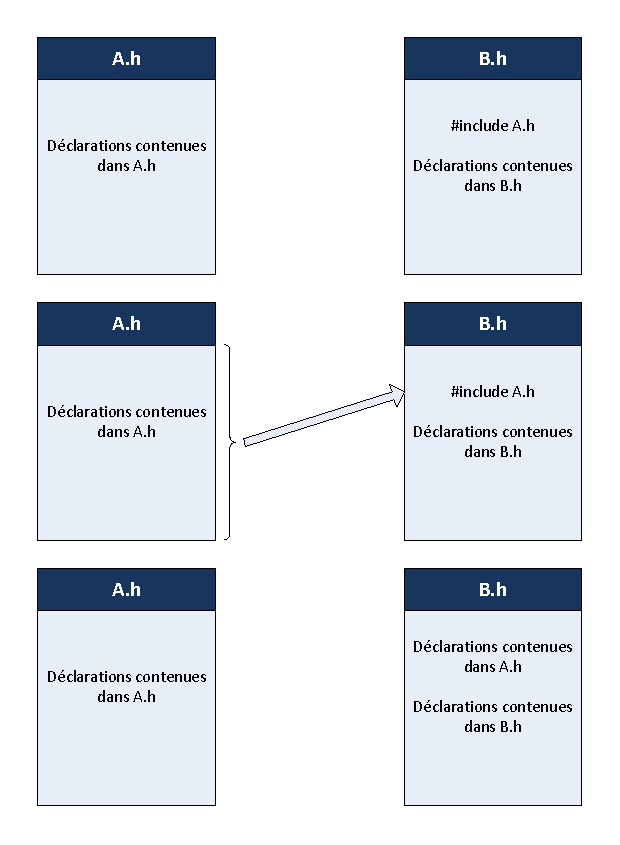
\includegraphics{../../graphes/Preprocessing.pdf}
\caption{Pendant l'�tape de pr�processing, tout se passe comme si les d�clarations contenues dans A.h �taient ajout�es en en-t�te du fichier B.h}
\label{fig:preprocessing1}
\end{figure}

L'utilisation des guillemets sp�cifie au compilateur qu'il doit trouver le fichier A.h dans le r�pertoire courant de travail (c'est � dire le r�pertoire dans votre arborescence de fichier o� se trouve votre projet). C'est en r�gle g�n�rale l'utilisation habituelle que vous en ferez. Cependant, lorsque vous utiliserez des fonctions d�finies non pas par vous mais dans le "noyau" du langage, vous utiliserez non plus des guillemets mais des $<>$ pour sp�cifier au compilateur qu'il doit aller chercher ce fichier dans les r�pertoires standards de votre IDE. Exemple :\\

\begin{DDbox}{\linewidth}
\begin{lstlisting}
#include <iostream>
\end{lstlisting}
\end{DDbox}

\subsection{Les \#define}

La commande \#define est initialement utilis�e pour faire des substitutions de cha�nes de caract�res � l'int�rieur du fichier dans lequel elle est �crite. Le pr�-processeur va donc parcourir le fichier et remplacer toutes les occurences de la variable ainsi d�finie. Ainsi, la commande :\\

\begin{DDbox}{\linewidth}
\begin{lstlisting}
#define PI 3.141592653589793
\end{lstlisting}
\end{DDbox}

aura pour effet de remplacer partout dans le fichier o� cette commande est d�finie la cha�ne de caract�res PI par la cha�ne de caract�res 3.141592653589793. Il faut vraiment comprendre cette op�ration comme de la substitution de texte.

\begin{habitudes}[Const et \#define]{Sauf raison sp�cifique, le lecteur est encourag� � pr�f�rer l'emploi de const (d�fini plus bas) plut�t que de recourir � des \#define. Comme le pr�cise Scott Meyers dans \cite{EffCpp}, l'utilisation d'un \#define devient invisible d�s la fin de l'�tape de pr�processing, ce qui peut rendre plus complexe le d�bugging dans certains cas de compilation. De plus, une variable est g�n�r�e pour chaque r�f�rence dans le code � un \#define, alors que l'utilisation d'un const ne g�n�re la cr�ation que d'une seule variable.}
\end{habitudes}

\subsection{Les \#ifndef, \#endif}

Il est possible en C++ de faire de la compilation conditionnelle. C'est � dire qu'une partie de votre code source peut � votre demande n'�tre compil�e que sous certaines conditions. La compilation conditionnelle repose sur la d�finition de variables de pr�-processing, variables qui n'existent qu'avant l'�tape de pr�-processing. Voici un exemple de telles variables :\\

\begin{DDbox}{\linewidth}
\begin{lstlisting}
#ifndef PI
#define PI 3.141592653589793
#endif
\end{lstlisting}
\end{DDbox}

Gr�ce � ces variables\footnote{qui ne doivent pas �tre utilis�es pour d'autres raisons d'ailleurs.}, nous allons pouvoir faire de la compilation conditionnelle, c'est � dire nous assurer qu'une partie de notre code ne sera compil�e que si certaines conditions sont remplies. La compilation conditionnelle est principalement utilis�e pour emp�cher le compilateur de boucler � l'infini : reprenons notre exemple du fichier header B.h qui inclut le fichier A.h (via un include). Supposons maintenant que le fichier A.h inclut lui-m�me le fichier B.h. Que se passe-t-il par d�faut ? Lorsque le pr�-processeur lit l'instruction \#include "A.h" dans le fichier B.h, il inclut le contenu de A.h dans B.h, ce faisant, il lit le contenu qu'il ins�re et le pr�-processe. Dans A.h, l'instruction \#include "B.h" est ex�cut�e, et B.h est inclus dans A.h qui est inclus dans B.h, qui est inclus dans A.h, et ainsi de suite. Au bout d'un certain temps, votre compilateur rend l'�me et votre compilation �choue.\\

\begin{figure}
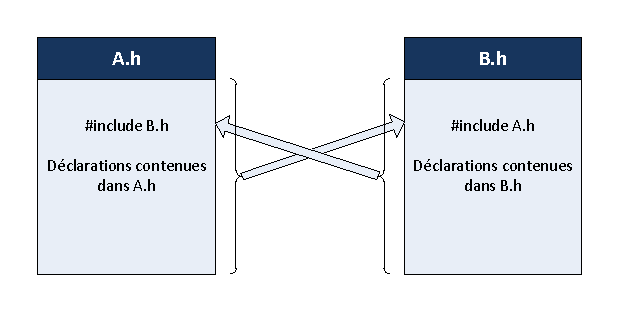
\includegraphics{../../graphes/Preprocessing2.pdf}
\caption{Exemple d'inter-d�pendance de deux fichiers headers. Si rien n'est fait pour l'�viter, le compilateur va "boucler" � l'infini en ajoutant dans chaque header le contenu de l'autre.}
\label{fig:preprocessing2}
\end{figure}

Pour �viter ceci, nous allons donc recourir � la compilation conditionnelle; dans chaque fichier, nous adoptons un m�canisme qui s'assure que le code n'est inclus/compil� qu'une seule fois, m�me en cas d'inclusion multiple.\\

Le code du fichier A.h s'organise alors de la sorte:

\begin{DDbox}{\linewidth}
\begin{lstlisting}
#ifndef A_H //Following code run only if
#define A_H //A_H is not already defined

/* Content of A.h */

#endif
\end{lstlisting}
\end{DDbox}

et le fichier B.h s'�crit de la m�me mani�re :\\

\begin{DDbox}{\linewidth}
\begin{lstlisting}
#ifndef B_H //Following code run only if
#define B_H //B_H is not already defined

/* Content of B.h */

#endif
\end{lstlisting}
\end{DDbox}

\begin{habitudes}[Compilation conditionnelle]
Tous les fichiers d'en-t�te que vous cr�ez doivent de la m�me mani�re contenir leur code entre les instructions \#ifndef et \#endif. \footnote{Il est possible de remplacer cette syntaxe par un \#pragma once, mais ceci n'est pas d�fini par la norme C++ : cette instruction est reconnue par Visual Studio mais pas par d'autres IDE, c'est pourquoi nous vous la d�conseillons et n'en parlons pas plus avant.}.
\end{habitudes}

\subsection{Les macros}
\label{sec:macros}

Les macros sont des fonctions d�finies gr�ce � une instruction \#define. Elles permettent de d�finir des fonctions qui n'existeront plus � la compilation : tout comme les variables d�finies par un \#define sont remplac�es avant la compilation par leur valeur, les fonctions d�finies par un \#define sont remplac�es par la liste de leurs instructions. Un int�r�t que nous pourrions trouver � cette technique est de supprimer l'appel � une fonction (parfois co�teux). Nous proposons � titre illustratif un exemple de macro.\\


\begin{DDbox}{\linewidth}
\begin{lstlisting}
#define MULTIPLICATE(x,y) x*y
\end{lstlisting}
\end{DDbox}

Partout o� dans notre code un appel est fait � la macro MULTIPLICATE, le pr�processeur remplace l'appel � cet macro par le produit des deux arguments, sans appeler une fonction.\\

En r�alit�, les macros sont tr�s dangereuses car particuli�rement contre-intuitives. Puisqu'il ne s'agit pas d'appel � une fonction mais bien de substitution syntaxique du pr�processeur, elles g�n�rent souvent des comportements non attendus. L'utilisation de macros avait un sens il y a 20 ans, mais il n'en a plus aucun aujourd'hui\footnote{On leur pr�f�re maintenant des fonctions templat�es inlin�es, qui ont les m�mes avantages, mais pas leurs inconv�nients.}.
A titre d'exemple seulement, nous pr�sentons trois cas simples dont les r�sultats, erron�s, doivent vous dissuader d'utiliser des macros:\\

\begin{DDbox}{\linewidth}
\begin{lstlisting}
#define MULTIPLICATE(x,y) x*y
\end{lstlisting}
\end{DDbox}

Appliquons la macro MULTIPLICATE en a+1 et b+1 :\\

\begin{DDbox}{\linewidth}
\begin{lstlisting}
double y = MULTIPLICATE(a+1,b+1);
\end{lstlisting}
\end{DDbox}

Nous obtenons en expression litt�rale :\\

\begin{DDbox}{\linewidth}
\begin{lstlisting}
y = a + 1*b + 1 = a + b + 1
\end{lstlisting}
\end{DDbox}

Ce qui est tout � fait diff�rent du r�sultat anticip�. Ceci est d� au fait que l'�tape de pr�processing est uniquement une �tape de substitution syntaxique. Dans le cas pr�sent, il manque des parenth�ses � notre macro, que nous corrigeons alors par :\\

\begin{DDbox}{\linewidth}
\begin{lstlisting}
#define MULTIPLICATE(x,y) (x)*(y)
\end{lstlisting}
\end{DDbox}

Cette fois-ci, l'utilisation de la macro dans le cas pr�c�dent donne bien le r�sultat attendu. Cependant, dans le cas de l'expression suivante, la macro donne encore un r�sultat erron� :\\

\begin{DDbox}{\linewidth}
\begin{lstlisting}
6 / MULTIPLICATE(2,3)
\end{lstlisting}
\end{DDbox}

Nous obtenons l'expression litt�rale :\\

\begin{DDbox}{\linewidth}
\begin{lstlisting}
6 / 2 * 3 = 3 * 3 = 9
\end{lstlisting}
\end{DDbox}

Essayons alors la macro SQUARE :\\

\begin{DDbox}{\linewidth}
\begin{lstlisting}
#define SQUARE(x) ((x)*(x))
\end{lstlisting}
\end{DDbox}


Nous vous laissons � titre d'exercice deviner pourquoi la variable y prend la valeur 6 dans le cas suivant :\\

\begin{DDbox}{\linewidth}
\begin{lstlisting}
int x = 1;
int y = SQUARE(x++);
\end{lstlisting}
\end{DDbox}

La conclusion de ce paragraphe est donc la suivante :\\

\begin{habitudes}[Utilisation des macros]
N'utilisez jamais de macros.
\end{habitudes}

\subsection{Templates}

C'est pendant l'�tape de pr�-processing que les classes et fonctions templat�es sont cr��es. Selon l'usage des templates que vous aurez, cette phase pourra �tre r�duite � sa plus simple expression ou au contraire se r�v�ler tr�s longue \footnote{Le lecteur int�ress� par le pr�-processeur d�couvrira avec joies les d�lices du m�ta-programming, ou de la compilation avec Boost...}. Nous reviendrons sur ce point dans le chapitre consacr� aux templates.

\section{La compilation}

A la suite du pr�-processing, vient la deuxi�me �tape de la compilation dans laquelle le compilateur compile chaque fichier source (.cpp), c'est-�-dire qu'il transforme chacun de ces fichiers sources en fichiers binaires (.o ou .obj) contenant du code directement ex�cutable par la machine. Cette phase constitue la compilation proprement dite.

\begin{habitudes}[Compilation r�guli�re]
Compilez votre code d�s que possible. Quoi qu'il arrive, compilez au moins une fois par heure. Lorsque vous d�butez, compilez toutes les 5 minutes. Si la compilation �choue, r�glez les erreurs de compilation avant de continuer � d�velopper. Si vous travaillez dans un IDE correct, il vous montrera les probl�mes de code avant m�me que vous ne compiliez; r�glez les d�s que vous les voyez.\\

Dans un environnement professionnel, vous disposerez d'int�gration continue via un serveur de build\footnote{Si ce n'est pas le cas, changez de soci�t�.}. Veillez � ne pas casser le build.
\end{habitudes}

\section{L'�dition des liens}

Enfin, le linker (ou �diteur de liens en fran�ais) agr�ge chaque fichier .o ou .obj (avec �ventuellement d'autres fichiers binaires si vous avez utilis� des librairies externes). Le linker va faire les liens entre les fichiers binaires g�n�r�s en permettant de localiser le code correspondant aux appels de fonctions. Le linker v�rifie en particulier que chaque fonction appel�e dans le programme n'est pas seulement d�clar�e (ceci est fait lors de la compilation) mais aussi bien d�finie (chose qu'il n'avait pas v�rifi�e � ce stade). Il v�rifie aussi qu'une fonction n'est pas impl�ment�e dans plusieurs fichiers .o. A la fin de l'�dition des liens, un ex�cutable est cr��.

\section{Un exemple �l�m�ntaire}

Nous disposons d'un projet contenant les fichiers main.cpp, A.cpp, B.cpp, A.h, B.h. Le fichier main.cpp fait r�f�rence au code contenu dans les fichiers A et B, le fichier A fait r�f�rence � B.\\

\begin{DDbox}{\linewidth}\begin{lstlisting}
///////////////////////////main.cpp//////////////////////
#include "A.h"
#include "B.h"

void main()
{
    functionInA();
    functionInB();
}

\end{lstlisting}
\end{DDbox}

\begin{DDbox}{\linewidth}\begin{lstlisting}
///////////////////////////A.h////////////////////////////

#ifndef A_H
#define A_H

#include "B.h" //not useful here, just put to illustrate the compilation process

void functionInA(void);

#endif
\end{lstlisting}\end{DDbox}

\begin{DDbox}{\linewidth}\begin{lstlisting}
//////////////////////////B.h//////////////////////////////
#ifndef B_H
#define B_H

void functionInB(void);

#endif

\end{lstlisting}\end{DDbox}

\begin{DDbox}{\linewidth}\begin{lstlisting}
////////////////////////////////////////////A.cpp///////////////////////////////////
#include "A.h"
#include "B.h"

void functionInA(void)
{
    functionInB();
}

\end{lstlisting}\end{DDbox}

\begin{DDbox}{\linewidth}\begin{lstlisting}
////////////////////////////////////////////B.cpp///////////////////////////////////
#include "B.h"

void functionInB(void)
{
    //Do Nothing
}

\end{lstlisting}\end{DDbox}

Le pr�processeur copie :

\begin{itemize}
\item les d�clarations de B.h dans A.h,
\item les d�clarations de A.h et B.h dans main.cpp,
\item les d�clarations de A.h et B.h dans A.cpp,
\item les d�clarations de B.h dans B.cpp
\end{itemize}

Le fait d'utiliser les \#ifndef \#endif nous permet d'�viter d'inclure deux fois les d�clarations de B.h dans main.cpp et A.cpp, ce qui am�nerait � des erreurs de compilation.\\

Une fois le preprocessing achev�, le compilateur convertit chaque fichier .cpp en un fichier binaire .o ou .obj (selon le compilateur). Lorsque les fichiers main.obj, A.obj et B.obj sont cr��s, l'�diteur des liens permet de matcher les fonctions, c'est � dire que l'�diteur des liens parcourt les fichiers .obj pour trouver la fonction functionInB() appel�e dans la fonction functionInA(). Cette fonction est trouv�e dans B.obj, et l'�diteur de lien indique que lorsque functionInA() appellera functionInB(), il faudra ex�cuter le code pr�sent dans B.obj. L'�diteur de lien fait de m�me pour les fonctions functionInA() et functionInB() utilis�es dans main.obj. Lorsque tous les appels � des m�thodes ext�rieures sont r�solus, l'�diteur de lien r�assemble tous les fichiers .obj en un fichier ex�cutable (.exe) ou en une librairie (.dll).

\section{Librairies standard}

\subsection{... du C++ standard}

De nombreuses librairies open-source sont disponibles pour le C++, mais les librairies "de base" sont assez limit�es par rapport � d'autres langages plus r�cents qui en contiennent plus. Par exemple, il n'existe pas de librairie native pour parser du XML, pour faire une requ�te HTTP, pour acc�der � une base de donn�es SQL, pour faire du threading ou �crire des Regex\footnote{Le C++11, non trait� dans ce cours, fournit maintenant certaines de ces fonctionnalit�s dans les librairies standard.}. Toutes ces librairies existent bien s�r, mais elles ne sont pas int�gr�es au langage et doivent �tre install�es et configur�es pour �tre accessibles depuis votre IDE.\\

Dans les sous-sections qui suivent, nous brossons un tableau tr�s sommaire de quelques librairies standard que vous serez probablement amen�s � utiliser, et qu'il vous sera possible d'utiliser juste en faisant mention du \#include correspondant, sans rien installer sur votre machine.\\

Pour utiliser une librairie standard simplement, en plus d'ajouter l'instruction \functionname{\#include} correspondante, il faut ajouter en dessous la ligne "using namespace std;" pour sp�cifier � l'environnement qu'il doit �galement chercher la d�claration des classes et fonctions dans "l'espace de nommage standard". Nous ne d�taillons pas plus avant la th�orie de cette n�cessit�, mais les extraits de code qui suivent �claireront par l'exemple.\\

\subsubsection{<iostream>}

La librairie \classname{<iostream>} est la biblioth�que standard pour afficher un message dans la console ou r�cup�rer un ensemble de lettres ins�r�es par un utilisateur. L'op�rateur pour afficher un message � l'�cran est l'op�rateur \functionname{cout}. Cet op�rateur s'accompagne de l'op�rateur \functionname{<<} qui indique quel est le message � afficher � l'�cran.\\

\begin{DDbox}{\linewidth}
\begin{lstlisting}
#include <iostream>
using namespace std;

void main()
{
    cout << "Hello World";
}
\end{lstlisting}
\end{DDbox}

Vous pouvez �galement afficher dans la console la valeur de variables de types primitifs. Ainsi, l'instruction suivante affiche-t-elle 2 � l'�cran : \\

\begin{DDbox}{\linewidth}
\begin{lstlisting}
#include <iostream>
using namespace std;

void main()
{
    int a = 2;
    cout << a;
}
\end{lstlisting}
\end{DDbox}

Pour aller � la ligne, vous pourrez utiliser le caract�re du retour-charriot : "$\setminus n$". Enfin, vous pouvez encha�ner plusieurs messages � afficher en les s�parant par l'op�rateur \functionname{<<}. Ainsi, les instructions suivantes affichent-elles "The value of a is 2" et le prochain message sera affich� � la ligne suivante;\\

\begin{DDbox}{\linewidth}
\begin{lstlisting}
#include <iostream>
using namespace std;

void main()
{
    int a = 2;
    cout << "The value of a is" << a << "\n";
}
\end{lstlisting}
\end{DDbox}

Dans la pratique, en dehors des tous premiers programmes que vous impl�menterez en TD, nous aurons tendance � peu nous servir des op�rateurs \functionname{cin} et \functionname{cout}.\\

\subsubsection{<vector>}

La librairie \functionname{<vector>} permet d'utiliser la classe \classname{vector} qui repr�sente les tableaux dynamiques, c'est � dire les tableaux dont la taille n'est pas connue � la compilation. La motivation et l'impl�mentation de cette classe sont esquiss�es dans le chapitre \ref{chap:memory1}. Le snippet de code suivant en donne un exemple d'utilisation.\\

\begin{DDbox}{\linewidth}
\begin{lstlisting}
#include <vector>
using namespace std;

void main()
{
    int n = 10*10;
    vector v(n);
    for (int i = 0 ; i < n ; i++)
    {
        v[i] = i*2;
    }
}
\end{lstlisting}
\end{DDbox}

\subsubsection{<string>}

La librairie \functionname{<string>} permet de manipuler des cha�nes de caract�re de mani�re plus simple que par les tableaux de caract�res du C (\classname{char[]}). En voici un exemple : \\

\begin{DDbox}{\linewidth}
\begin{lstlisting}
#include <string>
using namespace std;

void main()
{
    string myMessage = "Hello World";
}
\end{lstlisting}
\end{DDbox}

\subsubsection{<math.h>}

La librairie \functionname{<math.h>} contient de multiples fonctions "math�matiques" comme l'exponentielle, le logarithme, les fonctions min et max, les fonctions d'arrondi, les fonctions puissances et racine carr�e, les fonctions trigonom�triques, etc.

\subsubsection{<fstream>}

La librairie \functionname{<fstream>} permet d'int�agir en lecture et en �criture avec des fichiers stock�s sur le disque. Cette librairie reprend l'usange des op�rateurs de flux \functionname{<<} et \functionname{>>} de \varname{<iostream>}. L'exemple suivant cr�e un fichier "SomeExample.txt" et y �crit une ligne de texte.\\

\begin{DDbox}{\linewidth}
\begin{lstlisting}
#include <fstream>
using namespace std;

int main () {
  ofstream myfile;
  myfile.open ("SomeExample.txt");
  myfile << "Writing something to this file.\n";
  myfile.close();
  return 0;
}
\end{lstlisting}
\end{DDbox}

\subsubsection{<exception>}

La librairie \functionname{<exception>} contient un ensemble de fonctions relatives � la gestion des exceptions en C++. Parmi elles, des exceptions handlers et des m�thodes pour relancer les exceptions.\\

\subsubsection{<random>}

La librairie \functionname{<random>} fournit diff�rents g�n�rateurs de nombres al�atoires ainsi que la simulation de nombreuses loi diff�rentes.\\

\subsection{... du C++11}

Certaines biblioth�ques ont �t� ajout�es au standard dans la nouvelle version du C++, le C++11. Cependant, le C++11 apporte suffisamment de changements et de complexit� pour que nous renon�ions � le traiter dans ce cours. A titre de culture g�n�rale, nous listons ci-dessous quelques-unes des librairies standards les plus utiles qui ont �t� ajout�es en C++11.\\



\subsubsection{<memory>}

La libraire \classname{memory} contient les \classname{shared\_ptr<T>} depuis le C++11 (ils se trouvaient dans les versions ant�rieures du C++ dans la librairie Boost). L'utilisation et l'impl�mentation des \classname{shared\_ptr<T>} est discut�e dans le chapitre \ref{chap:memory1}.

\subsubsection{Les librairies de threading}

Le C++11 introduit enfin un cadre avec un mod�le m�moire\footnote{un mod�le m�moire est une d�finition du type de m�moire relative � un thread que peuvent observer les autres threads.} correct pour le C++, permettant ainsi de faire de mani�re raisonnable du multi-threading et de la programmation concurrente. Les librairies \functionname{<thread>}, \functionname{<mutex>}, \functionname{<condition\_variable>}, \functionname{<future>} participent � l'�laboration de ce cadre.\\

\subsubsection{<unordered\_map>}

Les \functionname{unordered\_map} sont des dictionnaires ressemblant au \functionname{map} d�j� existantes dans le standard, mais dont l'acc�s � un �l�ment donn� est plus rapide.\\

\subsubsection{<tuple>}

Les \classname{tuple} sont des containers g�n�riques pratiques pour contenir un nombre faible d'�l�ments de types diff�rents.\\

\section{Survivre � des messages d'erreurs incompr�hensibles}

\subsection{Erreurs � la g�n�ration du projet}

Lorsque vous voudrez compiler un projet, il y a fort � parier que la compilation �chouera en raison d'erreurs. Votre IDE va vous fournir un descriptif d'une ou de plusieurs erreurs qu'il a rencontr�es pendant la g�n�ration de votre projet. M�me si ces erreurs sont multiples, seule la premi�re des erreurs list�es peut �tre consid�r�e comme fiable, les autres erreurs �tant sujettes � caution (en effet, un IDE est sens� fonctionner si vous fournissez un code sans erreur. Si vous lui demandez de compiler un code pour lequel il n'est pas sens� fonctionner, il est possible qu'il ne puisse pas identifier pr�cis�ment tout ce qui l'emp�che de fonctionner). \\

Tout d�butant en informatique sait "coder", ce qui distingue un d�butant autonome d'un d�butant bloqu�, c'est sa capacit� � comprendre les messages sybillins d'erreurs de l'IDE. Dans un premier temps, il vous faudra comprendre si le premier message d'erreur retourn� est un message du pr�-processeur, du compilateur, ou de l'�diteur de lien. Dans le cas d'une erreur du compilateur, regardez le fichier et la ligne en cause : c'est probablement une erreur de syntaxe dans votre code, ou une utilisation d'une fonction  dont le compilateur ne trouve pas la d�claration en raison d'un \#include ad�quat manquant en d�but de fichier. Dans le cas d'une erreur de l'�diteur des liens (ces erreurs commencent par LNK dans Visual Studio, pour "linker"), l'IDE a bien trouv� la d�claration de la m�thode que vous utilisez, mais il n'a pas r�ussi � r�soudre sa d�finition, c'est � dire qu'il a ou bien trouv� plusieurs fonctions de m�me nom et de m�me prototype et qu'il ne sait laquelle choisir, ou bien qu'il n'a trouv� aucune fonction qui convenait.\\

\begin{habitudes}[Environnement de travail en anglais]
Efforcez-vous d'avoir un IDE enti�rement en anglais. Tout d'abord, puisque plus r�pandues, les versions anglophones des logiciels sont toujours moins bugg�es, ensuite parce que si vous avez un message d'erreur que vous n'arrivez pas � interpr�ter, une recherche dans google du message d'erreur en anglais vous m�ne souvent � une solution, alors que la m�me recherche sur le message d'erreur fran�ais vous apportera trop souvent : "Your search - ****** - did not match any documents."
\end{habitudes}

\subsection{Divide and Conquer}

Que vous ayez des probl�mes � la compilation ou � l'ex�cution, si les messages d'erreur que vous obtenez ne sont pas suffisament explicites et que vous n'arrivez pas � diagnostiquer votre probl�me, adoptez une d�marche dichotomique pour isoler la section de votre code fautive. Compilez/ex�cutez votre code en y enlevant certaines parties, et it�rez ainsi afin de circonscrire la partie du code en d�faut.

\subsection{Stack Overflow}

Une fois votre probl�me isol�, la r�solution devrait vous para�tre �vidente. Dans le cas contraire, apr�s vous �tre soigneusement assur�s que vous ne pouviez trouver d'explications sur internet � votre probl�me isol�, vous pouvez le poster sur Stack Overflow (http://stackoverflow.com) avec un maximum d'explications et en veillant � bien respecter les r�gles de r�daction\footnote{http://stackoverflow.com/help/how-to-ask}.\\

Toutes les questions correctement formul�es recoivent une r�ponse correctement formul�e dans l'heure.










\begin{savequote}
"I spent a few weeks... trying to sort out the terminology of "strongly typed," "statically typed," "safe," etc., and found it amazingly difficult.... The usage of these terms is so various as to render them almost useless.", Benjamin C. Pierce, in \textit{Types and Programming Languages}\\

There are 10 types of people in the world: Those who understand binary, and those who don't. \end{savequote}

\chapter{Variables et Typage}
\label{chapter:variableEttypage}

\textit{Vous �tes familiers avec les mots clefs int, short, long, double et float, et avec la base 2 ? sautez ce chapitre en premi�re lecture.}\\

\textit{Remarque pr�liminaire} : L'alphabet d'un ordinateur est limit� aux signes 0 et 1, ce qui correspond � une porte �lectronique ouverte ou ferm�e, et cet �tat est repr�sent� par un bit. Avec un ensemble de n bits, nous pouvons former $2^n$ combinaisons diff�rentes, et donc stocker au plus $2^n$ valeurs diff�rentes. Toutes les variables ont besoin de plusieurs bits pour d�finir leur valeur, et l'unit� de r�f�rence pour la taille m�moire est l'octet (byte en anglais), c'est � dire un paquet de 8 bits cons�cutifs \footnote{On prendra donc bien garde � ne pas confondre bit et byte (=8 bits). Certains providers internet abusent d'ailleurs de cette confusion en affichant les d�bits garantis en terme de Mbits/secs, c'est pourquoi vous avez une connection de 100 Mbits, mais que vous ne t�l�chargez pas � plus de quelques Mo/sec ...}. Dans ce chapitre, nous faisons un bref rappel des syst�mes de base et introduisons les diff�rents types primitifs du C++.

\section{Repr�sentation d�cimale}

La repr�sentation des nombres que nous utilisons dans la vie de tous les jours est une repr�sentation en base 10\footnote{M�me si nous utilisons �galement des vieilles bases sexag�cimales (60) d'origine babylonienne pour compter les minutes ou les secondes.}. C'est � dire qu'une dizaine est consitu�e de dix unit�s, qu'une centaine est constitu�e de dix dizaines, etc. Les bases utilis�es en informatique sont principalement des bases binaires et hexad�cimales (16), ceci �tant li� � l'alphabet r�duit � 2 caract�res (0 ou 1).

\section{Repr�sentation en base 2}

La repr�sentation en m�moire des entiers (mais aussi des d�cimaux) va utiliser le principe de l'�criture en base 2. Sur tous les processeurs PC \footnote{et depuis r�cemment sous les machines Apple, le lecteur souhaitant d�velopper sous des machines Mac un peu vieilles et utiliser des lectures disque est tr�s vivement invit� � s'enqu�rir du principe de Little et Big Endian.}, le bit le plus � gauche est utilis� comme bit de poids faible, et correspond selon sa valeur � 0 ou 1 ($2^0$). Pour le bit � sa droite, celui-ci correspond � la valeur 0 ou 2 ($2^1$), celui d'encore � droite � la valeur 0 ou 4 ($2^2$).

Quelques exemples :

\begin{align*}
10110 => 1 * 2^0 + 0 * 2^1 + 1 * 2^2 + 1 * 2^3 + 0 * 2^4 => 13\\
011 => 0 * 2^0 + 1 * 2^1 + 1 *2^2 => 6
\end{align*}

\section{les nombres n�gatifs}

Comment repr�senter un nombre n�gatif ?  Comme il n'y a que deux possibilit�s pour un nombre (positif ou n�gatif), le signe d'un nombre peut �tre repr�sent� sur un bit. Par convention, le bit de gauche d'un ensemble de bits est le bit de signe : sa valeur (0 ou 1) d�termine le signe du nombre stock� dans les bits suivants. Cel� diminue donc d'une unit� le nombre de bits disponibles pour stocker le nombre lui-m�me. Lorsque l'on travaille uniquement avec des nombres positifs, il est possible de signifier � la machine que nous voulons faire l'�conomie du bit de signe pour pouvoir travailler sur des valeurs potentiellement plus grandes. Nous revenons sur ce point au paragraphe suivant.

\section{les entiers}

Il existe en C++ 6 types d'entiers diff�rents, qui se r�partissent en deux cat�gories, les entiers sign�s et les entiers non-sign�s. Les entiers non sign�s, qui ont renonc� au bit de signe, peuvent donc prendre deux fois plus de valeurs que leurs analogues sign�s.\\

\begin{itemize}
\item Les \keyword{short} stockent un entier sur 2 octets, ils prennent des valeurs entre -32768 et +32767
\item Les \keyword{long} stockent un entier sur 4 octets, ils prennent des valeurs entre -2147843648 et +2147843647
\item Les \keyword{int} n'ont pas une taille d�finie par la spec du langage. Ils ont sur la plupart des compilateurs/machines une taille de 4 octets, et ont donc le m�me comportement que les long, mais ce n'est pas syst�matique.
\item Les \keyword{ushort} ou \keyword{unsigned short} stockent un entier sur 2 octets, ils prennent des valeurs entre 0 et +$2^{16} - 1$
\item Les \keyword{ulong} ou \keyword{unsigned long} stockent un entier sur 4 octets, ils prennent des valeurs entre 0 et +$2^{32} - 1$
\item Les \keyword{uint} ou \keyword{unsigned int} l� encore, cel� d�pend des compilateurs, mais en r�gle g�n�rale, m�me cas que les unsigned long\\
\end{itemize}

Voici deux exemples de d�clarations d'entiers.\\

\begin{DDbox}{\linewidth}\begin{lstlisting}
unsigned int currentIndex;
int matchingCount;
\end{lstlisting}\end{DDbox}

Comme nous l'avons expliqu�, signer ou non un entier a des cons\'equences sur
l'intervalle des valeurs qu'il peut prendre; ces intervalles sont
pr\'ecis\'es dans le tableau \ref{tab:bornessignes}\footnote{Les bornes pour les \keyword{int} ne sont valables que pour les architectures 32 bits.}.\\

\begin{table}
	\centering
	\begin{tabular}{c| c| c }
		Type & Minimum & Maximum \\
		\hline
		\keyword{unsigned int} & 0 & $2^{32}-1$ \\
		\keyword{int} & $-2^{31}$  & $2^{31}-1$ \\
		\hline
		\keyword{unsigned short} & 0 & $2^{16}-1$ \\
		\keyword{short} & $-2^{15}$  & $2^{15}-1$ \\
        \hline
		\keyword{unsigned long} & 0 & $2^{32}-1$ \\
		\keyword{long} & $-2^{31}$  & $2^{31}-1$ \\
		\hline
		\keyword{unsigned char} & 0 & $255$ \\
		\keyword{char} & $-128$  & $127$ \\
	\end{tabular}
	\caption{Bornes des diff\'erents types}
	\label{tab:bornessignes}
\end{table}

Que se passe-t-il lorsque l'on ajoute un � une variable enti�re qui contient la valeur maximale?
Un tel ph�nom�ne est appel� Integer Overflow. Dans le cas d'entiers sign�s, le r�sultat est impr�visible. Dans le cas d'entiers non sign�s, le r�sultat est r�duit modulo une puissance de 2. Les effets sont parfois amusants \footnote{cela donne par exemple des jolis Kill-Screen http://en.wikipedia.org/wiki/Pac-Man\#Split-screen}, c'est aussi parfois l'occasion de faire des bandes dessin�es \footnote{http://xkcd.com/571/}, mais les overflows peuvent amener des bugs tr�s p�nibles � isoler, et qui peuvent se r�v�ler catastrophique (une Ariane 5 s'est �cras�e � cause d'un overflow principalement \footnote{http://www.astrosurf.com/luxorion/astronautique-accident-ariane-v501.htm}).

\begin{habitudes}[Typage des entiers]
Nous invitons le lecteur � prendre l'habitude de ne travailler uniquement qu'avec des int, mais c'est un parti pris qui ne fait pas l'unanimit�. Ceci peut se r�v�ler probl�matique dans certains cas, notamment puisque la taille des int est laiss�e � la discr�tion du compilateur et qu'un m�me programme compil� sur une m�me machine mais avec deux compilateurs diff�rents pourra avoir des comportements diff�rents. Cependant, l'utilisation des int est en r�gle g�n�rale tr�s suffisante. La vraie raison qui nous porte � faire cette proposition est la simplicit� de votre code. Utiliser des short ou des long, c'est attirer l'attention de votre relecteur sur le fait que vous vous �tes pass�s des int, et c'est implicitement sugg�rer que ce changement est n�cessaire � l'endroit o� vous l'avez fait. Un bon code se doit d'�tre simple et banal aux points les plus simples, et n'attirer l'attention du lecteur que lorsque ceci est n�cessaire.
\end{habitudes}

\section{Les r�els}

Les nombres r�els sont stock�s autrement que les nombres entiers. Ils sont dits � virgule flottante. Les nombres � virgule flottante sont des nombres dans lesquels la position de la virgule en tant que s�parateur entre partie enti�re et partie d�cimale n'est pas fig�e. La grandeur d'un tel nombre est donn�e par un exposant de 10 ad�quat. Par exemple, le nombre 27,6 peut �tre �crit sous les 3 formes :

\begin{align*}
2,76 * 10^1\\
0,276 * 10^2\\
276 * 10 ^{-1}
\end{align*}

Dans la m�moire de la machine, un nombre r�el est d�compos� en un signe (+ ou -), en un exposant (ex : $10^1$), et une mantisse (ex : 2,76).
Comme nous avons plusieurs types pour distinguer les entiers selon les plages de valeurs que nous anticipons, nous avons �galement plusieurs types diff�rents pour stocker un r�el.\\

\begin{itemize}
\item Les \keyword{float} : sur 4 octets, mantisse sur 23 bits, exposant sur 8 bits, signe sur 1 bit. Le float garantit une pr�cision d'au moins 6 chiffres apr�s la virgule.
\item Les \keyword{double} : sur 8 octets, mantisse sur 52 bits, exposant sur 11 bits, signe sur 1 bit. Le double garantit une pr�cision d'au moins 15 chiffres apr�s la virgule.
\item Les \keyword{long double} : sur 10 octets, mantisse sur 64 bits, exposant sur 15 bits. Le long double garantit une pr�cision d'au moins 17 chiffres apr�s la virgule.
\end{itemize}

\begin{habitudes}[Typage des r�els]
Pareillement, nous vous conseillons d'utiliser uniquement des double. L'utilisation de float sugg�re � votre lecteur que vous �tes en train de faire des �conomies sur la m�moire pour faire des optimisations fines. En r�gle g�n�rale, �tant donn�s la taille des RAMs actuelles et le salaire horaire des bons d�veloppeurs, il vaut mieux avoir un programme un peu moins optimis� en emprunte m�moire (\textit{Memory footprint}) et �viter des bugs atroces qui peuvent co�ter des semaines � d�tecter et fixer\footnote{Repensez � la fus�e Ariane !}.
\end{habitudes}

\section{D�claration des variables}

Il est crucial de comprendre la diff�rence entre d�finition et d�claration. Nous renvoyons le lecteur au chapitre sur la compilation/interpr�tation si ce pas n'est pas encore clair\footnote{Nous vous avions bien dit qu'il fallait lire ce chapitre jusqu'� l'avoir compris !}.\\

Lorsque nous souhaitons d\'eclarer une variable, nous le faisons de la mani\`ere suivante :\\

\begin{DDbox}{\linewidth}\begin{lstlisting}
TypeDeLaVariable NomDeLaVariable;
\end{lstlisting}\end{DDbox}

La d\'eclaration peut \^etre effectu\'ee n'importe o\`u dans le code. Cependant, l'endroit o� elle est d�clar�e est extr�mement important, puisqu'il d�finit le scope de la variable, c'est � dire sa port�e, et pourra parfois emp�cher la compilation. Nous reviendrons sur ce point lorsque nous aurons introduit les fonctions.\\

\begin{habitudes}[D\'eclaration des variables]
	Une bonne habitude est de d\'eclarer les variables le plus tard possible dans le code, c'est � dire de minimiser leur scope, afin d'am\'eliorer la lisibilit\'e et d'aider le compilateur dans ses optimisations\footnote{Il y a des contre-exemples bien s�r, mais cel� d�passe le cadre de ce cours}.
\end{habitudes}

\begin{habitudes}[Nom des variables]
Toutes vos variables, comme tous vos fichiers, vos m�thodes et vos commentaires doivent �tre nomm�s en anglais.
\begin{enumerate}
\item L'anglais est souvent plus compact. Pouvoir exprimer une id�e en moins de lettre est extr�mement appr�ciable puisque nous voulons limiter la taille des noms des variables.
\item Certains concepts n'ont pas de traduction ad�quate et r�pandue dans notre langue.
\item Vous serez tr�s probablement amen�s � travailler en �quipe, r�guli�rement avec des gens non-francophones. Imaginez-vous devoir lire du code �crit et comment� en russe...\\
\end{enumerate}
\end{habitudes}

\begin{habitudes}[Nom des variables (2)]
Trouvez des noms courts, expressifs, sp�cifiques et non-provoquants (On est jamais � l'abri d'un bug qui soul�ve un retour windows en expliquant que l'instance z de la classe fuckstring n'a pas �t� instanci�e, devant un client/n+1/examinateur...). Une exception : pour coder une fonction math�matique, ces conseils sont diff�rents, pr�f�rez des noms de variables tr�s courts � des noms expressifs, du type x, y, z, dx, etc.
\end{habitudes}

Le listing suivant pr�sente quelques exemples de d�claration de variables.\\

\begin{DDbox}{\linewidth}\begin{lstlisting}
double threshold;
long   y;
int    length;
short  minValue;
float  mean;
char   firstLetter;
bool   isLocked;
\end{lstlisting}\end{DDbox}

\begin{table}
    \begin{tabular}{l l l l l}
    Type & Description &  Java & VBA \\
    \hline
    int  & Entier &   Integer & Integer \\
    double & Decimal double pr\'ecision  & Double & Double \\
    char & caract\`ere  & Char & char
    \end{tabular}
    \caption{Types de variables}
    \label{table:variableTypes}
\end{table}


\warning Il est important de noter que les noms des variables sont sensibles � la casse (case sensitive)\footnote{C'est-\`a-dire \`a la distinction entre majuscules et minuscules.}. En d'autres termes, cela signifie que \varname{Variable1} et \varname{variable1} d\'esignent deux variables diff\'erentes. \textbf{Nous attirons votre attention sur cette propri�t�, qui sera source dans vos premiers programmes des trois quarts des erreurs de compilation que vous rencontrerez.}

\begin{habitudes}[Usage des majuscules]

Par convention,
\begin{itemize}
\item les variables commencent par une minuscule.
\item les fonctions commencent par une majuscule.
\item les classes commencent par une majuscule.
\item les constantes commencent par une majuscule.
\item les constantes d�finies par un \#define sont enti�rement en majuscules.
\item lorsqu'un nom est la concat�nation de plusieurs mots, la premi�re lettre de chaque mot en dehors du premier prend une majuscule (ex: PerfectRedWidget).
\end{itemize}

Ces r�gles permettent de distinguer d'un seul coup d'oeil variables, classes et m�thodes et sont indispensables\footnote{Nous nous acharnerons sur vous en TD si vous ne les respectez pas.}. Elles permettent aussi de pouvoir recourir au type de syntaxe suivant, dans lequel le premier mot d�signe le type et le deuxi�me mot d�signe le nom de l'instance :\\

\begin{DDbox}{\linewidth}\begin{lstlisting}
Widget widget;
\end{lstlisting}\end{DDbox}

\end{habitudes}

\section{Les bool�ens}

Les variables de type \keyword{bool�en} contiennent un bool�en, c'est � dire une des deux valeurs suivantes : \textit{true} ou \textit{false}. Par convention, la valeur false correspond � 0, la valeur true correspond � 1. Un bool�en pourrait donc �tre stock� sur un unique bit. Cependant, puisque tous les autres types ont besoin de plusieurs octets, il aurait �t� malavis� de n'utiliser qu'un bit pour les bool�ens, puisque ceci aurait introduit des d�calages. Les bool�ens sont donc stock�s sur un octet entier.

\section{Les caract�res}

Il y a malheureusement plusieurs standards diff�rents dans l'encodage des caract�res\footnote{c.f. par exemple http://www.joelonsoftware.com/articles/Unicode.html}, tout comme il y a plusieurs types de clavier et plusieurs alphabets. C'est pourquoi vous r�cup�rez parfois des mails avec des caract�res �tranges quand vous �tes sur des OS diff�rents par exemple. Sur un octet, nous pouvons stocker 256 caract�res diff�rents. Un des standards les plus utilis�s est le standard am�ricain, ASCII. La variable caract�re est d�sign�e par le mot clef char, mais sauf cas de force majeur, utilisez plut�t des chaines de caract�res repr�sent�es (string) que des tableaux de char.

\section{Types d�finis par l'utilisateur}

La d�claration/d�finition/instanciation de variables d'un type non primitif (c'est � dire d�fini par vous-m�me) s'effectue de la m�me mani�re.
Par exemple :\\

\begin{DDbox}{\linewidth}\begin{lstlisting}
Identifier identifier = myInstance.GetId();
\end{lstlisting}\end{DDbox}

Pour la d�finition de telles variables, nous approfondirons la question dans le chapitre d�di� aux classes.\\

\section{Constantes et \'enum\'erations}
\subsection{Constantes}

R\'eguli\`erement lorsque nous \'ecrivons un programme, nous avons besoin de d\'efinir
des constantes, comme dans le listing \ref{lst:besoinconstante.cpp}.\\

\includecodecaption{besoinconstante.cpp}{N\'ecessit\'e d'une constante}

Dans le code pr�c�dent, rien n'interdit de
red\'efinir la valeur de cette ``constante'' au cours du programme. Il est
possible de rem\'edier \`a ce probl\`eme au moyen du mot cl\'e \keyword{const}, qui indique qu'une variable est constante, et ne peut \^etre modifi\'ee.\\

\begin{DDbox}{\linewidth}\begin{lstlisting}
	const type instanceName = value;
\end{lstlisting}\end{DDbox}

Le listing \ref{lst:besoinconstante.cpp} devient alors :\\

\includecodecaption{besoinconstanteresolu.cpp}{N\'ecessit\'e d'une constante}

\subsection{Enum\'erations}

Nous pouvons \'egalement avoir besoin d'une liste de constantes mais li\'ees entre elles. Consid\'erons le code du listing \ref{lst:besoinenum.cpp}.\\

\includecodecaption{besoinenum.cpp}{Une s\'erie de constantes}

Ce code pr\'esente plusieurs probl\`emes :

\begin{itemize}
		
	\item Il est possible de passer une taille en dehors des valeurs de la liste de constantes. Par ailleurs, rien ne garantit que c'est bien une taille que nous allons passer;
	\item Si nous voulons rajouter de nouvelles tailles, il faut g\'erer soi-m\^eme l'attribution de nouvelles valeurs (4, 5, 6, etc.).\\
		
\end{itemize}

Le langage C++ fournit une m\'ethode automatique pour r\'esoudre ce probl\`eme, appell�e \'enum\'eration. Nous d\'eclarons une \'enum\'eration de la mani\`ere suivante :\\

\begin{DDbox}{\linewidth}\begin{lstlisting}
	enum NomEnumeration
	{
		premierElement,
		deuxiemeElement,
		troisiemeElement
		...
	};
\end{lstlisting}\end{DDbox}

La num\'erotation\footnote{Ce n'est d'ailleurs pas forc\'ement 1, 2, 3, etc.} est automatique. En l'occurrence, notre enum\'eration s'\'ecrirait :\\

\begin{DDbox}{\linewidth}\begin{lstlisting}
	enum Size
	{
		Small,
		Medium,
		Big
	}
\end{lstlisting}\end{DDbox}

Le listing \ref{lst:besoinenum.cpp} devient alors :\\

\includecodecaption{besoinenumresolu.cpp}{Emploi d'une \'enum\'eration}

L'emploi d'une \'enum\'eration a donc r\'esolu nos probl\`emes :\\

\begin{itemize}

	\item Un m�canisme garantit que c'est bien une valeur valable qui sera pass�e en argument de la fonction f.
	\item Nous pouvons rajouter de nouvelles valeurs sans nous pr\'eoccuper de la
		num\'erotation.
	\item Le code obtenu est nettement plus lisible.
		
\end{itemize}

\section{Tableaux statiques}

Il est possible en C++ de d\'eclarer un \index{tableau}tableau de variables. Cela se fait de
la mani\`ere suivante :\\

\begin{DDbox}{\linewidth}
\begin{lstlisting}[caption=D\'eclaration d'un tableau]
Type arrayName[size];
\end{lstlisting}
\end{DDbox}

Par exemple,\\

\begin{DDbox}{\linewidth}
\begin{lstlisting}
double someArray[ 50 ];
\end{lstlisting}
\end{DDbox}

permet de d\'eclarer un tableau de 50 nombres r�els en double pr\'ecision.\\

Nous acc\`edons alors aux \'el\'ements du tableau \`a l'aide de l'op\'erateur \texttt{[ ]}. Pour cr\'eer un tableau
de 10 \'el\'ements et y ranger les carr\'es des entiers de 1 \`a 10, nous \'ecririons:\\

\begin{DDbox}{\linewidth}
\begin{lstlisting}[caption=Utilisation d'un tableau]
double someArray[ 10 ];

for( int i = 0 ; i < 10 ; i++)
{
    someArray[i]=(i+1)*(i+1); //All arrays start at index 0
}
\end{lstlisting}
\end{DDbox}

La syntaxe \'equivalente en Python ou en VBA serait :
\begin{center}%
    \begin{minipage}{0.45\linewidth}
       \begin{center}\emph{Python}\end{center}
\begin{DDbox}{\linewidth}
\begin{lstlisting}[language=python]
#c'est une liste et
#non un tableau
tableau = []

for i in range(1, 11):
	tableau.append(i * i)
\end{lstlisting}
\end{DDbox}
    \end{minipage}
    \qquad
    \begin{minipage}{0.45\linewidth}%
    \begin{center}\emph{VBA}\end{center}
\begin{DDbox}{\linewidth}
\begin{lstlisting}[language=VBScript]
dim i as Integer
dim tableau(10) as Integer

for i=1 to 10
    tableau(i)=i*i
next i
\end{lstlisting}
\end{DDbox}
    \end{minipage}
\end{center}

Pour cr�er un tableau dont la taille n'est pas une constante �crite nomm�ment dans le code, c'est beaucoup plus difficile; nous reviendrons sur ce point dans le chapitre \ref{chapter:memory}.\\

\section{Op�rations de conversion / casting}

L'op�ration de convertir une variable d'un certain type en une variable d'un autre type s'appelle conversion de type, ou \textit{type casting}. Nous utiliserons indiff�remment les deux d�nominations.\\

\subsection{Conversions implicites}

Les conversions implicites, comme leur nom l'indique, ne requiert aucune op�ration de votre part et sont r�alis�es automatiquement par l'environnement. Ainsi le code suivant est correct : \\

\begin{DDbox}{\linewidth}
\begin{lstlisting}[language=C++,label="conversionImplicite", caption="Conversion implicite"]
float pi = 3.14;
double pii = pi;
\end{lstlisting}
\end{DDbox}

Il existe de nombreuses conversions implicites pour les types primitifs, comme les conversions suivantes : short => int, int => float, float=>double, double => int, etc.\\

\warning Il existe aussi des conversions implicites qui sont beaucoup moins �videntes. Ainsi, si le type \classname{B} poss�de un constructeur qui prenne en argument une instance de type \classname{A}, le cast implicite suivant est l�gal :\\

\begin{DDbox}{\linewidth}
\begin{lstlisting}[language=C++,label="conversionImplicite2", caption="Conversion implicite par le constructeur"]
class A {};
class B { public: B (A a) {} };

A a;
B b=a;
\end{lstlisting}
\end{DDbox}

C'est clairement une fonctionnalit� WhatTheFuck du langage, mais elle reste assez agr�able pour la d�claration de SmartPointer, cf chapitre \ref{chap:memory1}.\\

\subsection{Conversions explicites}

Pour de nombreuses autres conversions, il est n�c�ssaire d'expliciter l'op�ration de conversion. Cette explicitation se r�alise en mettant � gauche de la variable que l'on souhaite convertir (caster) le type vers lequel nous souhaitons convertir, encadr� par des parenth�ses. Ainsi, la conversion suivante est-elle r�alis�e explicitement : \\

\begin{DDbox}{\linewidth}
\begin{lstlisting}[language=C++,label="conversionExplicite", caption="Conversion explicite d'un short en int"]
short s = 200;
int b = (int) s;
\end{lstlisting}
\end{DDbox}

Deux fonctions ou deux op�rateurs peuvent avoir le m�me nom, mais poss�der des arguments de type diff�rents, et avoir ou non le m�me comportement. Ainsi, l'op�rateur "/" (lire "divis� par") est-il d�fini diff�remment pour des entiers et pour des r�els. Dans le cas o� \varname{a} et \varname{b} sont des entiers, le r�sultat de \varname{a/b} est le quotient dans la division euclidienne de \varname{a} par \varname{b}. Ainsi, si \varname{a} vaut 16 et \varname{b} vaut 17, le r�sultat de \varname{a/b} vaut 0. Cependant, si \varname{c} et \varname{d} sont deux r�els, alors le sens de \varname{c/d} correspond au quotient r�el, qui vaut une valeur proche de 1, m�me si \varname{c} et \varname{d} ont pour valeur un entier.\\

\begin{DDbox}{\linewidth}
\begin{lstlisting}[language=C++,label="division", caption="Divisions r�elles et euclidiennes"]
int a = 16;
int b = 17;
int q1 = a/b; //q1 = 0

double c = 16;
double d = 17;
double q2 = c/d // q2 = 0.94117647058
\end{lstlisting}
\end{DDbox}

Ainsi, lorsque nous voudrons estimer un quotient de deux entiers, il faudra bien prendre garde que sauf mention du contraire, le quotient calcul� sera celui de la division euclidienne. Si nous voulons obtenir le quotient r�el, il nous faut caster au moins un des deux arguments en r�el, comme dans le listing suivant, afin de faire comprendre au compilateur que nous ne voulons pas du quotient euclidien.\\

\begin{DDbox}{\linewidth}
\begin{lstlisting}[language=C++,label="division2", caption="Cast d'un entier en double pour obtenir une division r�elle"]
int a = 16;
int b = 17;
double q1 =((double) a)/b; //q = 0.94117647058
\end{lstlisting}
\end{DDbox}

\subsection{Ind�cisions sur les cast}

De mani�re semblable, d�finissons une fonction Power, qui prenne en argument deux r�els \varname{x} et \varname{y} pour calculer $x^y$.\\

\begin{DDbox}{\linewidth}
\begin{lstlisting}[language=C++,label="power1", caption="Une premi�re fonction Power"]
#include <math.h>
double Power(double x, double y)
{
    return exp(y*log(x));
}
\end{lstlisting}
\end{DDbox}

Nous pouvons donner en argument � cette fonction un entier, l'environnement se chargeant de r�aliser le cast implicitement.\\

\begin{DDbox}{\linewidth}
\begin{lstlisting}[language=C++,label="power1bis", caption="Un autre cast implicite"]

void main()
{
    int a = 3;
    int b = 2;
    double c = Power(a,b);
}

\end{lstlisting}
\end{DDbox}

D�finissons ensuite la m�me fonction Power dont les arguments sont cette fois-ci des \classname{float}.\\

\begin{DDbox}{\linewidth}
\begin{lstlisting}[language=C++,label="power2", caption="Une deuxi�me fonction Power"]
#include <math.h>
float Power(float x, float y)
{
    return exp(y*log(x));
}
\end{lstlisting}
\end{DDbox}

Nous ne pouvons plus maintenant r�aliser de conversion implicite, car l'environnement ne sait s'il doit caster nos entiers en \classname{double} et utiliser la premi�re fonction, ou bien caster nos entiers en \classname{float} et utiliser la deuxi�me fonction. Ainsi � la compilation, nous obtenons un message d'erreur semblable au suivant : \\

\begin{DDbox}{\linewidth}
more than one instance of overloaded function "Power" matches the argument list:
    function "Power(double x, double y)"
    function "Power(float x, float y)"
argument types are: (int, int)
\end{DDbox}

Il nous faut donc ici r�aliser un cast explicite pour lever l'ambigu�t�.\\

\begin{DDbox}{\linewidth}
\begin{lstlisting}[language=C++,label="power2bis", caption="Le cast explicite est ici indispensable"]

void main()
{
    int a = 3;
    int b = 2;
    double c = Power( (double) a, (double) b);
}

\end{lstlisting}
\end{DDbox}

Bien que le C++ soit statiquement typ� (cf paragraphe suivant) et que cel� garantisse que de nombreuses erreurs de typage aient lieu � la compilation plut�t qu'� l'ex�cution (ce qui r�duit tr�s fortement leur potentiel de nuisance), il est possible de tromper le compilateur via toutes sortes d'horreurs r�sultant de casts explicites, et ainsi de passer les v�rifications � la compilation et d'�chouer seulement � l'ex�cution. Pour se pr�munir au moins partiellement de ces probl�mes, il existe diff�rents op�rateurs de cast suppl�mentaires (\functionname{dynamic\_cast<T>, static\_cast<T>, reinterpret\_cast<T>} et \functionname{const\_cast<T>}), mais ceci d�passe le cadre de notre cours.\\

\section{Le typage du C++}

Le C++ est un langage typ\'e de mani\`ere statique. Cela signifie que les variables doivent \^etre d\'eclar\'ees et leur types explicit\'es, � la diff�rence par exemple du python o� une m�me variable peut contenir successivement un entier puis une cha�ne de caract�re ou un double. Le compromis qui se cache derri�re ce choix est un compromis souplesse / performance et garantie. Devoir d�terminer � l'ex�cution le type d'une variable plut�t que de l'avoir d�termin� statiquement a un certain co�t. Les types n'existent en C++ qu'� la compilation, c'est � dire qu'� l'execution il n'est plus possible de r�cup�rer le type d'un objet; cette limitation ne se retrouve pas dans des langages plus r�cents comme le C\#.\footnote{En C\#, on peut par exemple r�cup�rer le type d'un objet � l'ex�cution, parcourir l'ensemble des types charg�s en m�moire, s�lectionner les types qui h�ritent de telle classe et qui poss�dent un constructeur vide, les instancier, etc.}.


\begin{savequote}
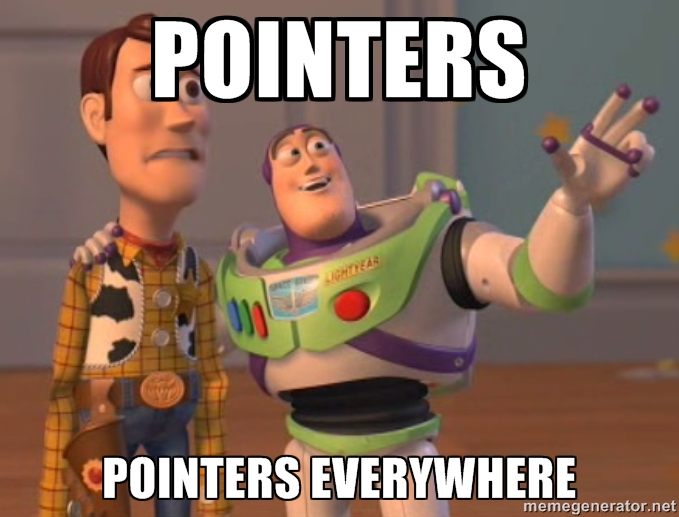
\includegraphics[scale=0.4]{../../Pictures/PointersEverywhere.jpg}
\end{savequote}

\chapter{Les pointeurs}


\section{D�finition des pointeurs}

Comme nous l'avons expliqu� pr�c�demment, le C++ permet � la fois de manipuler des abstractions puissantes mais aussi d'�tre tr�s proche de la machine quand cel� est n�cessaire. Dans ce chapitre, nous nous pla�ons � un niveau d'abstraction tr�s bas pour pr�senter les pointeurs.\\

Chaque variable d'un programme est stock�e dans une des m�moires de la machine qui ex�cute le code (m�moire Cache, m�moire RAM, disque dur, etc.). Nous pouvons pour le moment consid�rer la m�moire de notre machine comme un ensemble de cases m�moires contig�es, chacune d'un octet. Chaque case est num�rot�e, afin de pouvoir rapidement acc�der � une case pr�cise. Lorsque nous �crivons :\\

\begin{DDbox}{\linewidth}\begin{lstlisting}
unsigned int n=3;
\end{lstlisting}\end{DDbox}

nous pouvons acc�der de deux mani�res diff�rentes � la valeur de notre variable : la premi�re en faisant appel au nom de la variable, c'est � dire en invoquant son nom -n-, la deuxi�me en allant chercher directement en m�moire � l'adresse de notre variable la valeur qui s'y trouve. Dans le cas qui nous int�resse ici, la variable n a �t� stock�e sur 4 octets, par exemple de cette mani�re :

\begin{center}
\begin{tabular}{l|l|l|l|l|l|l|l|l|l|l}
Case m\'emoire & 0 & 1 & 2 & 3 & 4 & 5 & 6 & 7 & 8 & 9 \\
\hline
Nom &  &  &  & n  & n & n & n & &  & \\
\hline
Valeur &  &  &  & 110..000 & 00...  & 000...  & 000..  &  &  &   \\
\end{tabular}
\end{center}

Le C++ permet d'obtenir � l'ex�cution l'adresse d'une variable (qui va �videmment varier � chaque ex�cution puisque nous n'avons pas le contr�le sur l'endroit o� nos variables sont stock�es), gr�ce � l'op�rateur \&. Il nous suffit donc d'�crire \&n pour obtenir l'adresse de n. Cette adresse correspond en fait � l'index de la premi�re case m�moire dans laquelle est stock�e notre variable (Dans notre exemple ce serait la case num�ro 3). Naturellement, on pourrait penser que le type d'une adresse est donc un entier. En fait, il n'en est rien pour deux raisons :\\

\begin{itemize}
\item Il serait tr�s facile de confondre un entier et son adresse si tous les deux �taient du m�me type.
\item Pour retrouver une variable en m�moire, il ne suffit pas de conna�tre l'adresse de la premi�re case m�moire qui lui est allou�e, il faut �galement conna�tre son type. En effet, si la variable stock�e est un int ou un double, elle ne sera pas encod�e de la m�me mani�re et ne prendra pas le m�me nombre de cases m�moires. \\
\end{itemize}

Pour avoir une correspondance parfaite entre une variable et son �quivalent en m�moire, il nous faut donc conna�tre � la fois le type de la variable, et l'index de la premi�re case m�moire o� cette variable est contenue. Partant de cette remarque, nous pouvons construire un nouveau type de variable, appel� pointeur, qui va contenir les informations n�cessaires pour retrouver en m�moire la valeur de notre variable n. Nous d�clarons et d�finissons notre pointeur sur n par l'instruction suivante :\\

\begin{DDbox}{\linewidth}\begin{lstlisting}
int* pn= &n;
\end{lstlisting}\end{DDbox}

Dans l'instruction pr�c�dente, nous d�clarons une variable pn de type pointeur sur entier (int*), et nous la d�finissons en lui affectant l'adresse de n, adresse r�cup�r�e par l'op�rateur \&. Le symbole * est ici utilis� pour indiquer que pn n'est pas un entier mais un pointeur sur entier. Pour chaque type T "de base", nous avons donc un type correspondant qui est le type T*, et des variables de type T* que nous appelons pointeurs sur une instance de type T, ou, par abus de langage, simplement pointeur sur T.

\begin{habitudes}[Nom des pointeurs]
Prenez pour habitude de pr�fixer vos pointeurs par la lettre p, cel� simplifie beaucoup la relecture du code.
\end{habitudes}

Nous pourrions de la m�me mani�re d�finir un pointeur sur double :\\

\begin{DDbox}{\linewidth}\begin{lstlisting}
double b = 3.2;
double* pb = &b;
\end{lstlisting}\end{DDbox}

\section{D�r�f�renciation}

Lorsque nous disposons d'un pointeur, nous pouvons souhaiter r�cup�rer la valeur point�e, c'est � dire le \textit{d�r�f�rencer}. Pour cel�, nous utilisons l'op�rateur * --dit op�rateur de d�r�f�rencement-- pour acc�der � la valeur stock�e � l'adresse du pointeur :\\

\begin{DDbox}{\linewidth}\begin{lstlisting}
double b = 3.2;
double* pb = &b;
double c = *pb;
\end{lstlisting}\end{DDbox}

\bigskip
\begin{warning}
Nous venons de voir deux utilisations distinctes du symbole * :
\begin{enumerate}
\item lors de la d�claration d'un pointeur, il sp�cifie que la variable pb par exemple est un pointeur sur double.
\item lors de la d�r�f�renciation, c'est l'op�rateur * qui associe � un pointeur la variable vers laquelle le pointeur renvoie.
\end{enumerate}
Il s'agit donc d'une homonymie de l'op�rateur *, � laquelle il faut prendre garde lorsque l'on d�bute.
\end{warning}

\section{Op�rateurs \& et *}

Les valeurs de a et de b sont �gales � la suite des instructions suivantes :\\

\begin{DDbox}{\linewidth}\begin{lstlisting}
double a = 3.2;
double b = *(&a);
\end{lstlisting}\end{DDbox}

Les valeurs de pa et pb sont �gales � la suite des instructions suivantes :\\

\begin{DDbox}{\linewidth}\begin{lstlisting}
double a = 3.2;
double* pa = &a;
double* pb = &(*pa);
\end{lstlisting}\end{DDbox}

Les instructions suivantes sont fausses car les types ne correspondent pas, et le compilateur retournera une erreur :\\

\begin{DDbox}{\linewidth}\begin{lstlisting}
int a = 3;
double* pa = &a;
\end{lstlisting}\end{DDbox}

\subsection{Formalisation des pointeurs}

Notons E l'ensemble des variables stock�es en m�moire d'un programme fini, et P l'ensemble des pointeurs qui pourraient �tre cr��s et qui pointeraient sur une de ces variables. On peut d�finir sur P une relation d'�quivalence $\thicksim$ (r�flexive, sym�trique et transitive) par $px \thicksim py$ si et seulement si *px = *py. L'espace quotient de P par $\thicksim$ est en bijection avec E, et les op�rateurs induits $\overline{*}$ et $\overline{\&}$ induits sont alors des bijections entre E et $\overline{P}$, inverses � gauche et � droite l'un de l'autre.

\section{Usage des pointeurs}

Les pointeurs sont omnipr�sents en C++. Des librairies comme la STL tendent cependant � diminuer leur utilisation directe par l'utilisateur, et aujourd'hui, il serait presque possible d'�crire en C++ sans utiliser de pointeurs. En effet, il est possible dans la plupart des cas d'�crire du code "plus haut niveau" o� l'usage des pointeurs est cach�. N�anmoins, il est fondamental que vous compreniez bien les m�caniques sous-jacentes. Les pointeurs restent souvent indispensables (de mani�re implicite ou explicite) pour le polymorphisme, lorsque nous manipulons des instances volumineuses, dans le cas de gestion dynamique de m�moire, dans la construction de la plupart des Design Pattern, ...\\

Les chapitres suivants montreront de nombreux exemples d'utilisation de pointeurs.


\begin{savequote}
"Dis-moi comment tu traites les fonctions, je te dirai quel type de langage tu es." Confucius \end{savequote}

\chapter{Fonctions et Scope}
\bigskip

\section{Fonctions}

 Int\'eressons nous d'abord � la fonction qui
 calcule le carr\'e d'un entier.\\

\begin{DDbox}{\linewidth}\begin{lstlisting}[caption={Fonction qui calcule  le carr\'e d'un nombre.}
                  ,label=listing:fonctionCarre,showspaces=false
                  ,gobble=6]
        int Square(int x)
        {
            return x*x;
        }
\end{lstlisting}\end{DDbox}

Dans cette d�finition de fonction, nous distinguons les �l�ments suivants :

\begin{description}
    \item[int Square] : Nom de la fonction, qui renvoie un
    \emph{int} (Entier)
    \item[int x] : param\`etre de la fonction, de type \emph{int}
        (Entier)
    \item[return x*x] : valeur de retour de la fonction
\end{description}

\bigskip
Nous constatons plusieurs choses :

\begin{itemize}

\item Une fonction s'\'ecrit comme une fonction math\'ematique : elle prend en
	argument des param\`etres, et renvoie une valeur, \'egalement typ\'ee\footnote{La comparaison s'arr�te l�, et on ne saurait trop mettre en garde notre public venant de math sp� contre la tentation certes naturelle de r�sumer l'informatique � un appel de fonctions math�matiques, et les boucles for � des $\sum$. Nous y reviendrons amplement, notamment quand nous introduirons l'objet.}.

\item Le d\'ebut et la fin de la fonction sont indiqu\'es par des accolades ouvrantes et fermantes.

\item Les lignes d'instructions sont termin\'ees par un point-virgule (;).
\end{itemize}

\subsection{Prototypes des fonctions}
Une fonction est d\'eclar\'ee en C++ de la mani\`ere suivante:\\

\begin{DDbox}{\linewidth}\begin{lstlisting}[caption=D\'eclaration d'une fonction]
TypeDeRetour Nom(typeParam1 nomParam1, typeParam2 nomParam2, ...)
{
    /* Code */
    return someValue;
}
\end{lstlisting}\end{DDbox}

\bigskip
\begin{warning}
Comme pour les noms de variables, les noms des fonctions tiennent compte de la casse (c'est � dire des majuscules et des minuscules).
\end{warning}

\begin{habitudes}[Conventions de nommages]
	Il est important - faute de quoi on finit par s'y perdre - de d\'ecider de conventions de nommage des variables et fonctions, et de s'y tenir. Deux styles sont couramment utilis\'es :\\

	\begin{DDbox}{\linewidth}\begin{lstlisting}
		int monNomDeVariableTropLong;
	\end{lstlisting}\end{DDbox}
	et \\

	\begin{DDbox}{\linewidth}\begin{lstlisting}
		int mon_nom_de_variable_trop_long;
	\end{lstlisting}\end{DDbox}
	Peu importe celui que vous choisissez, l'important est de ne pas en changer au sein d'un m�me projet. Nous nous fixons le premier style dans la suite de ce document.
\end{habitudes}

Dans le cas particulier o\`u la fonction ne renvoie rien (une
\keyword{sub} en VBA), son type de retour est \keyword{void}. Nous en
verrons un exemple un peu plus tard.

\begin{habitudes}[Du bon usage des fonctions]
Une fonction doit remplir au plus un objectif. Il faut faire des fonctions courtes, dont l'int�gralit� du code tient de pr�f�rence sur un �cran. Si vous vous retrouvez face � des monstres de 100 lignes de code, c'est tr�s probablement que vous avez fait une erreur de design.
\end{habitudes}

\subsection{La fonction \texttt{main}}

Lorsque vous cr�ez un nouveau projet, nous pouvez choisir de cr�er une application console (.exe) ou une biblioth�que de fonctions (.dll). La biblioth�que de fonctions n'a vocation qu'� �tre appel�e par un code ext�rieur.\\

Si vous cr�ez une application console, il est n�cessaire de pr�ciser le point d'entr�e de votre programme, c'est � dire la premi�re fonction � appeler lorsque vous lancerez votre programme. Cette fonction porte par convention le nom de \functionname{main}. Cela a une implication importante, qui est
qu'\underline{\emph{il ne peut y avoir qu'une seule fonction}} \functionname{main} dans votre programme. R�ciproquement, en l'absence de fonction main dans une application console, \textbf{l'�dition des liens �chouera}.\\

La fonction main accepte plusieurs prototypes : son type de retour est g�n�ralement void, mais il peut �tre entier (on peut utiliser ce type de retour entier pour retourner un code d'erreur si l'ex�cution du code a d�clench� des erreurs). La fonction main peut �galement prendre des arguments :\\

\begin{DDbox}{\linewidth}\begin{lstlisting}
int main(int argc, char* argv[])
{
	return 0;
}
\end{lstlisting}\end{DDbox}

Ces arguments, sp�cifi�s par l'utilisateur au lancement du programme en mode ligne de commande, permettent d'int�ragir avec le programme. Par exemple, lorsque sous Linux nous utilisons le programme qui permet de lister tous les fichiers du r�pertoire courant, nous appelons le programme ls dans l'invite de commande, mais nous pouvons �galement utiliser ls -l, o� la cha�ne de caract�res -l est pass�e au programme via la fonction main comme argument.\\

Sauf si vous souhaitez qu'il en soit autrement, nous vous conseillons d'adopter le prototype le plus simple\footnote{attention cependant, ce prototype du main est parfois incompatible avec certaines librairies comme SDL...}:\\

\begin{DDbox}{\linewidth}\begin{lstlisting}
void main()
{
	//code
}
\end{lstlisting}\end{DDbox}

\section{D�claration et d�finition de fonctions}

Nous allons utiliser la fonction Square d�finie ci-dessus dans notre fonction main. Dans un projet vide, nous ajoutons le fichier main.cpp reproduit ci-dessous et compilons :\\

\begin{DDbox}{\linewidth}\begin{lstlisting}

//Main.cpp

int Square(int x)
{
	return x*x;
}

void main()
{
	int a = 3;
	int b = Square(a);
}
\end{lstlisting}\end{DDbox}

Lorsque nous inversons l'ordre des d�finitions des deux m�thodes, nous obtenons une erreur de compilation :\\

\begin{DDbox}{\linewidth}\begin{lstlisting}

//Main.cpp

void main()
{
	int a = 3;
	int b = Square(a);
}

int Square(int x)
{
	return x*x;
}

\end{lstlisting}\end{DDbox}

erreur C3861: "Square" : identificateur introuvable.\\

Le compilateur commence par compiler la fonction main, et il y trouve un appel � la fonction Square. Comme au moment o� il compile main, il ne "connait" pas encore la fonction Square, il renvoie une erreur de compilation. Pour informer le compilateur de l'existence de la fonction Square, il est n�cessaire de la d�clarer avant la fonction main, comme dans l'exemple suivant :\\

\begin{DDbox}{\linewidth}\begin{lstlisting}

//Main.cpp

int Square(int); //declaration de Square

void main()
{
	int a = 3;
	int b = Square(a);
}

int Square(int x) //definition de Square
{
	return x*x;
}

\end{lstlisting}\end{DDbox}

Pour ne pas nuire � la lisibilit� du code, nous allons isoler la d�claration de la fonction Square dans un fichier header (.h), que nous ajoutons � notre projet. Nous obtenons donc dans main.h :\\

\begin{DDbox}{\linewidth}
\begin{lstlisting}

//Main.h

int Square(int);
\end{lstlisting}
\end{DDbox}

et dans main.cpp :\\

\begin{DDbox}{\linewidth}\begin{lstlisting}

//Main.cpp
#include "main.h"

void main()
{
	int a = 3;
	int b = Square(a);
}

int Square(int x)
{
	return x*x;
}

\end{lstlisting}
\end{DDbox}

Nous retrouvons alors la s�paration d�clarations dans les fichiers headers et d�finitions dans les fichiers .cpp comme annonc�e dans le chapitre interpr�teur/compilateur.\\

Le lecteur d�j� initi� au C\# ou au Java se demandera naturellement pourquoi il est n�cessaire de d�clarer les m�thodes avant de les d�finir. C'est principalement pour des raisons historiques; c'est la fa�on dont on codait en C, et par souci de compatibilit�, c'est la mani�re de faire pour le C++. Il y a d'autres raisons qui peuvent �tre avanc�es, notamment l'acc�l�ration des temps de compilation, le fait de pouvoir faire r�f�rence � du code dont vous n'avez que la d�claration et pas la d�finition, ... La vraie raison est qu'� l'�poque du C, on ne savait pas encore faire autrement, et les techniques de compilation se sont infiniment am�lior�es depuis cette �poque.

\section{Premier mod�le m�moire, Stack et Scope des variables}
\label{sec:stack}

Nous donnons � pr�sent une premi�re mod�lisation na�ve de la m�moire. Puisque l'ex�cution d'un programme se d�compose en l'ex�cution de multiples fonctions, l'environnement doit garder trace de l'encha�nement actuel des fonctions, ainsi que de l'�tat des donn�es relatives � chacune de ces fonctions.\\

Lorsqu'une fonction est appel�e, l'environnement lui construit un espace m�moire d�di�, appel� \textit{"Stack Frame"}, dans lequel sont stock�s : les arguments de la fonction, les variables locales de la fonction, l'adresse de la ligne de code � ex�cuter lorsque l'appel � cette fonction sera termin�. Toutes ces donn�es n'existent que pendant le temps d'ex�cution de la fonction : nous disons que la dur�e de vie (ou le \textit{"Scope"}) de ces donn�es sont les m�mes que ceux de la fonction.\\

Lorsqu'une fonction g appel�e par une fonction f est termin�e, l'environnement revient � la fonction f et restaure son �tat de telle sorte que les instructions de f qui faisaient suite � l'appel de g peuvent �tre ex�cut�es.\\

Pour stocker toutes les donn�es n�cessaires � la bonne ex�cution d'une application, l'environnement fait donc appel � une structure de donn�es sp�cialis�e appel�e : la \textit{Stack}. Cette structure s'organise comme une pile d'assiettes sur laquelle les assiettes peuvent �tre empil�es et d�pil�es selon l'ordre : la derni�re arriv�e est la premi�re sortie (\textit{"Last In First Out, ou LIFO"}).\\ 

A chaque fois qu'une fonction est appel�e, une assiette (Stack Frame) est ajout�e sur la stack, contenant toutes les informations et la m�moire n�cessaire � la bonne ex�cution de la fonction. D�s que cette fonction est termin�e, toutes ses variables deviennent inutiles, sa Stack Frame est alors �t�e du haut de la stack, et l'ex�cution revient � la ligne de code suivante de la fonction appelante. La Stack Frame tout en haut de la stack est donc celle correspondant � la fonction actuellement ex�cut�e.\\

Consid�rons l'exemple suivant :\\

\begin{DDbox}{\linewidth}\begin{lstlisting}
double SquareError(double x, double y)
{
    double s = x-y;
    double result = s*s;
    return result;
    
}

void main()
{
    double x1 = 2.3;
    double y1 = 3.2;
    double z = SquareError(x1, y1);
}
\end{lstlisting}\end{DDbox}

Lorsque la fonction \functionname{main} est appel�e, une premi�re Stack Frame est ajout�e � la Stack, qui �tait vide. Nous nous retrouvons alors avec une m�moire dans l'�tat d�crit par le graphique \ref{fig:stack1}.\\

Lorsque la fonction \functionname{SquareError} est appel�e, une Stack Frame est ajout�e en haut de la Stack, Frame contenant les variables locales \varname{s} et \varname{result}, les arguments \varname{x} et \varname{y}, ainsi que la ligne de code dans la fonction appelante (\functionname{main}) � ex�cuter lorsque SquareError sera termin�e. Les deux Stack Frames sont sch�matis�es sur le graphe \ref{fig:stack3}.\\

Enfin, apr�s l'ex�cution de la fonction \functionname{SquareError}, tout le contexte de la fonction devient caduque, et la Stack Frame correspondante est d�pil�e. En revenant dans la fonction \functionname{main}, nous nous retrouvons � nouveau dans l'�tat d�crit par le graphe \ref{fig:stack1}.\\

\begin{figure}[]
	\begin{center}
		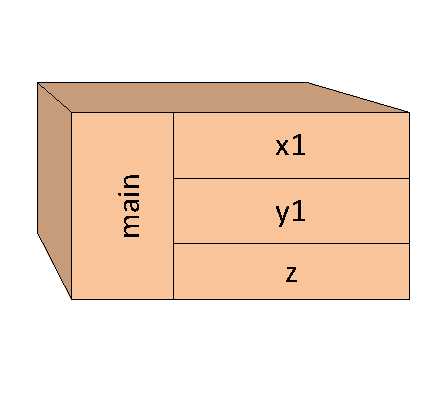
\includegraphics[scale=0.5]{../../Pictures/stack1}
	\end{center}
	\caption{Etat de la stack � l'entr�e du main}
	\label{fig:stack1}
\end{figure}

\begin{figure}[]
	\begin{center}
		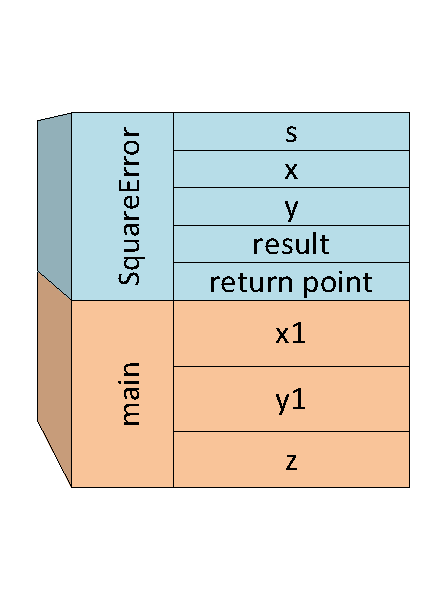
\includegraphics[scale=0.5]{../../Pictures/stack3}
	\end{center}
	\caption{Etat de la stack � l'entr�e dans SquareError}
	\label{fig:stack3}
\end{figure}

Dans cet exemple, les variables \varname{x1} et \varname{y1} sont des variables locales de la fonction \functionname{main}, tout comme les variables \varname{x} et \varname{y} sont des arguments de la fonction \functionname{SquareError}. Dans les deux cas, ces variables sont des variables muettes,  c'est � dire qu'elles servent � d�finir le sens des fonctions \functionname{SquareError} et \functionname{main}, mais qu'elles ne poss�dent pas de sens en dehors, tout comme la variable k sert � d�finir la valeur de la fonction f dans $f(n) = \sum_{k=1}^{n}\frac{1}{k^2}$. Leur scope ne se rencontrant pas, il est donc possible d'utiliser les m�mes noms de variables dans chacune des fonctions sans que cel� n'interf�re avec le sens du code. Ainsi, le code suivant donne exactement les m�mes r�sultats : \\

\begin{DDbox}{\linewidth}\begin{lstlisting}
double SquareError(double x, double y)
{
    double s = x-y;
    double result = s*s;
    return result;

}

void main()
{
    double x = 2.3;
    double y = 3.2;
    double z = SquareError(x, y);
}
\end{lstlisting}\end{DDbox}

Consid�rons un autre exemple :\\

\begin{DDbox}{\linewidth}\begin{lstlisting}

#include <math.h>

double SquareError(double x, double y)
{
	double s = x-y;
	return s*s;
}

double ManhattanError(double x, double y)
{
	double s = x-y;
    double result = abs(s);
	return result;
}

void main()
{
	double a = 2.0;
	double b = 1;
	double c = 3.0;
	double d = SquareError(a,b);
	double e = ManhattanError(a,b);
}

\end{lstlisting}\end{DDbox}

Dans cet exemple, les valeurs \varname{a,b,c,d,e} ont pour scope la fonction main. Une variable \varname{s} est d�clar�e dans \functionname{SquareError}, et elle est d�truite � la fin de la fonction. L'identifiant \varname{s} est "recycl�" dans la fonction ManhattanError, et la variable \varname{s} est �galement d�truite � la fin de cette fonction. Le double usage de l'identifiant \varname{s} ne pose pas de probl�me au compilateur, qui comprend que la variable est "muette" dans les deux cas.\\

A l'entr�e de la fonction main, l'�tat de la Stack est repr�sent� dans le graphique \ref{fig:stack4}. Lorsque la fonction \functionname{SquareError} est appel�e, la Stack se trouve dans l'�tat repr�sent� par le graphique \ref{fig:stack5}. Lorsque la fonction \functionname{SquareError} est achev�e, l'�tat de la Stack revient � celui du graphique \ref{fig:stack4}. Ensuite, la fonction \functionname{ManhattanError} est appel�e, et la Stack passe alors dans l'�tat repr�sent� dans le graphique \ref{fig:stack6}. Enfin, juste avant la fin de la fonction \functionname{ManhattanError}, et avant de retourner dans le mail, il est fait appel � la fonction \functionname{abs} qui vient ajouter alors une Stack Frame dans la Stack\footnote{Pour �tre tout � fait exact, le compilateur est capable, dans de nombreux cas comme celui-ci, de d�terminer qu'il n'est pas n�cessaire de garder trace de la Stack Frame de \functionname{ManhattanError} lorsque nous sommes dans la fonction \functionname{abs}, et qu'il peut optimiser les appels pour ne garder que les Stacks Frames de \functionname{abs} et \functionname{main} : c'est le principe du "Tail Call Optimization".}, comme il est pr�sent� dans le graphe \ref{fig:stack7}.\\

Notez que pour utiliser la fonction valeur absolue, fonction standard du langage, nous devons utiliser la librairie "math", dont les m�thodes sont d�clar�es dans le fichier header \varname{math.h} qui est stock� dans le r�pertoire de Visual Studio. Pour utiliser cette librairie, nous utilisons donc un include, mais substituons les symboles < et > en lieu et place des guillemets "" pour sp�cifier au compilateur que ce fichier \varname{math.h} appartient � la biblioth�que standard et n'est pas un fichier de votre propre cru.\\

\begin{figure}[]
	\begin{center}
		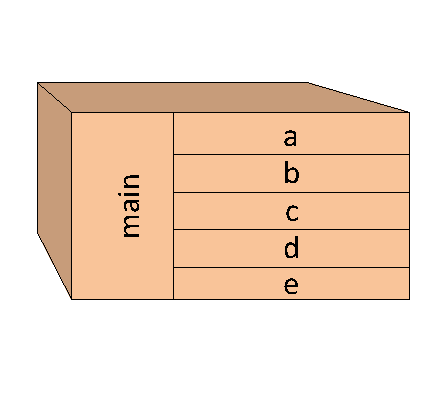
\includegraphics[scale=0.5]{../../Pictures/stack4}
	\end{center}
	\caption{Etat de la stack � l'entr�e du main}
	\label{fig:stack4}
\end{figure}

\begin{figure}[]
	\begin{center}
		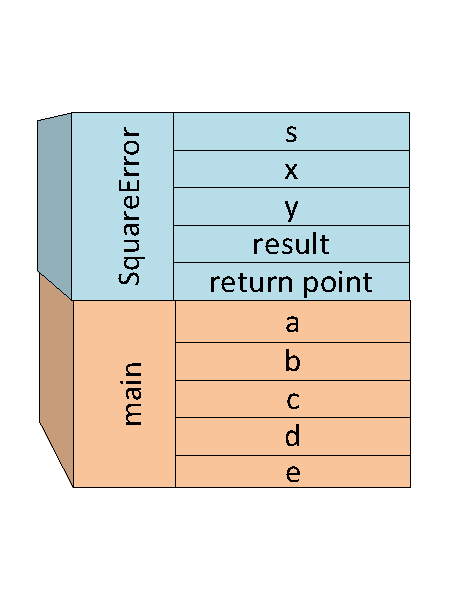
\includegraphics[scale=0.5]{../../Pictures/stack5}
	\end{center}
	\caption{Etat de la stack � l'entr�e dans SquareError}
	\label{fig:stack5}
\end{figure}

\begin{figure}[]
	\begin{center}
		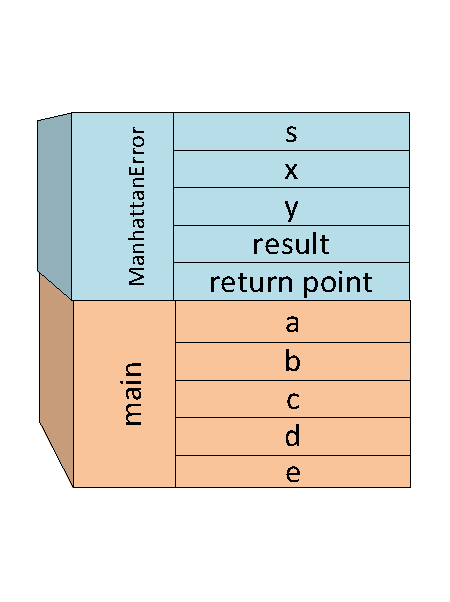
\includegraphics[scale=0.5]{../../Pictures/stack6}
	\end{center}
	\caption{Etat de la stack � l'entr�e dans ManhattanError}
	\label{fig:stack6}
\end{figure}

\begin{figure}[]
	\begin{center}
		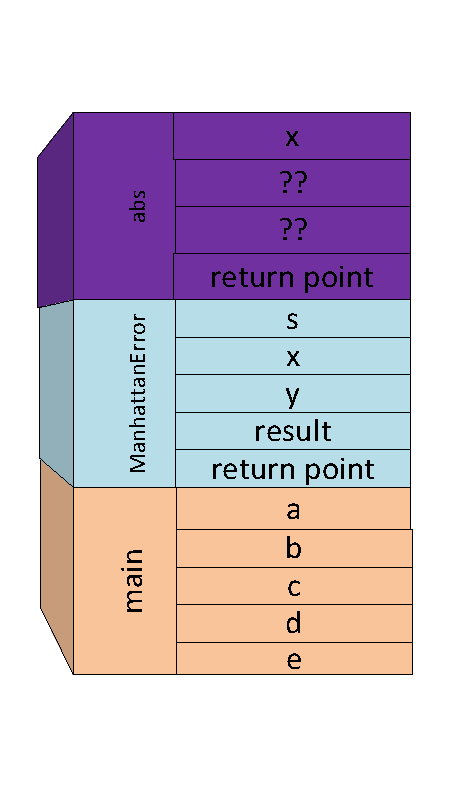
\includegraphics[scale=0.5]{../../Pictures/stack7}
	\end{center}
	\caption{Etat de la stack � l'entr�e dans abs}
	\label{fig:stack7}
\end{figure}

\section{Passage d'arguments}

Consid�rons une m�thode Increment qui prenne un entier et l'incr�mente. Nous voulons (� titre purement illustratif) que cette m�thode ne retourne pas la valeur incr�ment�e, mais qu'elle modifie directement la valeur de l'argument qui lui est pass�.

\subsection{Passage d'argument par valeur}

Une premi�re id�e serait d'impl�mententer la fonction Increment comme suit :\\

\begin{DDbox}{\linewidth}\begin{lstlisting}
void Increment1(unsigned int a)
{
    a++;
}

void main()
{
    unsigned int i = 2;
    Increment1(i);
    unsigned int b = i;
}
\end{lstlisting}\end{DDbox}

Si nous ex\'ecutons ce dernier code \footnote{Il est fortement recommand\'e
de le faire pour vous en persuader.}, nous constatons que lorsque nous appelons cette fonction dans notre main, nous n'obtenons pas les r�sultats attendus, la variable b prenant la valeur 2. La
raison \`a cela est que c'est une \emph{copie} de \texttt{i} qui est pass\'ee
\`a la fonction (copie d�sign�e par le symbole a), et non la variable i "elle-m\^eme" : le compilateur C++ va par d�faut r�aliser des copies des arguments que nous donnons � une fonction. Dans l'exemple pr�c�dent, une variable i est cr��e dans la fonction main. Lorsque nous appelons la fonction Increment1, une variable a est cr��e et le compilateur lui affecte la valeur de i. Cette valeur a est incr�ment�e dans la fonction Increment1, puis est d�truite � la fin de la fonction. Lorsque nous retournons dans la fonction main apr�s ex�cution de la fonction Increment1, nous avons donc incr�ment� une variable a, que nous avons d�truite � la fin de la fonction Increment1 et nous disposons maintenant de la variable i dont la valeur n'a jamais �t� modifi�e. \\

Exemple d'allocation m�moire avant d'entrer dans la fonction Increment1 :

\begin{center}
\begin{tabular}{l|l|l|l|l|l|l|l|l|l|l|l|l|l}
Case m\'emoire & 0 & 1 & 2 & 3 & 4 & 5 & 6 & 7 & 8 & 9 & 10 & 11 & 12 \\
\hline
Nom &  &  & i  & i  & i & i &  & &  & & & & \\
\hline
Valeur &  &  & 0100... & 000... & 00...  & 000... &  &  &  &  &  &  & \\
\end{tabular}
\end{center}

En entrant dans la fonction Increment1 :

\begin{center}
\begin{tabular}{l|l|l|l|l|l|l|l|l|l|l|l}
Case m\'emoire & 0 & 1 & 2 & 3 & 4 & 5 & 6 & 7 & 8 & 9 & 10  \\
\hline
Nom &  &  & i  & i  & i & i &  & a & a & a & a \\
\hline
Valeur &  &  & 0100... & 000... & 00...  & 000.. &  &0100... & 000... & 00...  & 000..  \\
\end{tabular}
\end{center}

Juste avant de sortir de la fonction Increment1 :

\begin{center}
\begin{tabular}{l|l|l|l|l|l|l|l|l|l|l|l}
Case m\'emoire & 0 & 1 & 2 & 3 & 4 & 5 & 6 & 7 & 8 & 9 & 10  \\
\hline
Nom &  &  & i  & i  & i & i &  & a & a & a & a \\
\hline
Valeur &  &  & 0100... & 000... & 00...  & 000.. & & 1100... & 000... & 00...  & 000.. \\
\end{tabular}
\end{center}

De retour dans le main apr�s appel � Increment1 :

\begin{center}
\begin{tabular}{l|l|l|l|l|l|l|l|l|l|l|l}
Case m\'emoire & 0 & 1 & 2 & 3 & 4 & 5 & 6 & 7 & 8 & 9 & 10  \\
\hline
Nom &  &  & i  & i  & i & i &  & &  & &  \\
\hline
Valeur &  &  & 0100... & 000... & 00...  & 000.. &  &  &  &  &  \\
\end{tabular}
\end{center}

Il nous faut �galement sp�cifier en C++ au compilateur que nous ne voulons pas qu'il travaille avec une copie de la variable i, mais bien avec la variable i elle-m�me.

\subsection{Passage d'argument par pointeur}

Reprenons l'exemple pr�c�dent avec des pointeurs :\\

\begin{DDbox}{\linewidth}\begin{lstlisting}
void Increment2(int* p)
{
    (*p)++;
}

void main()
{
    int i = 2;
    int* pi = &n;
    Increment2(pi);
    int b = i;
}
\end{lstlisting}\end{DDbox}

Cette fois-ci, nous avons donn� en argument non pas la variable i, mais un pointeur vers cette variable i via la variable pointeur pi. Le compilateur va cr�er une copie de la variable pi, p, qui prendra la m�me valeur que pi, c'est � dire qui pointera sur i �galement. Lorsque nous ex�cutons le code de la fonction Increment2, nous acc�dons donc bien � l'adresse m�moire de la variable i, qui est effectivement modifi�e.

\subsection{Passage d'argument par r�f�rence}
Le C++ (� la diff�rence du C), propose un sucre syntaxique pour abstraire la manipulation de pointeur : c'est le passage par r�f�rence. Plus pr\'ecis\'ement, il existe un \'equivalent du \texttt{ByRef} de Visual
 Basic, qui est le signe \&. Lorsque nous passons une valeur par r�f�rence, nous adoptons la syntaxe du passage par valeur (au symbole \& pr�t) mais le compilateur va interpr�ter ceci comme un passage par pointeur. En voici un exemple :\\

\begin{DDbox}{\linewidth}\begin{lstlisting}
void Increment3(int& a)
{
    a++;
}
void main()
{
    int a = 2;
    Increment3(a);
    int b = a;
}
\end{lstlisting}\end{DDbox}

Nous obtenons bien une valeur de 3 pour la variable b � la fin du main.\\

\begin{warning}
Il est important de noter que
 l'emploi du signe \& \`a c\^ot\'e d'une d\'eclaration de variable n'a
 \emph{pas} le m�me sens que celui de l'op\'erateur qui r\'ecup\`ere l'adresse
 m\'emoire d'un objet. Il y a donc 2 sens diff�rents � la fois pour les op�rateurs \& et *.\\
\end{warning}

Il y a deux raisons pour lesquelles nous pouvons souhaiter passer un argument par r�f�rence :
\begin{itemize}
\item La premi�re, comme nous venons de le voir, pour modifier r�ellement la valeur de l'argument en dehors de la fonction appel�e.
\item La deuxi�me, pour �viter une copie (copie qui aurait des cons�quences en termes de co�t et de sens).
\end{itemize}

Dans le deuxi�me cas, puisque c'est vraiment l'objet et non pas une copie de lui-m�me qui est pass� � la fonction, la fonction pourrait donc modifier par inadvertance l'objet donn� en argument. Nous souhaiterions parfois pouvoir interdire la modification de l'objet manipul�, par mesure de s�curit�, lorsque celui-ci est donn� en argument par r�f�rence. Le C++ permet de faire ceci en pr�cisant au niveau de l'argument de la fonction que celui-ci est constant (immutable) et qu'il ne devra pas �tre modifi� :\\

\begin{DDbox}{\linewidth}\begin{lstlisting}
void WidgetFunction(const int& a)
{
    //Do something
}
\end{lstlisting}\end{DDbox}

Dans notre cas d'incr�mentation, nous ne souhaitons bien �videmment pas que la fonction Increment3 utilise un argument immutable comme dans l'exemple pr�c�dent, puisque pr�cis�ment le but de la fonction est de modifier l'argument. Si cependant nous nous y essayions, le compilateur retournerait une erreur, car il est capable de d�tecter statiquement (c'est � dire � la compilation et non � l'ex�cution) que le code essaye de modifier une variable d�finie comme immutable.

\section{Effets de bord}

Le fait qu'une fonction agisse non pas par sa valeur de retour mais par le fait qu'elle modifie un de ses arguments, comme c'�tait le cas dans notre m�thode Increment3 au dessus, est appel� effet de bord. En r�gle g�n�rale, les effets de bord sont peu intuitifs et doivent �tre utilis�s avec circonspection.

\begin{habitudes}[M�thodes � effet de bord]

Lorsqu'une m�thode a des effets de bord, il est de bon go�t que cette m�thode n'ait pas de type de retour. Ainsi, il est beaucoup plus ais� au relecteur du code de deviner que la m�thode va agir par effet de bord. Inversement, une m�thode qui a un type de retour n'est pas sens�e avoir des effets de bord sur ses arguments.

\end{habitudes}

\begin{savequote}
--- Knowing C is a prerequisite for learning C++, right?\\

Wrong. The common subset of C and C++ is easier to learn than C. There will be
less type errors to catch manually (the C++ type system is stricter and more
expressive), fewer tricks to learn (C++ allows you to express more things
without circumlocution), and better libraries available.  The best initial
subset of C++ to learn is not "all of C".  Bjarne Stroustrup, FAQ sur
sa page personnelle \end{savequote}

\chapter{Autres \'el\'ements de syntaxe }
\label{chapter:elementsdesyntaxe}

\section{Boucles et tests de condition}
\subsection{Tests}
\subsubsection{Tests simples}

Comme dans les autres langages, nous voulons pouvoir faire des tests
sur les valeurs des variables. La syntaxe d'un test ainsi qu'un exemple peuvent \^etre lus ci-dessous:\\

\begin{DDbox}{\linewidth}
\begin{minipage}{0.45\linewidth}
    \begin{lstlisting}[caption=Syntaxe d'un test]

    if (condition)
    {
        /*Code*/
    }
    else if(condition)
    {
        /*Code*/
    }
    else
    {
    ...
    }

    \end{lstlisting}
\end{minipage}
\qquad
\begin{minipage}{0.45\linewidth}
    \begin{lstlisting}[caption=Exemple de test]

    if (0 == x)
    {
        x = x + 1;
    }
    else if (1 == x)
    {
       x = x * 2;
    }
    else
    {
       x = x + 3;
    }

    \end{lstlisting}
\end{minipage}
\end{DDbox}

Nous pouvons \'egalement noter dans l'exemple l'utilisation de \texttt{==} pour
effectuer un test d'\'egalit\'e. Le test de diff\'erence se fait \`a l'aide de
l'op\'erateur \verb+!=+.\\

\begin{warning}
Le code suivant, bien que valide syntaxiquement, ne fait pas ce qui est attendu :\\
\end{warning}

\begin{DDbox}{\linewidth}
\begin{lstlisting}[caption=Une erreur classique, label=erreuraffectation]
if (x = 0)
{
    x = x + 1;
}
\end{lstlisting}
\end{DDbox}

En effet, il manque un symbole "=" dans le test du if. Le code en question va donc mettre
la valeur 0 dans la variable x, avec des r\'esultats impr\'evisibles pour la suite.

\begin{habitudes}[Test]

Afin d'\'eviter l'erreur classique du listing \ref{erreuraffectation}, une bonne habitude est d'inverser les param\`etres du test:\\

\begin{DDbox}{\linewidth}
\begin{lstlisting}
if (0 == x)
{
	x =  x + 1
}
\end{lstlisting}
\end{DDbox}

En lieu et place de :\\

\begin{DDbox}{\linewidth}\begin{lstlisting}
if (x == 0)
{
	x =  x + 1
}
\end{lstlisting}
\end{DDbox}

\end{habitudes}

Enfin, nous remarquons \`a nouveau l'emploi des accolades pour signifier le
d\'ebut et la fin d'un bloc logique (comme en Java). Les habitu\'es de
Python noteront que l'indentation est libre - contrairement \`a Python -, ce
qui justifie l'emploi des accolades\footnote{Une petite pr\'ecision est \`a apporter : dans le cas o\`u le code conditionnel à ex\'ecuter fait une seule ligne, on peut se passer des accolades.  Cependant, cette pratique est dangereuse (on rajoute une ligne apr\`es et l'on oublie de rajouter les accolades) et donc \`a \'eviter au moins dans un premier temps.}.

\begin{habitudes}[Indentation]
Il est \emph{tr\`es} important d'indenter son code correctement, faute de quoi il devient rapidement illisible.
\end{habitudes}

\subsubsection{Tests en s\'eries}
Il arrive parfois que l'on cherche \`a effectuer une s\'erie de tests, comme sur le listing \ref{lst:testserielaid.cpp}.\\

\includecodecaption{testserielaid.cpp}{Tests en s\'erie}

Ecrire la s\'erie de test de cette mani\`ere n'est pas tr\`es \'el\'egante. Le langage C++ fournit une construction particuli\`ere, appel\'ee \keyword{switch}.
La syntaxe est la suivante:\\

\begin{DDbox}{\linewidth}
\begin{minipage}{0.45\linewidth}
    \begin{lstlisting}[caption=Syntaxe d'un switch]

switch (variable)
{
    case valeur1 :
    	/*code*/
	   break;
    case valeur2 :
    	/*code*/
	   break;
    /*autres cas*/
    default:
       /*code*/
       break;
}
    \end{lstlisting}
\end{minipage}
\qquad
\begin{minipage}{0.45\linewidth}
    \begin{lstlisting}[caption=Exemple de tests multiples]
switch(c)
{
	case 'A':
		cout << ``lettre A'';
		break;
	case 'B':
		cout << ``lettre B'';
		break;
	default:
		cout <<``Autre lettre'';
        break;
}

    \end{lstlisting}
\end{minipage}
\end{DDbox}

\begin{itemize}
		
	\item  Le mot cl\'e \keyword{switch} indique que nous allons op\'erer une
		s\'eparation des cas.
		
	\item   Chaque cas est ensuite trait\'e \`a l'aide du mot cl\'e
		\keyword{case}.

	\item Les cas non pr\'evus explicitement sont trait\'es par le cas
		\keyword{default}.

	\item Le mot cl\'e \keyword{break} sert \`a indiquer la fin du cas. Si
		ce mot cl\'e est absent, le cas en dessous sera
		\emph{\'egalement ex\'ecut\'e}.
		
\end{itemize}



Le code du listing \ref{lst:testserielaid.cpp} devient donc :\\

\includecodecaption{testserieswitch.cpp}{Tests en s\'erie}


Le code obtenu pr\'esente l'avantage d'\^etre beaucoup plus clair et \'el\'egant qu'avant.

\subsection{Boucles}

\subsubsection{La boucle \keyword{for}}

Fr\'equemment, nous nous retrouvons dans une situation o\`u
nous souhaitons parcourir un tableau ou une liste, ou encore parcourir le
nombres de 1 \`a 100 pour pouvoir les afficher.  On retrouve en C++ comme ailleurs la boucle \verb+for+, dont la forme g\'en\'erale est :\\

\begin{DDbox}{\linewidth}
\begin{lstlisting}[caption=Syntaxe d'une boucle \texttt{for}]
for(variable1,variable2,...= valeurs de depart;
    condition de terminaison;
    operation sur les variables)
{
    /*Code*/
}

\end{lstlisting}
\end{DDbox}

Par exemple, pour \'enum\'erer et afficher les nombres de 1 \`a 100 nous \'ecririons le code suivant:\\

\begin{DDbox}{\linewidth}
\begin{lstlisting}[caption=Exemple de boucle \texttt{for}]

for(int i = 1 ; i <= 100; i++) /*i++ signifie i=i+1*/
{
    cout << i << endl;
    //Note : endl signifie retour a la ligne
}
\end{lstlisting}
\end{DDbox}

\subsubsection{La boucle \keyword{while}}

L'autre type de boucle dont nous pouvons avoir besoin est une boucle signifiant \textit{tant que}, que nous exprimons \`a l'aide du mot cl\'e \keyword{while}. La condition est test\'ee \emph{avant} le bloc de code.\\

\begin{DDbox}{\linewidth}
\begin{lstlisting}
while (condition)
{
    /*code*/
}
\end{lstlisting}
\end{DDbox}

L'affichage des nombres de 1 \`a 100 s'\'ecrirait donc :\\

\begin{DDbox}{\linewidth}
\begin{lstlisting}[label=lst:whileexample]
int i=1; /*on peut initialiser une variable*/

while ( i <= 100 )
{
    cout << i << endl;
    i++;
}
\end{lstlisting}
\end{DDbox}

Ce type de boucle pr\'esente \'egalement une variante, dans laquelle la condition de sortie se trouve \`a la fin:\\

\begin{DDbox}{\linewidth}
\begin{lstlisting}
do
{
	/*code*/
}
while(condition);
\end{lstlisting}
\end{DDbox}

Le listing \ref{lst:whileexample} devient donc:\\

\begin{DDbox}{\linewidth}
\begin{lstlisting}
int i=0; /*on peut initialiser une variable*/

do
{
    i++;
    cout << i << endl;
}
while ( i < 100 )
\end{lstlisting}
\end{DDbox}

Dans cette variante, l'int\'erieur des brackets est ex\'ecut\'e au moins une fois, quoi qu'il arrive.\\

\subsubsection{\keyword{break} et \keyword{continue}}
Nous avons parfois besoin d'interrompre l'ex\'ecution d'une boucle, ou de sauter une \'etape lors de son ex\'ecution. C'est le r\^ole des mots cl\'es \keyword{break} et \keyword{continue}.\\

\keyword{break} sert \`a interrompre l'ex\'ecution d'une boucle, comme dans l'exemple suivant :\\

\includecode{examplebreak.cpp}
%qui donne la sortie suivante:\\
%\verbatiminput{code/examplebreak.out}

\keyword{continue} sert \`a sauter l'\'etape courante de la boucle. Par exemple, pour afficher les nombres pairs entre 1 et 10, nous pourrions \'ecrire :\\

\includecode{examplecontinue.cpp}
%qui donne la sortie suivante:\\
%\verbatiminput{code/examplecontinue.out}

%\begin{savequote}
Object-oriented programming is an exceptionally bad idea which could only have originated in California.
\qauthor{propos pr�t� faussement � Edsger Dijkstra, r�el auteur inconnu}
\end{savequote}

\chapter{Les templates}

Les templates sont un m\'ecanisme puissant de factorisation de code, qui permettent d'\'ecrire du code g\'en\'erique s'appliquant \`a des donn\'ees,
ind\'ependamment de leur type. Plus pr\'ecis\'ement, ils permettent de produire en un seul fichier une famille de fonctions ou une famille de
classes indic\'ees par un type abstrait ou par un autre param\`etre comme un entier.\\

\section{Templating par un type, l'exemple des fonctions}

Les templates sont issus originellement d'un souci de simplification de code par la factorisation, afin d'\'eviter les redondances. Prenons
l'exemple d'une fonction Max qui prenne en argument un tableau de double et la taille de ce tableau :\\

\begin{DDbox}{\linewidth}
\begin{lstlisting}
double Max(double array[], int length)
{
    double vmax = array[0];
    for (int i = 1; i < length; i++)
        if (array[i] > vmax)
            vmax = array[i];
    return vmax;
}
\end{lstlisting}
\end{DDbox}

Si nous voulions d\'efinir la m\^eme fonction sur un tableau d'entiers, nous devrions alors produire le code suivant : \\

\begin{DDbox}{\linewidth}
\begin{lstlisting}
int Max(int array[], int length)
{
    int vmax = array[0];
    for (int i = 1; i < length; i++)
        if (array[i] > vmax)
            vmax = array[i];
    return vmax;
}
\end{lstlisting}
\end{DDbox}

De la m\^eme mani\`ere, nous pourrions d\'efinir la fonction Max sur un tableau de float, de ushort, de uint, de long, etc... Dans le cadre
d'exemples plus complexes, le d\'edoublement du code pour chaque type est tr\`es p\'enalisant : tout d'abord, il nuit \`a la clart\'e du code pour
le lecteur, mais il entraine aussi un risque important de divergence des diff\'erentes versions du code. En effet, si la s\'emantique de la fonction
Max est incorrecte, elle le sera \`a la fois pour la version du code manipulant des entiers comme pour celle manipulant des doubles. Si un
d\'eveloppeur est amen\'e \`a am\'eliorer ou d\'ebugger une version de cette fonction, il court le risque d'oublier que d'autres versions de cette
fonction demandent probablement les m\^emes modifications.\\

Nous le concevons donc, \textbf{la redondance du code est \`a proscrire}\footnote{La r\`egle 1 du d\'eveloppement pourrait \^etre : "ne faites pas
de copier/coller de code au sein d'un projet."}. Comment dans ces conditions cr\'eer une seule fonction Max qui permette de d\'efinir cette fonction
pour des entiers, mais aussi pour des double, des uint, etc... ? Le C++ propose un m\'ecanisme pour d\'efinir en une fois le code devant
s'appliquer, quel que soit le type des arguments. Observons la syntaxe suivante : \\

\begin{DDbox}{\linewidth}
\begin{lstlisting}
template<typename T>
T Max(T array[], int length)
{
    T vmax = array[0];
    for (int i = 1; i < length; i++)
        if (array[i] > vmax)
            vmax = array[i];
    return vmax;
}
\end{lstlisting}
\end{DDbox}

Dans cet exemple, la fonction Max devient param\'etr\'ee par un type abstrait T. Celui-ci est utilis\'e dans notre exemple \`a la fois pour
d\'efinir le type du premier argument de la fonction, mais \'egalement pour d\'efinir son type de retour. Le pr\'efixe template<typename T> indique
au compilateur que le code qui suit sera param\'etr\'e par un type T. De mani\`ere \'equivalente, le mot clef \textit{typename} peut \^etre
remplac\'e par \textit{class}.\\

Lorsque dans notre code, nous voulons utiliser notre fonction Max, nous pouvons le faire de la sorte :\\

\begin{DDbox}{\linewidth}
\begin{lstlisting}
int values[]={ 16, 8, 3, 2, 11 };

cout << Max<int>(values, 5);
\end{lstlisting}
\end{DDbox}

Lorsque le compilateur va lire l'appel \`a Max(values, 5), il va d\'etecter qu'il s'agit d'utiliser la fonction templat\'ee Max dans le cas o\`u T =
int. Le compilateur va alors g\'en\'erer le code correspondant et l'inclure dans la compilation. Bien \'evidemment, le compilateur ne g\'en\`erera
la fonction Max que pour les types T pour lesquels il est fait appel quelque part \`a la fonction Max utilis\'ee pour le type T : si nulle part dans
notre code nous ne cherchons \`a d\'eterminer le max d'un tableau de double, le code sp\'ecifique pour la fonction Max en le type double ne sera pas
g\'en\'er\'e.\\

Le fait d'utiliser une fonction templat\'ee en un type sp\'ecifique est appel\'e \textit{sp\'ecialisation}. Pouvons-nous sp\'ecialiser la fonction
Max en n'importe quel type ? L'approche du C++ sur la question est une approche optimiste (\`a la diff\'erence du C\# par exemple) : par d\'efaut,
tout type est accept\'e. C'est uniquement \`a la compilation que le compilateur va tenter de g\'en\'erer le code n\'ecessaire pour chacun des types
en lesquels la fonction templat\'ee a \'et\'e sp\'ecialis\'ee. Si notre fonction est sp\'ecialis\'ee en un type T1 pour lequel l'op\'erateur < n'est
pas d\'efini, alors le compilateur \'echouera dans la g\'en\'eration du code sp\'ecialis\'e.\\

\subsection{Templates et macro}

Si nous reprenons la fonction templat\'ee pr\'ec\'edente appliqu\'ee \`a deux valeurs plut\^ot qu'\`a un tableau, nous pouvons produire le code
suivant :\\

\begin{DDbox}{\linewidth}
\begin{lstlisting}
template<typename T>
const T & Max( const T & a, const T & b )
{
    return a > b ? a : b;
}
\end{lstlisting}
\end{DDbox}

Cet exemple ressemble beaucoup avec la macro correspondante, comme d\'etaill\'ee dans le chapitre sur la compilation :\\

\begin{DDbox}{\linewidth}
\begin{lstlisting}
#define MAX(a, b) (((a) > (b)) ? (a) : (b))
\end{lstlisting}
\end{DDbox}

En effet, dans chaque cas, nous avons une impl\'ementation de la fonction max qui peut s'adapter \`a tous types d'objets. Le templating est la
mani\`ere propre d'\'ecrire des macros. L\`a o\`u la macro est une simple substitution syntaxique, avec toutes les erreurs qui en d\'ecoulent
(\ref{sec:macros}), le templating g\'en\`ere de r\'eelles fonctions et permet donc d'obtenir de mani\`ere fiable le r\'esultat.\\

Dans la comparaison qui vient d'\^etre faite, il faut noter cependant qu'un avantage majeur de la macro par rapport \`a son homologue templat\'ee
est l'absence d'appel de fonction : puisque la macro ne cr\'ee pas de v\'eritable fonction, il n'y a pas d'appel de fonction et donc pas de co\^ut
d'appel de fonction. Il est possible d'\'eviter ce co\^ut \'egalement dans le cas d'une fonction templat\'ee, en l'inlinant :\\

\begin{DDbox}{\linewidth}
\begin{lstlisting}
template<typename T>
inline const T & Max( const T & a, const T & b )
{
    return a > b ? a : b;
}
\end{lstlisting}
\end{DDbox}

\subsection{Fonctions membres templat\'ees}

Il est \'egalement possible de cr\'eer une fonction templat\'ee au sein d'une classe non templat\'ee. L'exemple suivant d\'ecrit une classe
disposant d'une fonction membre templat\'ee permettant d'afficher diff\'erente objets.\\

\begin{DDbox}{\linewidth}
\begin{lstlisting}
class SomeClass
{
    public SomeClass();
    public ~SomeClass();

    template<typename T>
    static void Display( const T & t )
    {
        cout << t;
    }
}

int main()
{
    SomeClass.Display<int>(2);
    SomeClass.Display<string>("Hello World");
    SomeClass.Display<double>(3.14);
}
\end{lstlisting}
\end{DDbox}

\subsection{Inf\'erence automatique de type de sp\'ecialisation}

Lorsque le compilateur est capable d'inf\'erer le type en lequel est sp\'ecialis\'ee une fonction templat\'ee, il est superflu de sp\'ecifier
explicitement en quel type la fonction est sp\'ecialis\'ee. Dans le cas du code pr\'ec\'edent par exemple, nous pourrions \'ecrire :\\

\begin{DDbox}{\linewidth}
\begin{lstlisting}
int main()
{
    SomeClass.Display(2);
    SomeClass.Display("Hello World");
    SomeClass.Display(3.14);
}
\end{lstlisting}
\end{DDbox}

Il est cependant des cas o\`u une telle inf\'erence n'est pas possible, notamment dans le cas d'ambigu\"it\'e que le compilateur ne peut pas lever
lui-m\^eme. Ainsi, la fonction suivante doit \^etre sp\'ecifi\'ee explicitement :\\

\begin{DDbox}{\linewidth}
\begin{lstlisting}
template <typename T>
T Sum( T s1, T s2 )
{
    return s1 + s2;
}

int main()
{
    int s2 = 1;
    double s1 = 3.2;

    Sum( s1, s2 ); // Erreur : paramètre ambigü
    Sum<double>( s1, s2 ); // OK
}
\end{lstlisting}
\end{DDbox}

\subsection{Multi-templating}

Il est possible de param\'etrer une fonction par plusieurs arguments; en voici un exemple :\\

\begin{DDbox}{\linewidth}
\begin{lstlisting}
template<typename T, typename U>
public T Add (const T& t, const U& u)
{
    return t+u;
}
\end{lstlisting}
\end{DDbox}

\section{Templating par un type, le cas des classes}

De la m�me mani�re que nous avons d�fini le param�trage d'une fonction par un type g�n�rique T, nous pouvons param�trer une classe par un type g�n�rique.  Le templating par des classes est principalement utilis� pour construire des "containers", c'est � dire des classes dont la fonction est de contenir un ensemble d'�l�ments d'un m�me type. Un exemple �clairant sera donn� dans la section \ref{subsection:VectorCode}.

\section{Templates et compilation}

Un voile pudique est bien souvent jet� par les manuels d'introduction au C++ sur la compilation des templates. Ceux-ci r�pondant � des contraintes bien particuli�res (puisqu'il ne s'agit pas de code mais de "m�ta-code"), il n'est pas possible par d�faut de d�clarer une fonction template dans un fichier .h puis de la d�finir dans un fichier .cpp. Par d�faut, il vous faudra donc m�langer d�claration et d�finition dans un m�me fichier .h sous peine de vous exposer � des erreurs � l'�dition des liens. Comme il est expliqu� dans l'article d'Aur�lien Regat-Barrel sur le site cpp.developpez.com, il existe n�anmoins une astuce permettant de contourner le probl�me.\\

Cette astuce consiste � stocker la d�claration de votre classe templat�e dans un fichier .h, de stocker votre d�finition dans un fichier texte (avec une extension diff�rente de .cpp, comme .tpp par exemple), et d'inclure gr�ce � l'instruction \#include le fichier .tpp � la fin du fichier header. Ainsi, nous obtenons par exemple quelquechose de la forme : \\

\begin{DDbox}{\linewidth}
\begin{lstlisting}
// exemple.h

#ifndef EXEMPLE_H
#define EXEMPLE_H

template <typename T>
class Exemple
{
public:
    Exemple();
};

#include "exemple.tpp" // voici l'astuce
#endif

// exemple.tpp

template <typename T>
Exemple<T>::Exemple()
{
}

\end{lstlisting}
\end{DDbox}

\section{Templates et sp�cialisation}

Il existe certains cas o� nous voudrions faire des exceptions � la g�n�ricit�, c'est � dire que pour certains types bien particuliers, une fonction templat�e ait un comportement particulier, qui diff�re du comportement g�n�ral d�j� d�fini. Prenons le cas de l'exponentiation de 2. Si $y$ est un r�el (double ou float), le calcul de $2^{y}$ demande de r��crire la formule en $e^{y.ln(2)}$ afin de l'�valuer. Nous pourrions donc �crire :\\

\begin{DDbox}{\linewidth}
\begin{lstlisting}

template<typename T>
double TwoPow(T y)
{
    return exp(y*ln(2);
}
\end{lstlisting}
\end{DDbox}

Cette fonction fonctionnerait �galement si elle �tait sp�cifi�e en deux entiers. Cependant, dans le cas o� y est entier, il n'est pas n�cessaire de passer par cette formule, il suffit alors de multiplier 2 par lui m�me y fois. Bien que la formule pr�c�dente soit exacte dans le cas o� y est entier, elle entrainerait donc des calculs ind�ment longs. Pour am�liorer cette situation, nous voudrions dire au compilateur : compile la fonction pr�c�dente pour tous les types n�cessaires, SAUF dans le cas o� y est entier, auquel cas contente toi de calculer directement la valeur de l'exponentiation. En C++, il est possible de pr�ciser/red�finir une sp�cialisation sp�cifique.\\

\begin{DDbox}{\linewidth}
\begin{lstlisting}

// Sp�cialisation pour les int
template <>
double TwoPow<int>( int i )
{
    double q= (i >= 0) ? 2 : 0.5;
    int iAbs = abs(i);
    double r=1;

    for (int j = 0 ; j < iAbs;j++)
        r*=q;

    return r;
}

\end{lstlisting}
\end{DDbox}

\subsection{Sp�cialisation partielle}

Les templates peuvent �tre partiellement sp�cialis�s, et la classe obtenue est alors encore un template. Cette sp�cialisation partielle intervient principalement dans le cas dans le cas d'un template param�tr� par plusieurs types, pour lesquels seuls certains de ces types sont sp�cialis�s, le r�sultat �tant un template param�tr� dans les types restants. Exemple :\\

\begin{DDbox}{\linewidth}
\begin{lstlisting}
template<typename T, typename U>
public double Pow(T x, U y)
{
    return exp(y*ln(x));
}

template<typename T>
public double Pow<T,int>(T x, int y)
{
    double q= (y >= 0) ? x : ((double)1)/x; //do not forget the explicit cast into double !
    int yAbs = abs(y);
    double r=1;

    for (int j = 0 ; j < yAbs;j++)
        r*=q;

    return r;
}
\end{lstlisting}
\end{DDbox}

\section{Templating par des entiers}

Il est �galement possible de param�trer une fonction par autre chose qu'un type. Notamment, il est possible de param�trer une fonction par un entier. Ces m�canismes ne seront pas d�taill�s cette ann�e, mais ils sont massivement utilis�s dans de nombreuses librairies professionnelles, car ils permettent des optimisations tr�s fines, notamment via le Template Meta-Programming. Les bonnes librairies de calcul scientifique en C++ par exemple reposent toutes massivement sur ce genre d'optimisation. Nous renvoyons le lecteur int�ress� par exemple � \cite{Alexandrescu}. 
\part{Programmation orient\'ee objet}
\begin{savequote}[80mm]
- [...] Mais c'est pas �a qu'on appelle la classe. Je te dis �a en qualit� d'homme le plus classe du monde.\\

- Eh je t'arr�te tout de suite. La classe, c�est d'�tre chic dans sa mani�re de s'habiller. Rien de tel que d'aller chez Azzedine Alaia m�me de s'acheter des sous-pulls chez Yohji Yamamoto !\\

- Excuse-moi de te dire �a mon pauvre Jos�, mais tu confonds un peu tout. Tu fais un amalgame entre la coquetterie et la classe. Tu es fou. Tu d�penses tout ton argent dans les habits et accessoires de mode mais tu es ridicule. Enfin si �a te plait... C'est toi qui les portes. Mais moi, si tu veux mon opinion, �a fait un peu... has been.\\

\qauthor{La classe am�ricaine, Jos� et Georges Abitbol}
\end{savequote}

\chapter{Introduction \`a l'objet : les classes}

La complexit� d'un code n'est pas lin�aire avec sa taille : plus un projet est volumineux, plus l'ajout marginal de code s'av�re complexe. Il devient rapidement
(au del� de quelques centaines de lignes de code) n�cessaire d'architecturer le code pour en faciliter la lecture,
et donc la maintenance et le debuggage. Cette probl�matique est devenue centrale. En effet, depuis 30 ans la taille des projets a explos� : pour maintenir un projet, il faut donc penser son architecture pour l'organiser comme une synergie d'objets ind�pendants incarnant chacun un r�le/une fonctionnalit�.\\

L'id�e fondamentale, c'est d'avoir des entit�s logiques riches, le plus distinctes, r�duites et d�coupl�es possible. Dans ce chapitre, nous introduisons ces entit�s logiques riches, appel�es classes. En r�gle g�n�rale, une classe regroupe un ensemble de donn�es et de m�thodes. L'architecture g�n�rale d'une classe est de ne rendre disponible qu'une petite partie de ses fonctions (appel�es m�thodes) et donn�es, celles r�ellement utiles de l'ext�rieur, et de cacher pour l'ext�rieur la majorit� de son impl�mentation. Cette conception permet de d�coupler les diff�rentes complexit�s d'un programme et de simplifier la lecture du code : pour comprendre comment utiliser une classe, il suffit de comprendre ce que font les m�thodes "publiques" et non pas de comprendre tous les m�canismes sous-jacents.\\

La notion de classe est si centrale qu'on d�signe souvent les langages qui permettent ce genre d'entit�s comme des langages "orient�s objet". Jusqu'� pr�sent, nous avions pr�sent� nos programmes sous une forme proc�durale, c'est � dire qu'une m�thode main appelait d'autres fonctions qui � leur tour en appelaient des autres, ... A pr�sent, nous cr�erons des objets, instances de types plus complexes, o� chaque type repr�sentera un ensemble de m�thodes et de donn�es formant une unit� logique.\\

A titre illustratif, nous utiliserons dans tout ce chapitre l'exemple d'une classe accumulator dont la fonction sera de calculer la moyenne et la variance empirique de valeurs r�elles.

\section{D�claration des classes}

Commen�ons par d�clarer une classe Accumulator. Cette classe contiendra plusieurs variables, appel�es des \textit{champs}. Voici la d�claration de cette classe dans le fichier Accumulator.h correspondant :\\

\begin{DDbox}{\linewidth}
\begin{lstlisting}
//Accumulator.h
#ifndef ACCUMULATOR_H
#define ACCUMULATOR_H

#include <string.h>

class Accumulator
{
public:
	int n;
	double xSum;
	double xSquareSum;
}; //ne pas oublier le ; ici !

#endif
\end{lstlisting}
\end{DDbox}

Les champs n, xSum et xSquareSum sont intrins�ques � la classe. Chaque instance, c'est � dire chaque exemplaire de la classe Accumulator poss�dera ces attributs.\\

Une fois notre classe d�clar�e, nous pouvons alors d�clarer des instances de ce type;
Nous d�clarons/d�finissons donc un accumulator dans notre main de la mani�re suivante :\\

\begin{DDbox}{\linewidth}
\begin{lstlisting}
//main.cpp
#include "Accumulator.h"

void main()
{
	Accumulator acc;
}

\end{lstlisting}
\end{DDbox}

Nous pouvons �crire des m�thodes reli�es � la classe Accumulator. Pour cel�, nous ajoutons dans la d�claration de
notre classe les prototypes des m�thodes que nous souhaitons ajouter :\\

\begin{DDbox}{\linewidth}
\begin{lstlisting}
//Accumulator.h
#ifndef ACCUMULATOR_H
#define ACCUMULATOR_H

class Accumulator
{
    public:
    	int n;
    	double xSum;
    	double xSquareSum;

    	void Add(double);
};

#endif
\end{lstlisting}
\end{DDbox}

Pour d�finir la m�thode correspondante, nous proc�dons comme pr�c�demment, mais pr�c�dons le nom de la m�thode du nom de la classe suivi de "::", afin de signifier au compilateur que la m�thode est attach�e � cette classe (nous parlons alors de \textit{fonction membre}).\\

\begin{DDbox}{\linewidth}
\begin{lstlisting}
//Accumulator.cpp

#include "Accumulator.h"

void Accumulator::Add(double x)
{
	n++;
    xSum += x;
    xSquareSum += x*x;
}
\end{lstlisting}
\end{DDbox}

Lorsque nous souhaitons utiliser une m�thode ou un champ d'une classe, la syntaxe que nous utiliserons sera
la suivante :\\

\begin{DDbox}{\linewidth}
\begin{lstlisting}
instance.champ = ...
instance.Method()
\end{lstlisting}
\end{DDbox}

En reprenant le code pr�c�dent, nous souhaitons maintenant calculer la moyenne des 10 premiers entiers. \\

Nous adaptons donc notre fonction main :\\

\begin{DDbox}{\linewidth}
\begin{lstlisting}
void main()
{
    //construction of object acc
    Accumulator acc;

    //Initialisation of the object
    acc.n=0;
    acc.xSum =0;
    acc.xSumQuare=0;

    for (int i = 0 ; i < 10;i++)
    {
        acc.Add( (double) i);
    }

    double mean = acc.xSum / acc.n;
}
\end{lstlisting}
\end{DDbox}

\section{Initialisation et constructeurs}

\subsection{Une premi�re m�thode d'initialisation}

L'initialisation propos�e dans la section pr�c�dente pr�sente plusieurs inconv�nients :\\

\begin{itemize}
\item elle est tr�s verbeuse, puisqu'il faut une ligne de code par champ renseign�.
\item il est possible (facile m�me) d'oublier un champ, et d'avoir alors un champ non initialis�, ce qui posera tr�s vraissemblablement
probl�me par la suite.
\item nous n'avons pas d'initialisation par d�faut de certains champs.\\
\end{itemize}

Cr�ons donc une m�thode d'initialisation de notre classe Accumulator en ajoutant une m�thode Initialize. Nous updatons d'abord le fichier header
par le prototype de cette m�thode :\\

\begin{DDbox}{\linewidth}
\begin{lstlisting}
//User.h
#ifndef ACCUMULATOR_H
#define ACCUMULATOR_H

class Accumulator
{
public:
	int n;
	double xSum;
	double xSquareSum;

	void Add(double);
	void Initialize(int, double, double);
};

#endif
\end{lstlisting}
\end{DDbox}

De m�me, nous ajoutons le code suivant dans le fichier .cpp : \\

\begin{DDbox}{\linewidth}
\begin{lstlisting}
void Accumulator::Initialize(int nInit, double xSumInit, double xSquareInit)
{
	n = nInit;
	xSum = xSumInit;
	xSquareSum = xSquareInit;
}
\end{lstlisting}
\end{DDbox}

Il nous suffit alors de transformer notre main en :\\

\begin{DDbox}{\linewidth}
\begin{lstlisting}
void main()
{
    //construction of object acc
	Accumulator acc;

    //Initialisation of the object
	acc.Initialize(0,0,0);
	
    for (int i = 0 ; i < 10;i++)
    {
        acc.Add( (double) i);
    }

    double mean = acc.xSum / acc.n;
}
\end{lstlisting}
\end{DDbox}

\subsection{Constructeurs}

Nous avons r\'esolu une partie des
probl\`emes \'enum\'er\'es pr\'ec\'edemment et avons donc au final un type
\texttt{Accumulator}, avec des \emph{propri\'et\'es (champs ou fonctions membres)} bien d\'efinies. Cependant,
un probl�me persiste : il faut obligatoirement appeler la m�thode \texttt{Initialize}. C'est assez
		in\'el\'egant, car naturellement on voudrait que notre
		instance \texttt{acc}, soit
		cr��e "compl\`etement" d�s qu'elle est d�finie. Par
		exemple, au moyen d'un code ressemblant au listing ci-dessous :\\

\begin{DDbox}{\linewidth}
\begin{lstlisting}
Accumulator acc(0,0,0);
/*Initialize serait alors appel�e automatiquement*/
\end{lstlisting}\end{DDbox}

Pour obtenir ce r\'esultat en C++, il suffit de d\'eclarer des fonctions sp\'eciales,
appel\'ees \emph{constructeurs}. Le constructeur est une m\'ethode ayant comme nom le nom de l'objet, \emph{sans type de retour}. Ajoutons donc un constructeur dans notre classe, qui remplacera notre fonction Initialize :\\

\begin{DDbox}{\linewidth}
\begin{lstlisting}
//Accumulator.h
#ifndef ACCUMULATOR_H
#define ACCUMULATOR_H

class Accumulator
{
public:
	int n;
	double xSum;
	double xSquareSum;

	Accumulator(int, double, double); // constructor
	void Add(double);
	void Initialize(int, double, double);
};
#endif
\end{lstlisting}\end{DDbox}

et le constructeur est d�fini dans Accumulator.cpp de la m�me mani�re que l'�tait la m�thode Initialize :\\

\begin{DDbox}{\linewidth}
\begin{lstlisting}
Accumulator::Accumulator(int nInit, double xSumInit, double xSquareInit)
{
	n = nInit;
	xSum = xSumInit;
	xSquareSum = xSquareInit;
}
\end{lstlisting}\end{DDbox}

\textit{Notez que la d�finition du constructeur n'est pr�c�d�e d'aucun type, m�me void}.\\

Notre main devient donc :

\begin{DDbox}{\linewidth}
\begin{lstlisting}
void main()
{
	Accumulator acc(0,0,0);
	
    for (int i = 0 ; i < 10;i++)
    {
        acc.Add( (double) i);
    }

    double mean = acc.xSum / acc.n;
}
\end{lstlisting}\end{DDbox}

Notez que le code suivant ne compilera plus :\\

\begin{DDbox}{\linewidth}
\begin{lstlisting}
void main()
{
	Accumulator acc; //Does not work anymore since the constructor expects 3 arguments.
	acc.Initialize(0,0,0);

    for (int i = 0 ; i < 10;i++)
    {
        acc.Add( (double) i);
    }

    double mean = acc.xSum / acc.n;
}
\end{lstlisting}\end{DDbox}

En effet, nous avons donn� un seul prototype pour le constructeur: celui ci prend n�cessairement 3 arguments, il n'est donc plus possible de construire une instance sans les pr�ciser. Nous pourrions vouloir modifier cette situation, puisque dans la majorit� des cas, les trois param�tres seront 0, et il semble un peu verbeux de devoir les resp�cifier imp�rativement. Nous pourrions par exemple \textit{surcharger} le constructeur avec un autre prototype, c'est � dire ajouter un deuxi�me constructeur, de m�me nom, mais avec des arguments diff�rents :\\

\begin{DDbox}{\linewidth}
\begin{lstlisting}
//Accumulator.h
#ifndef ACCUMULATOR_H
#define ACCUMULATOR_H

class Accumulator
{
public:
	int n;
	double xSum;
	double xSquareSum;

	Accumulator(int, double, double);
	Accumulator();
	~Accumulator(void);
	void Add(double);
	void Initialize(int, double, double);
};
#endif
\end{lstlisting}\end{DDbox}

\begin{DDbox}{\linewidth}
\begin{lstlisting}
Accumulator::Accumulator(int nInit, double xSumInit, double xSquareInit)
{
	n = nInit;
	xSum = xSumInit;
	xSquareSum = xSquareInit;
}

Accumulator::Accumulator()
{
	n = 0;
	xSum = 0;
	xSquareSum = 0;
}
\end{lstlisting}\end{DDbox}

\subsection{liste d'initialisation}

A la construction d'une instance, il est possible de remplir les diff�rents champs de la classe d'une mani�re diff�rente, via la \textit{liste d'initialisation}. Cette technique consiste � intercaler dans la d�finition du constructeur entre son prototype et les accolades \{ et \} le nom de chaque champ, puis entre parenth�ses la valeur qui doit lui �tre assign�e. Ainsi, dans notre exemple pr�c�dent, cel� reviendrait � :\\

\begin{DDbox}{\linewidth}
\begin{lstlisting}
Accumulator::Accumulator(int nInit, double xSumInit, double xSquareInit) : n(nInit), xSum(xSumInit), xSquareSum(xSquareInit)
{
}
\end{lstlisting}\end{DDbox}

Si les deux formes d'initialisation am�nent en r�gle g�n�rale au m�me r�sultat, ce n'est cependant pas toujours le cas. Vous ne pouvez pas vous tromper en utilisant la liste d'initialisation, dans le sens o� celle-ci est plus pr�cise et g�n�rale que l'initialisation dans le constructeur, mais elle peut sembler aussi plus verbeuse. A votre niveau, vous pouvez utiliser indif�rremment l'un ou l'autre.

\subsection{Constructeur par d�faut}

Lorsque vous ne sp�cifiez pas de constructeur dans une classe, Visual Studio en cr�e un implicitement, sans argument et sans logique interne. Ainsi, ne pas mettre de constructeur dans la classe Accumulator revient � �crire :\\

\begin{DDbox}{\linewidth}
\begin{lstlisting}
//Accumulator.h
#ifndef ACCUMULATOR_H
#define ACCUMULATOR_H

class Accumulator
{
public:
	int n;
	double xSum;
	double xSquareSum;

	Accumulator();
	void Add(double);
	void Initialize(int, double, double);
};
#endif
\end{lstlisting}\end{DDbox}

\begin{DDbox}{\linewidth}
\begin{lstlisting}
Accumulator::Accumulator()
{
}
\end{lstlisting}\end{DDbox}

\subsection{Destructeur}

De la m�me mani�re qu'il existe une fonction sp�ciale pour construire des instances correctement initialis�es, il existe une fonction sp�ciale, appel�e destructeur, syst�matiquement appel�e par l'environnement � la destruction de l'objet, par exemple quand son scope se termine. Pour les objets que nous avons consid�r�s jusqu'� pr�sent, le destructeur n'a besoin de rien faire de sp�cial. Comme pour le constructeur, il a un nom particulier : c'est le m�me que la classe, avec le symbole "$\sim$" en pr�fixe :\\

\begin{DDbox}{\linewidth}
\begin{lstlisting}
//Accumulator.h
#ifndef ACCUMULATOR_H
#define ACCUMULATOR_H

class Accumulator
{
public:
	int n;
	double xSum;
	double xSquareSum;

	Accumulator(int, double, double);
	Accumulator();
	~Accumulator(void); //Destructor
	void Add(double);
	void Initialize(int, double, double);
};

#endif
\end{lstlisting}\end{DDbox}

Et le fichier Accumulator.cpp est updat� avec la d�finition du destructeur : \\

\begin{DDbox}{\linewidth}
\begin{lstlisting}
Accumulator::~Accumulator(void)
{
}
\end{lstlisting}\end{DDbox}

Nous reviendrons plus en d�tail dans les chapitres suivants quant � l'usage des destructeurs.

\section{Encapsulation}

\subsection{Notions de champs publics et champs priv�s}

Dans la d�claration de notre classe Accumulator, nous avons fait pr�c�d� la d�claration des champs et des fonctions membres par le mot clef \textit{public}. Par ce mot clef, nous rendons tous les champs et toutes les fonctions membres qui suivent ce mot clef accessibles "� l'ext�rieur de la classe". Ainsi, gr�ce � ce mot clef, nous avons pu dans la fonction main acc�der directement au champ xSum par exemple : \\

\begin{DDbox}{\linewidth}
\begin{lstlisting}
//main.cpp
#include "Accumulator.h"

void main()
{
	Accumulator acc(0,0,0);

    for (int i = 0 ; i < 10;i++)
    {
        acc.Add( (double) i);
    }

    double mean = acc.xSum / acc.n;
}

\end{lstlisting}\end{DDbox}

Nous pourrions choisir de mettre les champs de cette classe en priv�, en modifiant de mani�re ad�quate le fichier header : \\

\begin{DDbox}{\linewidth}
\begin{lstlisting}
//Accumulator.h
#ifndef ACCUMULATOR_H
#define ACCUMULATOR_H

class Accumulator
{
private:
	int n;
	double xSum;
	double xSquareSum;

public:
	Accumulator(int, double, double);
	Accumulator();
	~Accumulator(void);
	void Add(double);
	void Initialize(int, double, double);
};

#endif
\end{lstlisting}\end{DDbox}

Lorsqu'un champ d'une classe est d�clar� en priv�, il n'est pas accessible en dehors des fonctions membres de la classe. Ainsi, le compilateur refusera de compiler les instructions suivantes : \\

\begin{DDbox}{\linewidth}
\begin{lstlisting}
//main.cpp
#include "Accumulator.h"

void main()
{
	Accumulator acc;
	acc.Add(1);

	double mean = acc.xSum / acc.n; //ERROR: private fields xSum and n cannot be accessed outside the class Accumulator
}
\end{lstlisting}\end{DDbox}

Comment d�s lors calculer la moyenne ? Il suffit de cr�er une m�thode publique qui puisse manipuler les champs priv�s et qui nous retourne publiquement cette valeur :\\

\begin{DDbox}{\linewidth}
\begin{lstlisting}
double Accumulator::GetMean(void)
{
	return xSum / n;
}
\end{lstlisting}\end{DDbox}

Si cette m�thode est publique, m�me si les champs xSum et n sont priv�s, il sera alors possible d'acc�der � la moyenne, partout dans notre code. Ce faisant, nous avons contraint la mani�re dont un utilisateur peut acc�der � la moyenne : sa seule solution est de passer par cette m�thode publique, sp�cifiquement cr��e dans ce dessin. En architecture logicielle, le fait de contraindre un utilisateur dans sa mani�re d'utiliser un code est une excellente habitude, car c'est un moyen tr�s efficace de l'emp�cher de r�impl�menter lui-m�me de la logique, et donc d'�crire du code qui pourrait se r�v�ler d�faillant ou difficile � maintenir. Au contraire, il faut s'efforcer que toute la logique relative � une classe se trouve impl�ment�e par des m�thodes de celle-ci, et que seuls les r�sultats de ces m�thodes soient accessibles depuis l'ext�rieur de la classe.\\

\begin{DDbox}{\linewidth}
\begin{lstlisting}
//main.cpp
#include "Accumulator.h"

void main()
{
	Accumulator acc;
	acc.Add(1);

	double mean = acc.GetMean();
}
\end{lstlisting}\end{DDbox}

Par convention, les champs priv�s d'une classe sont pr�fix�s par "\_". Nos fichiers header et source devenant alors : \\

\begin{DDbox}{\linewidth}
\begin{lstlisting}
//Accumulator.h
#ifndef ACCUMULATOR_H
#define ACCUMULATOR_H

class Accumulator
{
private:
	int _n;
	double _xSum;
	double _xSquareSum;

public:
	Accumulator(int, double, double);
	Accumulator();
	~Accumulator(void);
	void Add(double);

	double GetMean(void);
};

#endif
\end{lstlisting}\end{DDbox}

\begin{DDbox}{\linewidth}
\begin{lstlisting}
#include "Accumulator.h"

Accumulator::Accumulator(int nInit, double xSumInit, double xSquareInit)
{
	_n = nInit;
	_xSum = xSumInit;
	_xSquareSum = xSquareInit;
}

Accumulator::Accumulator()
{
	_n = 0;
	_xSum = 0;
	_xSquareSum = 0;
}

Accumulator::~Accumulator(void)
{
}

void Accumulator::Add(double x)
{
	_n++;
    _xSum += x;
    _xSquareSum += x*x;
}

double Accumulator::GetMean(void)
{
	return _xSum / _n;
}

\end{lstlisting}\end{DDbox}

\subsection{Accesseurs}

Pour acc�der � des champs priv�s depuis l'ext�rieur d'une classe, il est possible de d�finir des accesseurs, c'est � dire des m�thodes publiques acc�dant en lecture ou en �criture � un champ priv� sp�cifique. Par convention, un accesseur en lecture � un champ est pr�fix� par Get, et un accesseur en �criture est prefix� par Set. Ainsi, nous pouvons par exemple d�clarer un accesseur en lecture pour notre champ priv� \_n, afin de conna�tre combien d'exemples ont �t� fournis � notre accumulator :\\

\begin{DDbox}{\linewidth}
\begin{lstlisting}
//in Accumulator.cpp :
int Accumulator::GetN(void)
{
	return _n;
}
\end{lstlisting}\end{DDbox}

\subsection{Philosophie de l'encapsulation}

Pourquoi donc utiliser des accesseurs alors qu'il serait plus rapide de d�clarer le champ public et de pouvoir le lire et le modifier plus facilement ? C'est le principe m�me de l'encapsulation, �bauch� ci-dessus. Les champs d'une classe servent en r�gle g�n�rale � d�crire un �tat interne de la classe, qui ne doit pas �tre accessible de l'ext�rieur.\\

Au contraire, il faut consid�rer qu'une classe bien con�ue fournit un minimum de fonctions publiques, qui correspondent aux fonctionnalit�s de la classe. Les m�thodes priv�es, ainsi que les champs(priv�s), servent d'interm�diaires aux m�thodes publiques pour d�couper la logique g�n�rale expos�e par ces derni�res en des quantums de logique plus petits.\\

En adoptant un tel design, nous minimisons pour l'utilisateur de la classe Accumulator la quantit� de compr�hension qu'il doit poss�der de cette classe pour l'utiliser. Sans conna�tre son impl�mentation interne, un utilisateur qui comprend ce que font les m�thodes publiques d'une classe est capable de l'utiliser. Ce design permet ainsi de d�coupler de mani�re importante les d�pendances s�mantiques entre classes, et ainsi d'abstraire le code.\\

\section{M�thodes et variables statiques}
\subsection{Champs statiques}

Supposons que nous ayions plusieurs instances de la classe Accumulator. Nous souhaiterions savoir combien d'exemples au total ont �t� pr�sent�s � une instance quelconque de cette classe. Dans le cas o� nous avons seulement deux exemplaires de la classe Accumulator, nous pourrions proc�der de cette mani�re :\\

\begin{DDbox}{\linewidth}
\begin{lstlisting}
	void main()
	{
		Accumulator acc1;
	    acc1.Add(1);
        acc1.Add(7);

        Accumulator acc2;
	    acc2.Add(4);

        int n1 = acc1.GetN();
        int n2 = acc2.GetN();

        int n = n1+n2;
	}
\end{lstlisting}\end{DDbox}

Cependant, lorsque nous ne connaissons pas le nombre exacts d'accumulateurs cr��s ni leur nom, la t�che devient plus difficile. Comment donc proc�der?

\begin{itemize}
		
	\item Nous pourrions utiliser une variable globale que nous incr\'ementerions dans
		le constructeur de \texttt{User} et d\'ecr\'ementerions dans le
		destructeur. Cette solution est peu \'el\'egante car il s'agit
		fondamentalement d'une \emph{propri\'et\'e de la classe}. Par
		ailleurs,  si nous voulions compter d'autres classes que
		\classname{User}, nous nous retrouverions rapidement avec un grand
		nombre	de variables, ce qui finirait par \^etre peu pratique \`a
		manipuler. En r�gle g�n�rale, \textbf{il faut absolument s'interdire l'utilisation de variables globales.}\\
		
	\item Nous pourrions utiliser une des fonctionnalit\'es du C++ : la
		\emph{variable de classe} ou \emph{variable statique}.
		
\end{itemize}

Une variable statique est tout simplement un attribut d'une classe, mais qui
\emph{n'est pas propre \`a une instance}. Au contraire, il est partag\'e par
toutes les instances d'une m\^eme classe. Voici le prototype de la d�claration d'un membre statique:\\

\begin{DDbox}{\linewidth}
\begin{lstlisting}
static int userCount;
\end{lstlisting}\end{DDbox}

Utilisons donc un champ static entier pour compter combien d'instances ont �t� initialis�es au total. La d�claration de notre classe Accumulator devient alors :\\

\begin{DDbox}{\linewidth}
\begin{lstlisting}
//Accumulator.h
#ifndef ACCUMULATOR_H
#define ACCUMULATOR_H

class Accumulator
{
private:
	int _n;
	double _xSum;
	double _xSquareSum;
	static int nTotal;

public:
	Accumulator(int, double, double);
	Accumulator();
	~Accumulator(void);
	void Add(double);

	double GetMean(void);
	int GetN(void);
};

#endif
\end{lstlisting}\end{DDbox}

Et nous modifions la m�thode Add pour que celle-ci incr�mente �galement notre champ static :\\

\begin{DDbox}{\linewidth}
\begin{lstlisting}
void Accumulator::Add(double x)
{
	_n++;
    _xSum += x;
    _xSquareSum += x*x;
	nTotal++;
}
\end{lstlisting}\end{DDbox}

Ainsi, chaque fois que nous appellerons la m�thode Add, que ce soit sur l'instance acc1 ou l'instance acc2, ou encore sur une autre instance, le champ static (et donc partag�) nTotal sera incr�ment�.\\

Comment devons-nous initialiser ce champ ? Puisque le champ static existe ind�pendemment des instances de la classe Accumulator, ce champ pr�existe en fait m�me � la premi�re instance de la classe Accumulator qui pourra �tre cr��e. Il faut donc l'initialiser en dehors d'un constructeur. La syntaxe pour initialiser un champ static d'une classe est la suivante (� ajouter dans le fichier Accumulator.cpp, en dehors de toute fonction):\\

\begin{DDbox}{\linewidth}
\begin{lstlisting}
int Accumulator::nTotal=0;
\end{lstlisting}\end{DDbox}


\warning L'initialisation des variables statiques peut poser probl�me. En effet, le compilateur agit "comme si" les variables
�taient toutes d�clar�es, puis elles sont ensuite d�finies dans l'ordre dans lequel le compilateur lit les d�finitions dans le fichier source.
Nous pouvons alors avoir des comportements �tranges, comme en t�moigne l'exemple suivant :\\

\begin{DDbox}{\linewidth}
\begin{lstlisting}
//A.h
#ifndef A_H
#define A_H

class A
{
	static int a;
	static int b;
};

#endif
\end{lstlisting}\end{DDbox}

\begin{DDbox}{\linewidth}
\begin{lstlisting}
//A.cpp

#include "A.h"

int A::a = b+1;
int A::b = a+1;

\end{lstlisting}\end{DDbox}

Les valeurs prises par les variables a et b sont respectivement 1 et 2, mais si nous modifions l'ordre dans lequel nous
affectons ces variables statiques, leurs valeurs sont invers�es : a vaut 2 et b vaut 1 :\\

\begin{DDbox}{\linewidth}
\begin{lstlisting}
//A.cpp

#include "A.h"

int A::b = a+1;
int A::a = b+1;
\end{lstlisting}\end{DDbox}

\subsection{M�thodes statiques}

Nous voudrions maintenant instancier un accumulator � la condition qu'il n'en existe pas d�j� un. Pour faire ceci, nous voulons tout d'abord ajouter un compteur qui va d�nombrer le nombre d'instances de la classe Accumulator qui ont �t� cr��es. Nous ajoutons donc un autre champ entier statique "accumulatorInstancesCreated" dans le fichier header, et l'initialisons dans le fichier Accumulator.cpp.\\

\begin{DDbox}{\linewidth}
\begin{lstlisting}
//Accumulator.h
#ifndef ACCUMULATOR_H
#define ACCUMULATOR_H

class Accumulator
{
private:
	int _n;
	double _xSum;
	double _xSquareSum;
	static int nTotal;
	static int accumulatorInstancesCreated;

public:
	Accumulator(int, double, double);
	Accumulator();
	~Accumulator(void);
	void Add(double);

	double GetMean(void);
	int GetN(void);
};

#endif
\end{lstlisting}\end{DDbox}

\begin{DDbox}{\linewidth}
\begin{lstlisting}
#include "Accumulator.h"

Accumulator::Accumulator(int nInit, double xSumInit, double xSquareInit)
{
	_n = nInit;
	_xSum = xSumInit;
	_xSquareSum = xSquareInit;
	accumulatorInstancesCreated++;
}

Accumulator::Accumulator()
{
	_n = 0;
	_xSum = 0;
	_xSquareSum = 0;
	accumulatorInstancesCreated++;
}

Accumulator::~Accumulator(void)
{
}

void Accumulator::Add(double x)
{
	_n++;
    _xSum += x;
    _xSquareSum += x*x;
	nTotal++;
}

double Accumulator::GetMean(void)
{
	return _xSum / _n;
}

int Accumulator::GetN(void)
{
	return _n;
}

int Accumulator::nTotal=0;
int Accumulator::accumulatorInstancesCreated=0;
\end{lstlisting}\end{DDbox}

Comment maintenant tester si une instance a d�j� �t� cr��e ? Puisque le champ static "accumulatorInstancesCreated" est priv�, il est n�cessaire de construire une m�thode GetInstancesCount() renvoyant cette valeur. Cependant, si aucune instance n'a encore �t� cr��e, comment pourrions nous �crire instance.GetInstancesCount() ?\\

Il est maintenant n�cessaire d'ajouter un concept, celui de fonction statique. Une fonction est dite statique, si son comportement ne d�pend pas de l'�tat interne de l'instance appelante, autrement dit, si son r�sultat et ses effets pourraient �tre appel�s sur n'importe quelle instance de la classe avec � chaque fois le m�me effet. Puisqu'une telle fonction n'a pas besoin d'une instance sp�cifique pour �tre appel�e, elle est dite statique et est attach�e � la classe plut�t qu'� une instance sp�cifique.\\

\begin{DDbox}{\linewidth}
\begin{lstlisting}
//Accumulator.h
#ifndef ACCUMULATOR_H
#define ACCUMULATOR_H

class Accumulator
{
private:
	int _n;
	double _xSum;
	double _xSquareSum;
	static int nTotal;
	static int accumulatorInstancesCreated;

public:
	Accumulator(int, double, double);
	Accumulator();
	~Accumulator(void);
	void Add(double);
	static int GetInstancesCreatedCount(void); //new static method just created

	double GetMean(void);
	int GetN(void);
};

#endif
\end{lstlisting}\end{DDbox}

\begin{DDbox}{\linewidth}
\begin{lstlisting}
//In Accumulator.cpp :

int Accumulator::GetInstancesCreatedCount(void)
{
	return accumulatorInstancesCreated;
}
\end{lstlisting}\end{DDbox}

Les m�thodes statiques publiques, tout comme les champs statiques publics, ne sont pas appel�s via une instance mais directement via le nom de la classe suivi de ::. Ainsi, nous pouvons tester dans notre main par exemple s'il existe d�j� une instance ou non :\\

\begin{DDbox}{\linewidth}
\begin{lstlisting}
void main()
{
    if (Accumulator::GetInstancesCreatedCount() >= 1)
    {
        //.....
    }
}
\end{lstlisting}\end{DDbox}

Remarque : une m�thode statique n'a pas n�cessairement besoin de champs statiques. C'est seulement une mani�re de signifier que son code est ind�pendant de l'instance appelante. Par exemple, nous pourrions concevoir une m�thode statique Merge qui prendrait en argument deux instances de la classe Accumulator et qui en construirait une troisi�me. Cet exemple est laiss� � titre d'exercice au lecteur.\\

Note : Il est tout indiqu� de d�clarer les m�thodes comme statiques d�s que possible. Lorsque nous �crivons "du code math�matique", nos m�thodes sont contenues dans des classes mais ne d�pendent bien souvent
d'aucun des champs de la classe. C'est le cas id�al pour utiliser des m�thodes statiques.
%
%Supposons que nous souhaitions \`a pr\'esent rajouter une m\'ethode qui apparie deux utilisateurs, plut�t que
%de le faire directement comme pr�c�demment. Nous pourrions rajouter une m\'ethode simple, de la forme suivante:
%
%\begin{lstlisting}
%	void User::BringTogether(User* first, User* second)
%	{
%		(*first).pPartner = second;
%		(*second).pPartner = first;
%		(*first).isSingle = false;
%		(*second).isSingle = false;
%	}
%\end{lstlisting}\end{DDbox}
%
%Il existe une syntaxe plus succinte lorsque nous manipulons des champs d'un pointeur p sur une instance :
%
%\begin{lstlisting}
%(*p).field = ... // equals :
%p->field = ...
%\end{lstlisting}\end{DDbox}
%
%Nous utiliserons par la suite cette deuxi�me syntaxe, notre m�thode devenant :
%
%\begin{lstlisting}
%	void User::BringTogether(User* first, User* second)
%	{
%		first->pPartner = second;
%		second->pPartner = first;
%		first->isSingle = false;
%		second->isSingle = false;
%	}
%\end{lstlisting}\end{DDbox}
%
%Pour l'instant, il faudrait utiliser une instance pour appeler cette m�thode. Nous pourrions par exemple
%faire un appel de la sorte :
%
%\begin{lstlisting}
%	void main()
%	{
%		User loana(...);
%		User jeanEdouard(...);
%		loana.BringTogether(&loana, &jeanEdouard);
%\end{lstlisting}\end{DDbox}
%
%Ici, la m�thode que nous avons cr��e est ind�pendante de l'instance utilis�e pour appeler la m�thode.
%Ceci implique que quel que soit l'instance de la classe que nous utiliserions pour appeler cette m�thode, nous obtiendrions le m�me
%r�sultat. Nous pourrions obtenir le m�me r�sultat par un appel de la sorte :
%
%\begin{lstlisting}
%	void main()
%	{
%		User loana(...);
%		User jeanEdouard(...);
%		User kenza(...);
%		kenza.BringTogether(&loana, &jeanEdouard);
%	}
%\end{lstlisting}\end{DDbox}
%
%Cette m�thode devrait donc pouvoir �tre appel�e ind�pendamment d'une instance de la classe User.
%Mieux : en sp�cifiant que la m�thode ne n�cessite pas d'instance sp�cifique, nous informons le relecteur que cette m�thode
%n'aura aucun effet sur l'instance qui appelle la m�thode. La m�thode ne pourra donc avoir d'effet que sur
%ses arguments. Cette restriction permet de simplifier �norm�ment la complexit� des int�ractions possibles entre
%m�thodes d'une classe. Il faut donc toujours sp�cifier quand c'est possible qu'une m�thode a cette propri�t�,
%dite statique. Nous adaptons donc notre m�thode de la sorte dans le header :
%
%\begin{lstlisting}
%void static BringTogether(User*, User*);
%\end{lstlisting}\end{DDbox}
%
%Et nous ne changeons rien dans le fichier source, o� le mot clef static ne doit pas �tre r�p�t�.
%
%Nous updatons alors notre fonction main et v�rifions qu'� la fin de l'ex�cution du main, loana poss�de bien un pointeur
%vers jeanEdouard, et r�ciproquement.
%
%


\subsection{constructeur statique}

En C++, il n'existe pas de constructeur statique comme le constructeur statique de C\# ou les statics blocs de Java.
Les constructeurs statiques peuvent �tre tr�s utiles lorsque vous souhaitez effectuer une op�ration qui aura
toujours le m�me r�sultat quelle que soit l'instance cr��e. L'utilisation d'un constructeur statique peut
permettre de n'effectuer cette op�ration qu'une seule fois. Ceci n'est pas possible de cette mani�re en C++.


\begin{savequote}[80mm]
---Have you ever sat down and worked on a C++ project?  Here's
    what happens: First, I've put in enough pitfalls to make sure
    that only the most trivial projects will work first time. Take
    operator overloading.  At the  end of the project, almost every module
    has it, usually, because  guys feel they really should do it, as it
    was in their training  course.  The same operator then means something
    totally different in every module.
\qauthor{Parodie d'interview de Bjarne Stroustrup}
\end{savequote}
\chapter{Op\'erateurs}
\label{chapter:operateurs}

\section{Introduction}

Les op�rateurs sont une construction d'un langage qui se comporte s�mantiquement comme les fonctions, mais qui disposent de libert�s syntaxiques pour leur utilisation, et qui agissent sur un nombre fixe et limit� d'arguments (en g�n�ral un ou deux). Les op�rateurs peuvent pr�c�der leur argument (par exemple \varname{++} dans \varname{i++}), ils peuvent succ�der � leur argument (par exemple \varname{*p} o� \varname{p} est un pointeur), ou se retrouver entre leur deux arguments (par exemple \varname{+} dans \varname{a+b}). Parmi les op�rateurs les plus connus du C++, nous pouvons citer : \varname{+}, \varname{-}, \varname{+=}, \varname{-=}, \varname{*}, \varname{*=}, \varname{/}, \varname{/=}, \varname{->}, \varname{()}, \varname{++}, \varname{--}, \varname{\%}, \varname{<}, \varname{>}, \varname{<=}, \varname{>=}, \varname{==}, \varname{!=}, \varname{<<}, \varname{>>}, \varname{!}, \varname{\&\&}, \varname{||}, \varname{?}, \varname{,}, \varname{\^}, \varname{\~}, etc.\\

La surcharge d'op�rateurs consiste � donner du sens � l'utilisation d'op�rateurs comme \varname{+, *, (),} etc. appliqu�s � des types non primitifs. Cette surcharge permet donc aux op�rateurs du C++ d'avoir une signification particuli�re pour des types sp�cifiques. Elle fait l'objet de ce chapitre.\\

Dans le chapitre pr\'ec\'edent, nous avons \'ecrit un objet \classname{Accumulator}, qui permettait de collecter une grande quantit\'e de nombres pour en calculer des statistiques \'el\'ementaires. Nous souhaiterions maintenant pouvoir fusionner ("merger" dans la langue de Shakespeare) deux instances de cette classe en une troisi\'eme instance, qui serait dans le m�me �tat que si elle avait r�sum� tous les nombres pr�sent�s aux deux premi�res instances. Dans ce but, nous pouvons �crire une fonction \functionname{MergeWith} :

\begin{DDbox}{\linewidth}
\begin{lstlisting}[caption = Accumulator.h]
//Accumulator.h
#ifndef ACCUMULATOR_H
#define ACCUMULATOR_H

class Accumulator
{
private:
	int _n;
	double _xSum;
	double _xSquareSum;
	static int nTotal;
	static int accumulatorInstancesCreated;

public:
	Accumulator(int, double, double);
	Accumulator();
	~Accumulator(void);
	void Add(double);
	static int GetInstancesCreatedCount(void); //new static method just created
    Accumulator MergeWith(const Accumulator&);

	double GetMean(void);
	int GetN(void);
};

#endif
\end{lstlisting}\end{DDbox}

\begin{DDbox}{\linewidth}
\begin{lstlisting}[caption = Accumulator.cpp]
//In Accumulator.cpp :

Accumulator Accumulator::MergeWith(const Accumulator& acc2)
{
	Accumulator result;
    result._n = _n + acc2._n;
    result._xSum = _xSum + acc2._xSum;
    result.xSquareSum = _xSquareSum + acc2._xSquareSum;
    return result;
}
\end{lstlisting}\end{DDbox}

Nous pouvons alors utiliser ce code de la sorte :

\begin{DDbox}{\linewidth}
\begin{lstlisting}[caption = main.cpp]
//In main.cpp :

#include "Accumulator.h"

void main()
{
    Accumulator acc1;
    Accumulator acc2;
    acc1.Add(2);
    acc1.Add(3);

    acc2.Add(2.3);

    Accumulator sum = acc1.MergeWith(acc2);
}

\end{lstlisting}\end{DDbox}

Ce code a deux d�fauts. Tout d'abord, il pourrait �tre rendu plus compact. Plus g�nant, il donne une impression d'assym�trie entre les instances \varname{acc1} et \varname{acc2}, qui ont pourtant des r�les parfaitement sym�triques. Nous voudrions pouvoir remplacer cette syntaxe par quelquechose de la sorte :\\

\begin{DDbox}{\linewidth}
\begin{lstlisting}[caption = main.cpp]
//In main.cpp :

#include "Accumulator.h"

void main()
{
    Accumulator acc1;
    Accumulator acc2;
    acc1.Add(2);
    acc1.Add(3);

    acc2.Add(2.3);

    Accumulator sum = acc1 + acc2;
}

\end{lstlisting}\end{DDbox}

Cette syntaxe est rendue possible en C++ par la surcharge de l'op�rateur \textbf{+} pour la classe \classname{Accumulator}. Il faut appr�hender en premi�re approche les op�rateurs comme des fonctions membres pour lesquelles le compilateur consent � une entorse � la syntaxe d'appel des fonctions. Ainsi au lieu d'�crire :\\

\begin{DDbox}{\linewidth}
\begin{lstlisting}[caption = operateur +]
 \varname{Accumulator sum = +(acc1,acc2);}
\end{lstlisting}\end{DDbox}
  
nous �crivons : \\

\begin{DDbox}{\linewidth}
\begin{lstlisting}[caption = operateur +]
 \varname{Accumulator sum = acc1 + acc2;}
\end{lstlisting}\end{DDbox}

Si la deuxi�me syntaxe nous semble plus agr�able, c'est pour le compilateur sensiblement la m�me chose. Nous allons donc d�finir notre op�rateur comme s'il s'agissait d'une fonction membre � part enti�re, en ajoutant seulement le mot clef "operator" :\\

\begin{DDbox}{\linewidth}
\begin{lstlisting}[caption = Accumulator.h]
//Accumulator.h
#ifndef ACCUMULATOR_H
#define ACCUMULATOR_H

class Accumulator
{
private:
	int _n;
	double _xSum;
	double _xSquareSum;
	static int nTotal;
	static int accumulatorInstancesCreated;

public:
	Accumulator(int, double, double);
	Accumulator();
	~Accumulator(void);
	void Add(double);
	static int GetInstancesCreatedCount(void);
  Accumulator operator+(const Accumulator&);

	double GetMean(void);
	int GetN(void);
};

#endif
\end{lstlisting}\end{DDbox}

\begin{DDbox}{\linewidth}
\begin{lstlisting}[caption = Accumulator.cpp]
//In Accumulator.cpp :

Accumulator Accumulator::operator+(const Accumulator& acc2)
{
    Accumulator result;
    result._n = _n + acc2._n;
    result._xSum = _xSum + acc2._xSum;
    result.xSquareSum = _xSquareSum + acc2._xSquareSum;
    return result;
}
\end{lstlisting}\end{DDbox}

\begin{habitudes}[Quand surcharger un op�rateur ?]
Pratiquement jamais. Il ne faut jamais surcharger un op�rateur si le sens exact de l'op�rateur n'est pas parfaitement limpide. Dans le cas o� l'�vidence n'est pas �tablie, il vaut mieux impl�menter une fonction avec un nom suggestif plut�t que recourir � un op�rateur compact mais obscur. Impl�menter un op�rateur est donc une mauvaise id�e d�s lors que le sens possible que pourrait avoir un op�rateur soul�ve la plus petite ambig�it�.
\end{habitudes}

\begin{habitudes}[Ne pas impl�menter un seul op�rateur]
Les op�rateurs ont souvent du sens par groupe. Si apr�s m�re r�flexion, vous avez d�cid� d'impl�menter un op�rateur, impl�mentez tous ceux du groupe correspondant. Si $a$ et $b$ sont deux instances de type $T$, et que le type $T$ impl�mente un op�rateur $+$, alors nous pouvons �crire $a+b$. Dans ce cas, l'utilisateur de la classe $T$ s'attend �galement � trouver l'op�rateur $+=$. De la m�me mani�re, si l'op�rateur "prefix increment" (non d�taill� jusqu'� pr�sent dans ce poly) $++a$ est impl�ment�, impl�mentez �galement l'op�rateur "suffix increment" $a++$. Enfin, si vous surchargez l'op�rateur $<$, surchargez �galement l'op�rateur $>$.
\end{habitudes}

\begin{habitudes}[Ne pas oublier qu'un op�rateur "co�te"]
En d�pit de la compacit� du code d'utilisation d'un op�rateur, il ne faut pas oublier que du point de vue de la machine, un op�rateur revient � appeler une m�thode, et s'accompagne donc d'un certain co�t. Ainsi l'op�rateur [] de la classe \classname{vector} de la STL est bien plus co�teux que l'op�rateur [] pour les tableaux simples.
\end{habitudes}

\section{Quelques exemples pertinents de surcharge d'op�rateurs}

Nous donnons pour illustrer notre propos quelques cas dans lesquels l'usage d'op�rateurs est justifi�. La plupart de ces classes n'ayant pas encore �t� introduites, vous pourrez y revenir en temps voulu.\\

\begin{itemize}
\item Op�rateur [] pour la classe vector
\item Op�rateur -> pour les smart pointers
\item Op�rateur ++ pour les it�rateurs
\item Op�rateur +,* pour les classes de type math (vecteur, matrices, big integer, etc.)
\item Op�rateur = pour toutes les classes avec de la gestion de ressource (cf chapitre allocation dynamique de m�moire)
\end{itemize}


\section{Un autre exemple}

Dans ce paragraphe, nous donnons un autre exemple d'utilisation d'op�rateurs, dans un cas archi-classique, celui d'un code math�matique, en l'occurence l'impl�mentation (partielle) d'une classe Complex.

\warning{Il est fondamental en informatique de ne pas r�inventer la roue. Le probl�me auquel vous devez faire face a probablement d�j� �t� rencontr� et r�solu par de nombreuses personnes avant vous. Outre le fait qu'elles sont probablement plus comp�tentes que vous, le code qu'elles ont produit a �t� �prouv� par le temps et l'usage, et il sera a priori moins sujet aux bugs que vous ne manquerez pas de rencontrer si vous optez pour une solution que vous d�velopperez vous-m�me. En cons�quence, \textbf{consid�rez toujours d'abord de r�utiliser du code\footnote{Ce qui ne vous d�douane pas de le tester bien s�r, par exemple unitairement.} plut�t que d'en �crire.} Dans notre cas, il est �vident qu'il ne faut jamais r�impl�menter une classe Complex, nous en donnons juste une impl�mentation partielle � titre p�dagogique.}

Notez que certains op�rateurs sont impl�ment�s comme des fonctions membres, alors que d'autres non. Cel� respecte les suggestions fournies dans le paragraphe \ref{section:InternAndExternOperators}.

\begin{DDbox}{\linewidth}
\begin{lstlisting}[caption = Complex.h]
#ifndef COMPLEX_H
#define COMPLEX_H

class Complex
{
public:
    Complex(double,double);
	~Complex(void);
	void operator += (const Complex&);
	void operator -= (const Complex&);

private:
	double _real;
	double _im;
};

//Non-Member functions
Complex operator + (const double&, const Complex&);
Complex operator + (const Complex&, const double&);
Complex operator + (const Complex&, const Complex&);

Complex operator - (const double&, const Complex&);
Complex operator - (const Complex&, const double&);
Complex operator - (const Complex&, const Complex&);

#endif
\end{lstlisting}\end{DDbox}

\begin{DDbox}{\linewidth}
\begin{lstlisting}[caption = Complex.cpp]
#include "Complex.h"

Complex::Complex(double real, double imaginary)
{
	_real = real;
	_im = imaginary;
}

Complex::~Complex(void)
{
}

void Complex::operator+=(const Complex& c2)
{
	_real +=c2._real;
	_im += c2._im;
}

void Complex::operator+=(const double& real)
{
	_real +=real;
}

void Complex::operator-=(const Complex& c2)
{
	_real -=c2._real;
	_im -= c2._im;
}

void Complex::operator-=(const double& real)
{
	_real -= real;
}

Complex operator+(const Complex& c1, const double& real)
{
	Complex result = Complex::FromCartesian(0,0);
	result += c1;
	result += real;
	return result;
}

Complex operator+(const double& real, const Complex& c2)
{
	return c2 + real;
}

Complex operator-(const Complex& c1, const double& real)
{
	Complex result = Complex::FromCartesian(0,0);
	result += c1;
	result -= real;
	return result;
}

Complex operator-(const double& real, const Complex& c2)
{
	Complex result = Complex::FromCartesian(0,0);
	result += real;
	result -= c2;
	return result;
}

\end{lstlisting}\end{DDbox}

\subsection{Digression autour du "Named Constructor Idiom"}

Dans notre classe Complex, il y a deux mani�res naturelles de construire une instance complexe : \\

\begin{itemize}
\item Par coordonn�es cart�siennes, en donnant la partie r�elle et la partie imaginaire du nombre.
\item Par coordonn�es polaires, en donnant le module et l'argument de notre complexe.\\
\end{itemize}

Malheureusement, ces deux mani�res de constuire un complexe font toutes les deux appels � deux arguments de type double, et il y a un risque qu'un utilisateur de notre classe construise un complexe en donnant de mauvais arguments. Par exemple, supposons qu'un utilisateur de notre classe Complex veuille constuire le nombre $i$ en donnant son module et son argument (1, $\frac{\pi}{2}$). Il pourrait �tre tent� de le constuire de la sorte : \\

\begin{DDbox}{\linewidth}
\begin{lstlisting}[caption = main.cpp]
#include "Complex.h"
void main()
{
    Complex c(1,Pi/2);
}
\end{lstlisting}\end{DDbox}

Pour emp�cher cette utilisation (qui m�ne au complexe $1 + \frac{\pi}{2}i$), nous voudrions avoir un nom plus sp�cifique pour le constructeur que simplement "Complex", afin de lever cette ambigu�t�. Pour ce faire, nous recourons au design dit du "Named Constructor".\\

\begin{itemize}
\item Tout d'abord, nous mettons les constructeurs de notre classe en private, afin de nous assurer qu'ils ne pourront plus �tre utilis�s directement.
\item Ensuite, nous proposons des m�thodes publiques static dont la fonction sera de construire une instance d'une mani�re sp�cifique.
\item L'utilisateur peut et doit alors passer par ces m�thodes pour construire un complexe.\\
\end{itemize}

\begin{DDbox}{\linewidth}
\begin{lstlisting}[caption = Complex.h, label = lst:ComplexOperators]
#ifndef COMPLEX_H
#define COMPLEX_H

class Complex
{
public:
	static Complex FromCartesian(double, double);
	static Complex FromPolar(double,double);
	~Complex(void);
	void operator += (const Complex&);
	void operator += (const double&);
	void operator -= (const Complex&);
	void operator -= (const double&);

private:
	double _real;
	double _im;
	Complex(double,double);
};

//Non-Member functions
Complex operator + (const double&, const Complex&);
Complex operator + (const Complex&, const double&);
Complex operator + (const Complex&, const Complex&);

Complex operator - (const double&, const Complex&);
Complex operator - (const Complex&, const double&);
Complex operator - (const Complex&, const Complex&);

#endif
\end{lstlisting}\end{DDbox}

\begin{DDbox}{\linewidth}
\begin{lstlisting}[caption = Complex.cpp]
#include "Complex.h"
#include <cmath>

Complex Complex::FromCartesian(double real, double imaginary)
{
    return Complex(real, imaginary);
}

Complex Complex::FromPolar(double radius, double angle)
{
    return Complex(radius*std::cos(angle), radius*std::sin(angle));
}

Complex::Complex(double real, double imaginary)
{
	_real = real;
	_im = imaginary;
}

Complex::~Complex(void)
{
}

Complex operator+(const Complex& c1, const double& real)
{
	Complex result = Complex::FromCartesian(0,0);
	result += c1;
	result += real;
	return result;
}

Complex operator+(const double& real, const Complex& c2)
{
	return c2 + real;
}

Complex operator-(const Complex& c1, const double& real)
{
	Complex result = Complex::FromCartesian(0,0);
	result += c1;
	result -= real;
	return result;
}

Complex operator-(const double& real, const Complex& c2)
{
	Complex result = Complex::FromCartesian(0,0);
	result += real;
	result -= c2;
	return result;
}

void Complex::operator+=(const Complex& c2)
{
	_real +=c2._real;
	_im += c2._im;
}

void Complex::operator+=(const double& real)
{
	_real +=real;
}

void Complex::operator-=(const Complex& c2)
{
	_real -=c2._real;
	_im -= c2._im;
}

void Complex::operator-=(const double& real)
{
	_real -= real;
}
\end{lstlisting}\end{DDbox}

\begin{DDbox}{\linewidth}
\begin{lstlisting}[caption = main.cpp]
#include "Complex.h"
void main()
{
    Complex c1 = Complex::FromPolar(1,Pi/2);
    Complex c2 = Complex::FromCartesian(0,1);
}
\end{lstlisting}\end{DDbox}

\section{Surcharge de l'op�rateur d'affectation}

Lorsque nous �crivons le code du listing \ref{lst:affectation1}, nous utilisons l'impl�mentation de l'op�rateur \textbf{=} pour les entiers. Cette impl�mentation sp�cifie qu'apr�s la ligne "a=b;", a et b sont deux instances d'entiers, d�signant chacune un entier distinct, mais qui poss�dent la m�me valeur. Ainsi, nous aurions comme repr�sentation sur la Stack quelquechose d'analogue au graphique \ref{fig:operator=Int}. Ici, nous insistons sur le fait qu'\varname{a} et \varname{b} sont deux instances bien distinctes m�me si de m�me valeur, et qu'une affectation ult�rieure de \varname{b} par exemple ne modifiera pas la valeur de \varname{a}.\\

\begin{DDbox}{\linewidth}
\begin{lstlisting}[caption = affectation d'un entier par un autre, label=lst:affectation1]
void main()
{
    int a = 3;
    int b = 2;
    b=a;
}
\end{lstlisting}\end{DDbox}

\begin{figure}[]
	\begin{center}
		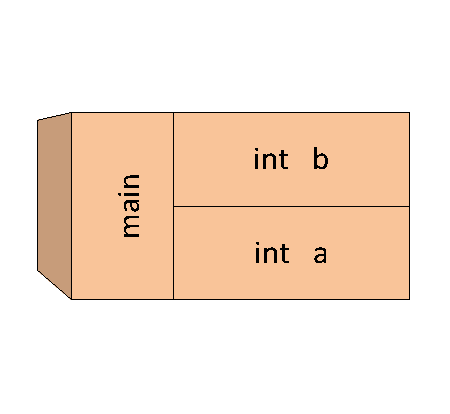
\includegraphics[scale=0.5]{../../Pictures/operator=Int.pdf}
	\end{center}
	\caption{Copie de b en a, cas des entiers.}
	\label{fig:operator=Int}
\end{figure}

Lorsque nous voulons �crire la m�me chose pour des \classname{Complex}, que se passe-t-il ?\\

\begin{DDbox}{\linewidth}
\begin{lstlisting}[caption = affectation d'un Complex par un autre, label=lst:affectation2]
#include "Complex.h"
void main()
{
    Complex c1 = Complex::FromCartesian(1,0);
    Complex c2 = Complex::FromCartesian(0,1);
    c1=c2;
}
\end{lstlisting}\end{DDbox}

Dans le listing \ref{lst:affectation2}, \varname{c1} et \varname{c2} sont deux instances de type Complex diff�rentes, mais dont les champs \varname{\_real} et \varname{\_im} ont m�mes valeurs, \textit{i.e.} \varname{c1.\_real = c2.\_real} et \varname{c1.\_im = c2.\_im} apr�s ex�cution de l'op�rateur \textbf{=}. Cet �tat est �galement d�crit par le graphique \ref{fig:operator=Complex}. Comme pour le cas des entiers, il est tr�s important de noter et de retenir\footnote{Car c'est un comportement tr�s diff�rent de celui de langages comme le C\# ou le Java par exemple.} que si nous �crivons � la suite de l'affectation \varname{c1=c2;} l'instruction : \varname{c1 = Complex::FromCartesian(1,1)}, la valeur de \varname{c2} reste inchang�e.\\

\begin{figure}[]
	\begin{center}
		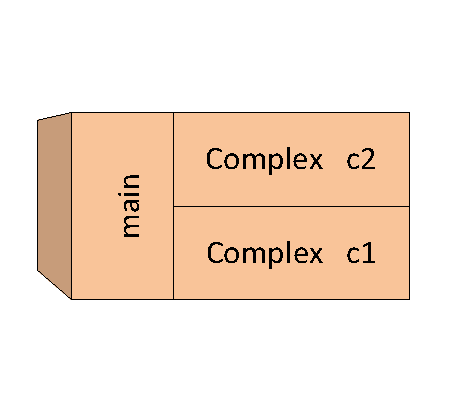
\includegraphics[scale=0.5]{../../Pictures/operator=Complex.pdf}
	\end{center}
	\caption{Copie de b en a, cas des Complexs.}
	\label{fig:operator=Complex}
\end{figure}

Comment le langage r�alise-t-il donc l'affectation (op�rateur \varname{=}) d'une instance de type non primitif en une autre ? Par d�faut, son comportement est tr�s exactement le m�me que le constructeur-copie par d�faut : l'environnement va copier octet par octet tous les champs de l'instance source dans l'instance cible.\\

En r�gle g�n�rale, c'est un comportement raisonnable, et nous pouvons dans la plupart des cas laisser cette impl�mentation par d�faut de l'op�rateur \varname{=}. Cependant, nous verrons que lorsque l'un des champs � recopier est un pointeur, l'impl�mentation par d�faut de l'op�rateur \textbf{=} peut se r�v�ler tr�s dangereuse, et nous voudrons dans ces cas-l� la red�finir nous-m�me explicitement. Afin de comprendre comment la red�finir, nous donnons dans le listing \ref{lst:affectation3}, � titre d'exemple, une red�finition explicite de l'op�rateur \textbf{=} qui se contente de mimer fid�lement l'impl�mentation implicite par d�faut, c'est � dire qui recopie les champs valeur par valeur.\\

\begin{DDbox}{\linewidth}
\begin{lstlisting}[caption = premi�re surcharge de l'op�rateur d'affectation, label=lst:affectation3]
void Complex::operator=(const Complex& source)
{
	_real = source._real;
	_im = source._im;
}
\end{lstlisting}\end{DDbox}

Traditionnellement, et pour des raisons que nous ne d�taillons pas ici\footnote{penser qu'on veut pouvoir �crire \textbf{c1=c2=c3;}}, cet op�rateur doit en r�alit� retourner la nouvelle valeur de l'instance modifi�e. Pour faire cel�, l'instance "appelante" doit donc se retourner elle-m�me. Cette op�ration est possible via l'utilisation du mot clef \classname{this}, qui, appel� dans une m�thode de classe, retourne un pointeur sur l'objet qui appelle la m�thode. Nous pouvons donc dans une m�thode r�cup�rer l'objet "appelant" par "\textbf{*this}", comme dans le listing \ref{lst:affectation4}.\\

\begin{DDbox}{\linewidth}
\begin{lstlisting}[caption = surcharge canonique de l'op�rateur d'affectation, label=lst:affectation4]
Complex& Complex::operator=(const Complex& source)
{
	_real = source._real;
	_im = source._im;
    return *this;
}
\end{lstlisting}\end{DDbox}

\section{Op\'erateurs internes, op\'erateurs externes}
\label{section:InternAndExternOperators}

Un op�rateur est dit membre s'il est d�fini au sein d'une classe : c'est le cas par exemple de l'op�rateur \varname{+=} dans le listing \ref{lst:ComplexOperators} ou de l'op�rateur \varname{=} dans le listing \ref{lst:affectation4}. Dans le cas contraire, il est dit non-membre : c'est par exemple le cas de l'op�rateur \varname{+} dans le listing \ref{lst:ComplexOperators}.\\

Certains op�rateurs doivent n�cessairement �tre impl�ment�s comme des op�rateurs membres. C'est le cas par exemple des op�rateurs \varname{=} (op�rateur d'\textit{assignment} ou d'affectation), de l'op�rateur \varname{[]} (op�rateur crochet ou \textit{array subscription}), de l'op�rateur \varname{->} (op�rateur d'acc�s), ou encore de l'op�rateur \varname{()} (op�rateur \textit{function call}). C'est une contrainte du langage.\\

A l'inverse, certains op�rateurs doivent n�cessairement �tre impl�ment�s comme des op�rateurs non membres. Par exemple, lorsque nous voulons impl�menter des op�rateurs binaires dont l'op�rande de gauche est une classe dont nous ne poss�dons pas le code source : ainsi, si nous voulons donner du sens � \varname{cout << a} o� \varname{a} est une instance de type \classname{A}, nous ne pouvons modifier le code de la classe \classname{std::ostream} dont \varname{cout} est une instance car ce code n'est pas disponible, et nous ne pouvons donc pas impl�menter l'op�rateur
\functionname{<<} comme un op�rateur membre de la classe \classname{std::ostream}.\\

En ce qui concerne les op�rateurs qui ne sont pas sujets aux contraintes sus-nomm�es, ils peuvent �tre d�finis ou bien comme des op�rateurs membres, ou bien comme des op�rateurs non-membres. Pour ces op�rateurs, le meilleur design est sujet � d�bat, mais voici quelques recommendations qui peuvent vous aider � choisir entre les deux designs.\\

\begin{enumerate}
\item Pr�f�rer l'impl�mentation comme op�rateur membre pour les op�rateurs unaires (i.e. ceux qui ne prennent qu'un argument)
\item Si un op�rateur traite ses deux op�randes de mani�re �quivalente, pr�f�rez l'impl�mentation comme op�rateur non-membre
\item Si un op�rateur ne traite pas ses deux op�ratendes de mani�re �quivalente (bien souvent dans ce cas, il modifie en profondeur l'op�rande de gauche) et si il n�cessite un acc�s aux propri�t�s priv�es de ce membre, pr�f�rez l'impl�mentation comme op�rateur membre.\\  
\end{enumerate}
\begin{recapitulatif}
\item Il est possible de surcharger les op\'erateurs classiques, afin de permettre une manipulation plus ais\'ee \`a l'utilisateur de la classe.
\item Un op\'erateur est soit externe, soit interne.
\item Il faut surcharger les op\'erateurs avec parcimonie.
\end{recapitulatif} 
\begin{savequote}
Object-oriented programming is an exceptionally bad idea which could only have originated in California.
\qauthor{propos pr�t� faussement � Edsger Dijkstra, r�el auteur inconnu}
\end{savequote}

\chapter{Les templates}

Les templates sont un m\'ecanisme puissant de factorisation de code, qui permettent d'\'ecrire du code g\'en\'erique s'appliquant \`a des donn\'ees,
ind\'ependamment de leur type. Plus pr\'ecis\'ement, ils permettent de produire en un seul fichier une famille de fonctions ou une famille de
classes indic\'ees par un type abstrait ou par un autre param\`etre comme un entier.\\

\section{Templating par un type, l'exemple des fonctions}

Les templates sont issus originellement d'un souci de simplification de code par la factorisation, afin d'\'eviter les redondances. Prenons
l'exemple d'une fonction Max qui prenne en argument un tableau de double et la taille de ce tableau :\\

\begin{DDbox}{\linewidth}
\begin{lstlisting}
double Max(double array[], int length)
{
    double vmax = array[0];
    for (int i = 1; i < length; i++)
        if (array[i] > vmax)
            vmax = array[i];
    return vmax;
}
\end{lstlisting}
\end{DDbox}

Si nous voulions d\'efinir la m\^eme fonction sur un tableau d'entiers, nous devrions alors produire le code suivant : \\

\begin{DDbox}{\linewidth}
\begin{lstlisting}
int Max(int array[], int length)
{
    int vmax = array[0];
    for (int i = 1; i < length; i++)
        if (array[i] > vmax)
            vmax = array[i];
    return vmax;
}
\end{lstlisting}
\end{DDbox}

De la m\^eme mani\`ere, nous pourrions d\'efinir la fonction Max sur un tableau de float, de ushort, de uint, de long, etc... Dans le cadre
d'exemples plus complexes, le d\'edoublement du code pour chaque type est tr\`es p\'enalisant : tout d'abord, il nuit \`a la clart\'e du code pour
le lecteur, mais il entraine aussi un risque important de divergence des diff\'erentes versions du code. En effet, si la s\'emantique de la fonction
Max est incorrecte, elle le sera \`a la fois pour la version du code manipulant des entiers comme pour celle manipulant des doubles. Si un
d\'eveloppeur est amen\'e \`a am\'eliorer ou d\'ebugger une version de cette fonction, il court le risque d'oublier que d'autres versions de cette
fonction demandent probablement les m\^emes modifications.\\

Nous le concevons donc, \textbf{la redondance du code est \`a proscrire}\footnote{La r\`egle 1 du d\'eveloppement pourrait \^etre : "ne faites pas
de copier/coller de code au sein d'un projet."}. Comment dans ces conditions cr\'eer une seule fonction Max qui permette de d\'efinir cette fonction
pour des entiers, mais aussi pour des double, des uint, etc... ? Le C++ propose un m\'ecanisme pour d\'efinir en une fois le code devant
s'appliquer, quel que soit le type des arguments. Observons la syntaxe suivante : \\

\begin{DDbox}{\linewidth}
\begin{lstlisting}
template<typename T>
T Max(T array[], int length)
{
    T vmax = array[0];
    for (int i = 1; i < length; i++)
        if (array[i] > vmax)
            vmax = array[i];
    return vmax;
}
\end{lstlisting}
\end{DDbox}

Dans cet exemple, la fonction Max devient param\'etr\'ee par un type abstrait T. Celui-ci est utilis\'e dans notre exemple \`a la fois pour
d\'efinir le type du premier argument de la fonction, mais \'egalement pour d\'efinir son type de retour. Le pr\'efixe template<typename T> indique
au compilateur que le code qui suit sera param\'etr\'e par un type T. De mani\`ere \'equivalente, le mot clef \textit{typename} peut \^etre
remplac\'e par \textit{class}.\\

Lorsque dans notre code, nous voulons utiliser notre fonction Max, nous pouvons le faire de la sorte :\\

\begin{DDbox}{\linewidth}
\begin{lstlisting}
int values[]={ 16, 8, 3, 2, 11 };

cout << Max<int>(values, 5);
\end{lstlisting}
\end{DDbox}

Lorsque le compilateur va lire l'appel \`a Max(values, 5), il va d\'etecter qu'il s'agit d'utiliser la fonction templat\'ee Max dans le cas o\`u T =
int. Le compilateur va alors g\'en\'erer le code correspondant et l'inclure dans la compilation. Bien \'evidemment, le compilateur ne g\'en\`erera
la fonction Max que pour les types T pour lesquels il est fait appel quelque part \`a la fonction Max utilis\'ee pour le type T : si nulle part dans
notre code nous ne cherchons \`a d\'eterminer le max d'un tableau de double, le code sp\'ecifique pour la fonction Max en le type double ne sera pas
g\'en\'er\'e.\\

Le fait d'utiliser une fonction templat\'ee en un type sp\'ecifique est appel\'e \textit{sp\'ecialisation}. Pouvons-nous sp\'ecialiser la fonction
Max en n'importe quel type ? L'approche du C++ sur la question est une approche optimiste (\`a la diff\'erence du C\# par exemple) : par d\'efaut,
tout type est accept\'e. C'est uniquement \`a la compilation que le compilateur va tenter de g\'en\'erer le code n\'ecessaire pour chacun des types
en lesquels la fonction templat\'ee a \'et\'e sp\'ecialis\'ee. Si notre fonction est sp\'ecialis\'ee en un type T1 pour lequel l'op\'erateur < n'est
pas d\'efini, alors le compilateur \'echouera dans la g\'en\'eration du code sp\'ecialis\'e.\\

\subsection{Templates et macro}

Si nous reprenons la fonction templat\'ee pr\'ec\'edente appliqu\'ee \`a deux valeurs plut\^ot qu'\`a un tableau, nous pouvons produire le code
suivant :\\

\begin{DDbox}{\linewidth}
\begin{lstlisting}
template<typename T>
const T & Max( const T & a, const T & b )
{
    return a > b ? a : b;
}
\end{lstlisting}
\end{DDbox}

Cet exemple ressemble beaucoup avec la macro correspondante, comme d\'etaill\'ee dans le chapitre sur la compilation :\\

\begin{DDbox}{\linewidth}
\begin{lstlisting}
#define MAX(a, b) (((a) > (b)) ? (a) : (b))
\end{lstlisting}
\end{DDbox}

En effet, dans chaque cas, nous avons une impl\'ementation de la fonction max qui peut s'adapter \`a tous types d'objets. Le templating est la
mani\`ere propre d'\'ecrire des macros. L\`a o\`u la macro est une simple substitution syntaxique, avec toutes les erreurs qui en d\'ecoulent
(\ref{sec:macros}), le templating g\'en\`ere de r\'eelles fonctions et permet donc d'obtenir de mani\`ere fiable le r\'esultat.\\

Dans la comparaison qui vient d'\^etre faite, il faut noter cependant qu'un avantage majeur de la macro par rapport \`a son homologue templat\'ee
est l'absence d'appel de fonction : puisque la macro ne cr\'ee pas de v\'eritable fonction, il n'y a pas d'appel de fonction et donc pas de co\^ut
d'appel de fonction. Il est possible d'\'eviter ce co\^ut \'egalement dans le cas d'une fonction templat\'ee, en l'inlinant :\\

\begin{DDbox}{\linewidth}
\begin{lstlisting}
template<typename T>
inline const T & Max( const T & a, const T & b )
{
    return a > b ? a : b;
}
\end{lstlisting}
\end{DDbox}

\subsection{Fonctions membres templat\'ees}

Il est \'egalement possible de cr\'eer une fonction templat\'ee au sein d'une classe non templat\'ee. L'exemple suivant d\'ecrit une classe
disposant d'une fonction membre templat\'ee permettant d'afficher diff\'erente objets.\\

\begin{DDbox}{\linewidth}
\begin{lstlisting}
class SomeClass
{
    public SomeClass();
    public ~SomeClass();

    template<typename T>
    static void Display( const T & t )
    {
        cout << t;
    }
}

int main()
{
    SomeClass.Display<int>(2);
    SomeClass.Display<string>("Hello World");
    SomeClass.Display<double>(3.14);
}
\end{lstlisting}
\end{DDbox}

\subsection{Inf\'erence automatique de type de sp\'ecialisation}

Lorsque le compilateur est capable d'inf\'erer le type en lequel est sp\'ecialis\'ee une fonction templat\'ee, il est superflu de sp\'ecifier
explicitement en quel type la fonction est sp\'ecialis\'ee. Dans le cas du code pr\'ec\'edent par exemple, nous pourrions \'ecrire :\\

\begin{DDbox}{\linewidth}
\begin{lstlisting}
int main()
{
    SomeClass.Display(2);
    SomeClass.Display("Hello World");
    SomeClass.Display(3.14);
}
\end{lstlisting}
\end{DDbox}

Il est cependant des cas o\`u une telle inf\'erence n'est pas possible, notamment dans le cas d'ambigu\"it\'e que le compilateur ne peut pas lever
lui-m\^eme. Ainsi, la fonction suivante doit \^etre sp\'ecifi\'ee explicitement :\\

\begin{DDbox}{\linewidth}
\begin{lstlisting}
template <typename T>
T Sum( T s1, T s2 )
{
    return s1 + s2;
}

int main()
{
    int s2 = 1;
    double s1 = 3.2;

    Sum( s1, s2 ); // Erreur : paramètre ambigü
    Sum<double>( s1, s2 ); // OK
}
\end{lstlisting}
\end{DDbox}

\subsection{Multi-templating}

Il est possible de param\'etrer une fonction par plusieurs arguments; en voici un exemple :\\

\begin{DDbox}{\linewidth}
\begin{lstlisting}
template<typename T, typename U>
public T Add (const T& t, const U& u)
{
    return t+u;
}
\end{lstlisting}
\end{DDbox}

\section{Templating par un type, le cas des classes}

De la m�me mani�re que nous avons d�fini le param�trage d'une fonction par un type g�n�rique T, nous pouvons param�trer une classe par un type g�n�rique.  Le templating par des classes est principalement utilis� pour construire des "containers", c'est � dire des classes dont la fonction est de contenir un ensemble d'�l�ments d'un m�me type. Un exemple �clairant sera donn� dans la section \ref{subsection:VectorCode}.

\section{Templates et compilation}

Un voile pudique est bien souvent jet� par les manuels d'introduction au C++ sur la compilation des templates. Ceux-ci r�pondant � des contraintes bien particuli�res (puisqu'il ne s'agit pas de code mais de "m�ta-code"), il n'est pas possible par d�faut de d�clarer une fonction template dans un fichier .h puis de la d�finir dans un fichier .cpp. Par d�faut, il vous faudra donc m�langer d�claration et d�finition dans un m�me fichier .h sous peine de vous exposer � des erreurs � l'�dition des liens. Comme il est expliqu� dans l'article d'Aur�lien Regat-Barrel sur le site cpp.developpez.com, il existe n�anmoins une astuce permettant de contourner le probl�me.\\

Cette astuce consiste � stocker la d�claration de votre classe templat�e dans un fichier .h, de stocker votre d�finition dans un fichier texte (avec une extension diff�rente de .cpp, comme .tpp par exemple), et d'inclure gr�ce � l'instruction \#include le fichier .tpp � la fin du fichier header. Ainsi, nous obtenons par exemple quelquechose de la forme : \\

\begin{DDbox}{\linewidth}
\begin{lstlisting}
// exemple.h

#ifndef EXEMPLE_H
#define EXEMPLE_H

template <typename T>
class Exemple
{
public:
    Exemple();
};

#include "exemple.tpp" // voici l'astuce
#endif

// exemple.tpp

template <typename T>
Exemple<T>::Exemple()
{
}

\end{lstlisting}
\end{DDbox}

\section{Templates et sp�cialisation}

Il existe certains cas o� nous voudrions faire des exceptions � la g�n�ricit�, c'est � dire que pour certains types bien particuliers, une fonction templat�e ait un comportement particulier, qui diff�re du comportement g�n�ral d�j� d�fini. Prenons le cas de l'exponentiation de 2. Si $y$ est un r�el (double ou float), le calcul de $2^{y}$ demande de r��crire la formule en $e^{y.ln(2)}$ afin de l'�valuer. Nous pourrions donc �crire :\\

\begin{DDbox}{\linewidth}
\begin{lstlisting}

template<typename T>
double TwoPow(T y)
{
    return exp(y*ln(2);
}
\end{lstlisting}
\end{DDbox}

Cette fonction fonctionnerait �galement si elle �tait sp�cifi�e en deux entiers. Cependant, dans le cas o� y est entier, il n'est pas n�cessaire de passer par cette formule, il suffit alors de multiplier 2 par lui m�me y fois. Bien que la formule pr�c�dente soit exacte dans le cas o� y est entier, elle entrainerait donc des calculs ind�ment longs. Pour am�liorer cette situation, nous voudrions dire au compilateur : compile la fonction pr�c�dente pour tous les types n�cessaires, SAUF dans le cas o� y est entier, auquel cas contente toi de calculer directement la valeur de l'exponentiation. En C++, il est possible de pr�ciser/red�finir une sp�cialisation sp�cifique.\\

\begin{DDbox}{\linewidth}
\begin{lstlisting}

// Sp�cialisation pour les int
template <>
double TwoPow<int>( int i )
{
    double q= (i >= 0) ? 2 : 0.5;
    int iAbs = abs(i);
    double r=1;

    for (int j = 0 ; j < iAbs;j++)
        r*=q;

    return r;
}

\end{lstlisting}
\end{DDbox}

\subsection{Sp�cialisation partielle}

Les templates peuvent �tre partiellement sp�cialis�s, et la classe obtenue est alors encore un template. Cette sp�cialisation partielle intervient principalement dans le cas dans le cas d'un template param�tr� par plusieurs types, pour lesquels seuls certains de ces types sont sp�cialis�s, le r�sultat �tant un template param�tr� dans les types restants. Exemple :\\

\begin{DDbox}{\linewidth}
\begin{lstlisting}
template<typename T, typename U>
public double Pow(T x, U y)
{
    return exp(y*ln(x));
}

template<typename T>
public double Pow<T,int>(T x, int y)
{
    double q= (y >= 0) ? x : ((double)1)/x; //do not forget the explicit cast into double !
    int yAbs = abs(y);
    double r=1;

    for (int j = 0 ; j < yAbs;j++)
        r*=q;

    return r;
}
\end{lstlisting}
\end{DDbox}

\section{Templating par des entiers}

Il est �galement possible de param�trer une fonction par autre chose qu'un type. Notamment, il est possible de param�trer une fonction par un entier. Ces m�canismes ne seront pas d�taill�s cette ann�e, mais ils sont massivement utilis�s dans de nombreuses librairies professionnelles, car ils permettent des optimisations tr�s fines, notamment via le Template Meta-Programming. Les bonnes librairies de calcul scientifique en C++ par exemple reposent toutes massivement sur ce genre d'optimisation. Nous renvoyons le lecteur int�ress� par exemple � \cite{Alexandrescu}. 
\begin{savequote}[130mm]
In the fairy tales about heroes defeating evil villains there's always a dark
forest of some kind. It could be a cave, a forest, another planet, just some
place that everyone knows the hero shouldn't go. Of course, shortly after the
villain is introduced you find out, yes, the hero has to go to that stupid
forest to kill the bad guy. It seems the hero just keeps getting into
situations that require him to risk his life in this evil forest.\\

You rarely read fairy tales about the heroes who are smart enough to just avoid the whole situation entirely. You never hear a hero say, "Wait a
minute, if I leave to make my fortunes on the high seas leaving Buttercup behind I could die and then she'd have to marry some ugly prince named
Humperdink. Humperdink! I think I'll stay here and start a Farm Boy for Rent business." If he did that there'd be no fire swamp, dying, reanimation,
sword fights, giants, or any kind of story really. Because of this, the forest in these stories seems to exist like a black hole that drags the hero
in no matter what they do.\\

In object-oriented programming, Inheritance is the evil forest. Experienced programmers know to avoid this evil because they know that deep inside
the Dark Forest Inheritance is the Evil Queen Multiple Inheritance. She likes to eat software and programmers with her massive complexity teeth,
chewing on the flesh of the fallen. But the forest is so powerful and so tempting that nearly every programmer has to go into it, and try to make it
out alive with the Evil Queen's head before they can call themselves real programmers. You just can't resist the Inheritance Forest's pull, so you
go in. After the adventure you learn to just stay out of that stupid forest and bring an army if you are ever forced to go in again.\\
\qauthor{http://learnpythonthehardway.org/book/ex44.html}
\end{savequote}



\chapter{H�ritage et Composition}
\label{chapter:inheritance}

\section{H�ritage simple}

L'h�ritage est un des aspects fondamentaux de la programmation orient�e-objet. Il permet de transmettre (\textit{de faire h�riter})les propri�t�s d'une classe (m�thodes et champs) � une autre classe, participant ainsi � la structuration des projets autour des classes.

\subsection{Motivation}

Par les vicissitudes d'une faille spatio-temporelle, vous vous retrouvez t�l�port� dans la peau d'un d�veloppeur pour une soci�t� de location de v�los et de voitures. Votre premier jet met en place les classes Bike et Car d�crites dans les listings \ref{lst:Car1.h} et \ref{lst:Bike1.h}.\\

Pour ne pas perturber l'utilisateur des classes, ce sont les m�mes noms de variable qui sont utilis�s dans les deux cas.\\

Nous faisons les remarques suivantes :
\begin{itemize}

	\item Les v\'elos et les voitures sont tous deux des v\'ehicules et
		partagent de nombreuses caract\'eristiques (prix, couleur,
		\'etat), mais ont cependant des diff\'erences.

	\item Si nous voulons ajouter un autre type de v�hicule (des motos,
		par exemple), il va nous falloir recr�er une nouvelle classe presque
		identique aux pr\'ec\'edentes.\\
\end{itemize}

\includecode{Car1.h}
\includecode{Bike1.h}


L'impression g�n�rale qui se d�gage du code est une certaine lourdeur, li�e aux redondances observ�es entre les classes Bike et Car. Dans la suite, nous cherchons � isoler ces redondances pour les factoriser et les �crire une seule fois.

\subsection{H�ritage simple et public}

En informatique, cette factorisation est appel�e \textit{h�ritage}, et consiste � isoler le code commun pour cr�er une classe avec les propri�t�s communes, que nous appellerons \textit{classe m�re}. Les \textit{classes filles} ou \textit{classes d�riv�es}, dans notre exemple Car et Bike, vont h�riter de cette classe m�re et en poss�deront toutes les propri�t�s.\\

\includecode{vehicule2.h}
\includecode{voiture2.h}
\includecode{velo2.h}

D'un point de vue syntaxique, la d\'eclaration d'une classe d\'eriv\'ee est donc
tr\`es simple. Il y a trois possibilit\'es :\\

\begin{DDbox}{\linewidth}
\begin{lstlisting}
/*premiere possibilite*/
class Fille : public class Mere
{
    /*nouveaux membres*/
};
/*seconde possibilite*/
class Fille : protected class Mere
{
    /*nouveaux membres*/
};
/*troisieme possibilite*/
class Fille : private class Mere
{
    /*nouveaux membres*/
};

\end{lstlisting}
\end{DDbox}

Le lecteur attentif aura remarqu\'e l'emploi des mots public, protected, ou
private. Nous n'utilisons que la forme
\texttt{public} pour le moment et parlons alors d'h�ritage publique. Les autres types d'h�ritage sont bri�vement abord�s dans la section suivante.\\

La notion d'h�ritage pr�sente les int�r�ts suivants :\\

\begin{enumerate}
\item Le code factoris� est plus court : les propri�t�s communes ne sont pas �crites plusieurs fois.
\item le code factoris� est plus lisible : la structure d'h�ritage participe � une meilleur compr�hension du code. En particulier, elle indique les structures de d�pendances ou de similarit�s entre classes.
\item Le code factoris� est plus extensible : il suffit d'ajouter ou de modifier un champ ou une m�thode dans la classe m�re pour en faire b�n�ficier toutes les classes filles.
\item Le code factoris� est plus maintenable : lorsque nous voulons modifier le code d'une m�thode non factoris�e mais dupliqu�e au sein de plusieurs classes, il faut la modifier dans chacune des classes de la m�me mani�re exactement et dans toutes ces classes, faute de quoi les m�thodes qui �taient les m�mes commencent � diff�rer. Lorsque le code est factoris�, il suffit de le modifier une seule fois.
\end{enumerate}

Nous pouvons appeler les m\'ethodes de la classe m�re
\texttt{Vehicule} comme \varname{double GetPrice(void)} depuis un objet \texttt{Bike} ou \texttt{Car} comme si ces m�thodes �taient impl�ment�es dans les classes filles. Par exemple, le code-ci dessous fonctionnera correctement:\\

\begin{DDbox}{\linewidth}
\begin{lstlisting}
Bike b;

cout << b.GetPrice();
\end{lstlisting}
\end{DDbox}

\subsection{Le mot clef "protected"}

Lors de notre introduction \`a l'encapsulation, nous avions vu deux mots
cl\'es : \keyword{private} et \keyword{public}. \keyword{private} servait \`a
interdire au reste du monde d'acc\'eder \`a certains membres, et
\keyword{public} servait \`a autoriser le reste du monde \`a acc\'eder \`a
certains membres.\\

Que se passe-t-il si nous voulons dans une m�thode fille acc�der � un champ \keyword{private} de la classe m�re ? Supposons par exemple que nous ajoutions une m�thode \varname{void DisplayCost()} dans la classe Car, d�finie de la mani�re suivante : \\

\begin{DDbox}{\linewidth}
\begin{lstlisting}
void Car::DisplayCost(void)
{
    cout << "Cost of this car is : " << _price << " euros.\n"
}
\end{lstlisting}
\end{DDbox}

Si nous compilons le code pr\'esent\'e, le compilateur va nous donner une erreur :\\

\texttt{'\_price' : cannot access private member declared in class 'Vehicule'}\\

Que signifie cette erreur? Son origine est l'inaccessibilit�/l'invisibilit� de la variable \varname{\_price} dans les m�thodes de la classe \varname{Car}. Nous avons en effet implicitement suppos\'e que nous avions acc\`es dans nos classes d\'eriv\'ees aux membres priv\'es de la classe m\`ere. Ce n'est pas le cas.\\

Dans le cadre de l'h\'eritage (publique) que nous traitons depuis le d�but, nous avons donc le comportement suivant :

\begin{itemize}
	\item Les membres \keyword{private} de la classe m\`ere ne sont \emph{pas} accessibles \`a la classe d\'eriv\'ee.
	\item Les membres \keyword{public} de la classe m\`ere sont accessibles \`a la classe d\'eriv\'ee.\\	
\end{itemize}

Nous ajoutons maintenant un niveau interm�diaire dans lequel les champs de la classe m�re sont accessibles � la fois dans les m�thodes de la classe m�re et des classes filles, mais qui ne sont pas accessibles de l'ext�rieur de ces classes (comme par exemple dans le main). Le mot clef qui permet de d�finir ce niveau interm�diaire est le mot \keyword{protected}.\\

L'ensemble de ces r\`egles d'h\'eritage est r\'esum\'e dans le tableau \ref{tab:encapsulationvisibilite}.\\

\begin{table}
	\centering
	\begin{tabular}{l|l|l|l}
	Acc\`es	& public & protected & private\\
	\hline
	Membres de la classe & Oui & Oui & Oui \\
	\hline
	Membres des classes d\'eriv\'ees & Oui & Oui & Non\\
	\hline
	Reste du monde & Oui & Non & Non\\
	\hline
	\end{tabular}
	\caption{Encapsulation : diff\'erents degr\'es de visibilit\'e (cas de l'h�ritage publique)}
	\label{tab:encapsulationvisibilite}
\end{table}

Pour que nos classes d\'eriv\'ees aient acc\`es au membre \varname{\_price}, nous avons donc deux possibilit\'es :

\begin{itemize}
	\item  Utiliser l'accesseur \functionname{GetPrice};
	\item  Mettre \varname{\_price} en \keyword{protected}.
\end{itemize}

Nous allons retenir la seconde solution, et notre classe \classname{Vehicule} s'\'ecrira alors:\\

\includecode{vehicule3.h}

\subsection{Constructions et destructions d'objets filles}

Dotons-nous tout d'abord d'une classe m�re avec deux constructeurs distincts, pour lesquels une sortie console est affich�e � chaque appel, afin de savoir quand et quel constructeur a �t� appel�.\\

\includecode{Mother.h}
\includecode{Mother.cpp}

Nous cr�ons alors une classe Child qui d�rive publiquement de Mother.\\

\includecode{Child.h}
\includecode{Child.cpp}

Lorsque nous voulons construire un objet fille dans notre main, via par exemple le code suivant : \\

\begin{DDbox}{\linewidth}
\begin{lstlisting}
#include "Child.h"

void f()
{
    Child c;
}

void main()
{
    f();
}

\end{lstlisting}
\end{DDbox}

Nous pouvons lire apr�s la fin de la fonction main dans la console les lignes suivantes : \\

\texttt{Default mother constructor called\\}
\texttt{Child empty constructor called\\}
\texttt{Child destructor called\\ }
\texttt{Mother destructor called\\ }

Nous observons ainsi que la construction d'un objet fille appelle implicitement un constructeur m�re avant d'appeler le constructeur de la classe fille. De m�me, � la destruction de notre objet, le destructeur de la classe m�re est appel� apr�s le destructeur de la classe fille.\\

A la construction de notre objet fille, quel est le constructeur m�re appel� ? Si nous ne le sp�cifions pas, c'est le constructeur m�re par d�faut qui est appel�, comme nous le voyons par le message de la console. Il est cependant possible d'expliciter quel constructeur de la classe m�re nous voulons utiliser au d�but de la d�finition de notre constructeur fille. Ainsi, nous pouvons modifier de la sorte le constructeur fille pour que ce soit le constructeur m�re avec 1 argument qui soit appel� :\\

\includecode{Child2.cpp}

\bigskip
\begin{warning}
Si vous ne sp�cifiez pas explicitement le constructeur m�re � appeler lorsque vous construisez une fille, nous avons vu que c'�tait le constructeur m�re par d�faut qui �tait appel�. Dans un tel cas, et si le constructeur m�re par d�faut n'existe pas (par exemple si vous avez d�clar� un seul constructeur dans Mother.h qui prend en argument des param�tres), alors votre IDE �chouera � compiler, vous sp�cifiant un message de la sorte :\\

\texttt{Error C2512: 'Mother' : no default appropriate constructor available in child.cpp (l5)}

\end{warning}

\section{Autres h�ritages}

\subsection{H�ritage protected et private}

Nous avions mentionn\'e dans la section pr�c�dente qu'il \'etait possible de
d\'eclarer une classe d\'eriv\'ee au moyen de trois mots cl\'es diff\'erents :
\keyword{private}, \keyword{protected}, et \keyword{public}. Jusqu'\`a
pr\'esent, nous n'avons employ\'e que le mot cl\'e \keyword{public}. Que
signifie-t-il pr\'ecis\'ement?\\

En r�alit�, chacun des mots clefs (public, private ou protected) agit comme une sorte de filtre sur la visibilit\'e des membres de la classe m\`ere. Pour ce point, la mani�re la plus claire de d�finir ces diff�rents filtres est d'en donner un exemple :\\

\begin{DDbox}{\linewidth}
\begin{lstlisting}
class Mother
{
    public:
        int x;
    protected:
        int y;
    private:
        int z;
};

class Child1 : public Mother
{
    // x is public
    // y is protected
    // z is not accessible from Child1
};

class Child2 : protected Mother
{
    // x is protected
    // y is protected
    // z is not accessible from Child2
};

class Child3 : private Mother
{
    // x is private
    // y is private
    // z is not accessible from Child3
};
\end{lstlisting}
\end{DDbox}

\subsubsection{Quand utiliser de l'h�ritage protected ou private ?}

Il y a encore d�bat aujourd'hui, mais une r�ponse assez commun�ment accept�e est : jamais. L'h�ritage protected ou private sert � pouvoir utiliser quelquechose sans en donner directement acc�s de l'ext�rieur. Il est en cel� tr�s proche de la composition, d�taill�e ci-dessous. Nous recommendons de passer plut�t par de la composition que par un h�ritage protected ou private. Pour trouver des exemples pertinents d'h�ritage private, nous renvoyons le lecteur par exemple � la programmation par "Policies" d'Alexandresc� \cite{Alexandrescu}, mais c'est un exemple qui exc�de largement notre propos.\\

\subsection{H�ritage multiple et virtuel}


Nous avons vu dans la section pr\'ec\'edente que l'h\'eritage permet de
d\'ecrire une relation ``est un'' entre deux objets. Cependant, comment faire
dans le cas o\`u un objet ``est un'' X \emph{et} un Y ? L'h\'eritage multiple
permet de r\'esoudre ce probl\`eme. Avant de poursuivre, il nous semble important de
pr\'eciser que l'h\'eritage multiple est aussi \emph{dangereux\footnote{Il
est consid\'er\'e comme suffisamment dangereux pour \^etre explicitement
interdit dans les langages r�cents comme le JAVA ou le C\#. Le manque d'interface en C++ ne laisse maheureusement parfois pas d'autre choix que d'utiliser un h�ritage multiple. Nous ne saurions trop vous inciter n�anmoins � l'utiliser avec la plus grande circonspection} que toxique}, pour
des raisons qui deviendront claires par la suite mais qui ont d�j� �t� esquiss�es dans la citation de d�but de chapitre.

\subsubsection{Principe}

L'id\'ee est assez naturelle : nous allons faire h\'eriter notre classe
d\'eriv\'ee de \emph{deux} classes m\`eres. D'un point de vue syntaxique, on \'ecrira:

\begin{DDbox}{\linewidth}
\begin{lstlisting}
	class Child :
		public|protected|private class Mother1,
		public|protected|private class Mother2,
		. . .
		public|protected|private class MotherN
	{
	}		
\end{lstlisting}
\end{DDbox}

Par exemple, consid\'erons les classes de v\'ehicules pr\'ec\'edentes, et
ajoutons une nouvelle classe repr\'esentant un avion (ou tout autre objet
volant), qui va \'egalement d\'eriver de \classname{Vehicule}. Celui-ci aura
une nouvelle propri\'et\'e qui sera l'altitude maximum \`a laquelle le v\'ehicule peut voler.

\includecodecaption{avion4.h}{V\'ehicule volant}

Supposons \`a pr\'esent que nous souhaitions manipuler une voiture volante. Une telle voiture est \`a la fois un v\'ehicule volant et une voiture. Nous pouvons donc avoir recours \`a l'h\'eritage multiple et \'ecrire :

\includecode{voiturevolante.h}

Nous pouvons repr\'esenter l'ensemble des relations entre nos classes sur le
diagramme de la figure \ref{fig:heritageVehiculeVolant}.\\

\begin{figure}[]
	\begin{center}
		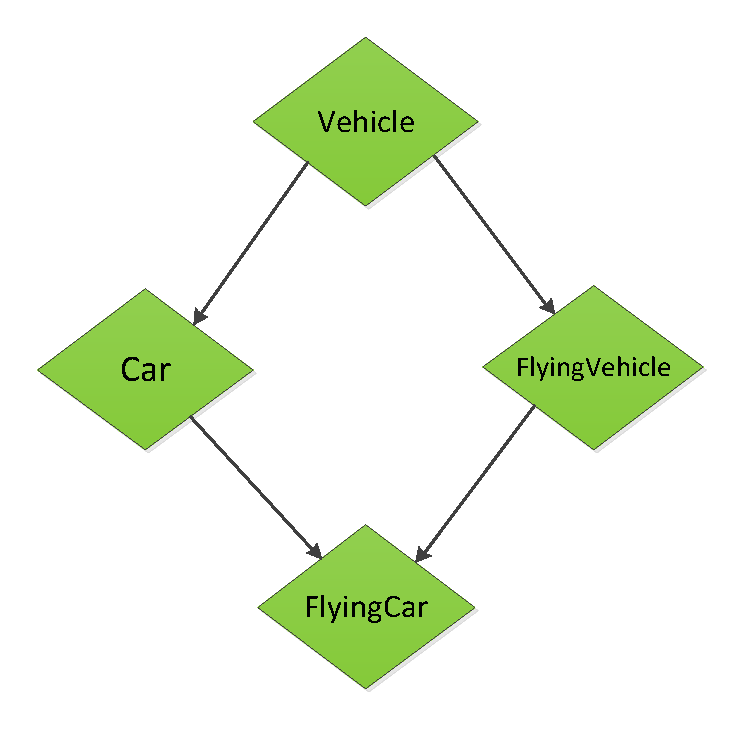
\includegraphics[scale=0.5]{../../Pictures/diamond}
	\end{center}
	\caption{H\'eritage multiple, le diamant}
	\label{fig:heritageVehiculeVolant}
\end{figure}

Comme aurait pu dire Vinz dans La Haine, "Jusqu'ici, tout va bien", et les choses nous paraissent assez naturelles. Cependant, nous pouvons
remarquer que \classname{FlyingCar} d\'erive de \classname{Car}  et
\classname{FlyingVehicle}, qui d\'erivent elles-m\^eme de la m\^eme classe de
base \classname{Vehicle}. Si nous regardons le dessin form\'e par les bo\^ites
d\'ecrivant les objets et les fl\`eches les reliant (figure
\ref{fig:heritageVehiculeVolant}), nous constatons que l'ensemble forme - au moins
approximativement - un losange, qui prend le nom de "Deadly Diamond of Death".\\

C'est l\`a que se trouve la difficult\'e principale de l'h\'eritage multiple,
que nous explicitons \`a pr\'esent.

\subsubsection{Deadly Diamond of Death}

Le probl\`eme est le suivant : le champ \varname{\_color} a
\'et\'e d�clar� dans la classe \classname{Vehicle}, et il est donc h�rit� dans les classes \classname{FlyingCar} et
\classname{Car}. Supposons maintenant que nous ajoutions une m\'ethode \`a
\classname{FlyingCar} qui fasse appel � ce champ :\\

\begin{DDbox}{\linewidth}
\begin{lstlisting}
void VehiculeVolant::DisplayColor()
{
	cout << "The color of our new brand flying car is " << \_color << ".\n";
}
\end{lstlisting}
\end{DDbox}

\`A la compilation, cette m\'ethode va provoquer une erreur. Pourquoi? Le
probl\`eme est que le champ \varname{\_color} qui a \'et\'e
d\'efini dans les classes m\`eres est h\'erit\'e \emph{deux fois} (une par l'h�ritage de \classname{Car} et une par l'h�ritage de \classname{FlyingVehicle}). L'appel
\`a ce champ dans \classname{FlyingCar} est donc ambigu. Le C++ nous fournit une technique permettant de lever cette ambig�it\'e, technique qui porte le nom d'\emph{h\'eritage virtuel}.

\subsubsection{H\'eritage virtuel}

La technique consiste simplement \`a pr\'eciser au compilateur qu'il ne doit
h\'eriter des champs et des m�thodes de la classe \classname{Vehicle} qu'une seule fois,
et non deux. Cela se fait au moyen du mot cl\'e \keyword{virtual} que l'on
\'ecrira devant le nom de la classe dont on h\'erite :\\

\begin{DDbox}{\linewidth}
\begin{lstlisting}
class child : public virtual Mother
{
}
\end{lstlisting}
\end{DDbox}

Les headers de nos classes \classname{FlyingVehicle} et \classname{Car} deviendront donc:\\

\includecodecaption{avion4.h}{vehiculeVolant4.h}
\includecode{voiture5.h}

\section{Composition et Aggr�gation}

\subsection{Composition}

Jusqu'� pr�sent, toutes nos classes poss�daient des champs publics ou priv�s de type primitif (comme des int, des double, des boolean). En r�gle g�n�rale, nous voulons avoir plus d'expressivit� et pouvoir disposer de champs de tout type. Pour faciliter la construction de classes avanc�es � partir de classes plus �l�mentaires, le C++ permet justement de composer les objets, c'est-�-dire de fournir dans une classe des champs du type d'une autre classe. Ainsi, nous pourrons �crire :\\

\begin{DDbox}{\linewidth}
\begin{lstlisting}
class A 
{
    public:
        A();
        ~A();
};

class B
{
    public:
        B(A a);
        ~B();
        
    private:
        A _a;        
};

B::B(A a)
{
    _a = a;
}

\end{lstlisting}
\end{DDbox}

Si l'h�ritage exprime une relation de "Est un" entre la classe m�re et la classe fille, la composition permet ainsi d'exprimer la relation "Poss�de un" entre deux classes.\\

Il est important de noter que l'objet poss�dant (\classname{B} dans notre exemple) "d�tient" les objets poss�d�s. Lorsque l'objet poss�dant (souvent d�sign� sous le terme d'objet composite) est construit, le param�tre a est pass� par valeur, le constructeur-copie est appel�, et \classname{B} d�tient alors une copie de \varname{a}, not�e \varname{\_a}. De la m�me mani�re, lorsque l'objet poss�dant (\classname{B}) est d�truit, les objets poss�d�s (\varname{\_a}) sont d�truits simultan�ment.

\subsection{Aggr�gation}

Un cas un peu plus subtil appara�t quand nous ne voulons pas de la notion de possession d�crite dans le cas de la composition. Nous pouvons alors dans notre classe \classname{B} poss�der un pointeur sur \classname{A}, plut�t qu'une instance de la classe \classname{A}.\\

\begin{DDbox}{\linewidth}
\begin{lstlisting}
class A
{
    public:
        A();
        ~A();
};

class B
{
    public:
        B(A* pa);
        ~B();

    private:
        A* _pa;
};

B::B(A* pa)
{
    _pa = pa;
}

\end{lstlisting}
\end{DDbox}

Dans ce cas, l'instance \varname{a} a une existence ind�pendamment de la construction, de l'existence, ou de la destruction des instances de classe \classname{B}.\\

En r�gle g�n�rale, l'aggr�gation est pr�f�r�e � la composition pour �viter de copier des objets, ou lorsqu'il est manifeste que les deux types d'objets doivent avoir des existences qui ne sont pas subordonn�es l'une � l'autre.\\

Il existe un cas o� l'aggr�gation est indispensable, c'est lorsqu'une classe \classname{A} doit poss�der des champs de type A. Dans ce contexte, une composition m�nerait par r�cursion � une cr�ation infinie d'instances de type \classname{A} (en construisant la premi�re instance, il faudrait construire la deuxi�me instance qui est le champ de la premi�re, pour construire la deuxi�me instance il faudrait construire la troisi�me qui est le champ de la deuxi�me, etc.). Nous obtenons alors le code suivant :\\

\begin{DDbox}{\linewidth}
\begin{lstlisting}
class A
{
    public:
        A(A* pa);
        ~A();
        
    private:
        A* _inner;
};

A::A(A* pa)
{
    _inner = pa;
}

\end{lstlisting}
\end{DDbox}

Donnons deux exemples plus concrets de cas d'utilisation.\\ 

Le premier exemple est une classe \classname{User} correspondant aux informations stock�es par utilisateur dans un r�seau social. Une des raisons principales des r�seaux sociaux �tant de pouvoir d�clarer au monde que nous sommes pass�s d'un statut de "single" � "it's complicated with \varname{Trucmuche}", nous voulons pouvoir stocker dans chaque instance un pointeur vers \varname{Trucmuche}. Le code \ref{} en donne un aper�u.\\

\begin{DDbox}{\linewidth}
\begin{lstlisting}
class FbUser
{
    public:
        FbUser(string name, int id, string status, FbUser* pa);
        ~FbUser();

    private:
        FbUser* _mate;
        string _name;
        string _status;
        int _id;
};

\end{lstlisting}
\end{DDbox}

Le second exemple est la construction r�cursive d'un arbre binaire (sch�matis� dans le graphique \ref{fig:BinaryTree}). Dans ce premier exemple, chaque noeud de type \classname{Node} d�tient deux pointeurs vers ses deux noeuds fils (\varname{\_left} et \varname{\_right}). Dans le cas d'un noeud sans fils (i.e. une feuille), les pointeurs valent \varname{NULL}. Dans cet architecture, un arbre est donc une structure poss�dant un pointeur sur le premier noeud (la racine).\\

\begin{figure}[]
	\begin{center}
		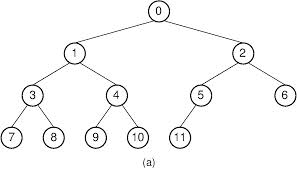
\includegraphics[scale=0.8]{../../Pictures/BinaryTree}
	\end{center}
	\caption{Exemple d'arbre binaire}
	\label{fig:BinaryTree}
\end{figure}

\begin{DDbox}{\linewidth}
\begin{lstlisting}
class Node
{
    public:
        Node(Node* left, Node* right);
        ~Node();

    private:
        Node* _left;
        Node* _right;
};

\end{lstlisting}
\end{DDbox}

Par abus de langage, les concepts de Composition et d'Aggr�gation sont souvent confondus sous le terme Composition.\\

\subsection{D�pendances cycliques et D�clarations Forward}

Il peut arriver qu'une classe \classname{A} contienne un champ (ou un argument d'une m�thode) de type classe \classname{B} et que la classe \classname{B} contienne elle aussi un champ (ou un argument d'une m�thode) de type classe \classname{A}\footnote{Nous pouvons complexifier � volont� ce design, par exemple avec \classname{A} qui d�pend de \classname{B}, \classname{B} qui d�pend de \classname{C} et \classname{C} qui d�pend de \classname{A}}. Nous avons alors une d�pendance cyclique. Si nous incluons A.h dans B.h et B.h dans A.h, nous avons un probl�me d'inclusion cyclique et la compilation �chouera.\\

La solution � ce probl�me est d'utiliser des d�clarations forward. Au lieu d'inclure le header d�clarant \classname{A} dans B.h ou dans B.cpp, nous  d�clarons seulement le type \classname{A} pour indiquer au compilateur que ce type existe. Cette technique fonctionne en raison de la mani�re dont travaille le compilateur, mais c'est un "workaround" qui n'est plus n�cessaire dans les nouveaux langages comme le Java ou le C\#.\\

\begin{DDbox}{\linewidth}
\begin{lstlisting}[caption = A.h]
class B;

class A
{
    B* PtrB;
};
\end{lstlisting}
\end{DDbox}

\begin{DDbox}{\linewidth}
\begin{lstlisting}[caption = A.cpp]
#include "A.h"
#include "B.h"

// ...
\end{lstlisting}
\end{DDbox}

\begin{DDbox}{\linewidth}
\begin{lstlisting}[caption = B.h]
#include "A.h"

class B
{
    A a;
};

\end{lstlisting}
\end{DDbox}

\begin{DDbox}{\linewidth}
\begin{lstlisting}[caption = B.cpp]
#include "B.h"

// ...

\end{lstlisting}
\end{DDbox}



\begin{savequote}
"When I see a bird that walks like a duck and swims like a duck and quacks like a duck, I call that bird a duck." James Whitcomb Riley.\\

"One issue with duck typing is that it forces the programmer to have a much wider understanding of the code he or she is working with at any given time. In a strongly and statically typed language that uses type hierarchies and parameter type checking, it's much harder to supply an unexpected object type to a class. For instance, in Python, you could easily create a class called Wine, which expects a class implementing the "press" attribute as an ingredient. However, a class called Trousers might also implement the press() method. With Duck Typing, in order to prevent strange, hard-to-detect errors, the developer needs to be aware of each potential use of the method "press", even when it's conceptually unrelated to what he or she is working on.
In essence, the problem is that, "if it walks like a duck and quacks like a duck", it could be a dragon doing a duck impersonation. You may not always want to let dragons into a pond, even if they can impersonate a duck." 

\qauthor{http://en.wikipedia.org/wiki/Duck\_typing}

\end{savequote}

\chapter{Polymorphisme}
\label{chapter:elementsdesyntaxe}

Le polymorphisme est une fonctionnalit� d'un langage permettant de manipuler des m�thodes non pas par elles-m�mes, mais par une abstraction qui leur est commune. L'importance du polymorphisme dans les langages r�cents est telle que la mani�re dont un langage appr�hende ce concept est un bon indicateur de la philosophie de ce langage. Le C++ propose deux voies pour le polymorphisme : statique et dynamique. Historiquement, le polymorphisme dynamique a �t� impl�ment� dans la spec du C++ bien avant le polymorphisme statique. Plus simple � mettre en place, et plus intuitif, le polymorphisme dynamique est une bonne introduction au polymorphisme. Le polymorphisme statique, introduit apr�s les templates, a souvent la faveur des d�veloppeurs avanc�s en C++, lorsque les performances sont un enjeu.

\section{Polymorphisme dynamique}

\subsection{Factorisation de code}

Nous poss�dons trois classes A, B, C chacune impl�mentant une m�thode Display, de m�me prototype (void Display(void) par exemple), et dont le corps contient \textbf{les m�mes instructions}. Nous souhaitons impl�menter une m�thode f qui prenne en argument une instance d'une de ces classes, et qui appelle la m�thode Display de cette instance. Nous voudrions pouvoir �crire quelquechose de la sorte :

\begin{DDbox}{\linewidth}
\begin{lstlisting}
void main(void)
{
    A a;
    B b;
    C c;
    f(a);
    f(b);
    f(c);
}

void f(? instance)
{
    instance.Display();
}
\end{lstlisting}
\end{DDbox}

Sous cette forme, notre fonction f doit pouvoir prendre en argument une instance de type A, de type B, ou de type C. Il serait possible d'impl�menter 3 fonctions f (surcharge de fonctions): la premi�re qui prenne en argument une instance de type A, la seconde une instance de type B, la troisi�me une instance de type C. Ceci reviendrait � copier/coller du code, et c'est tout � fait inacceptable :\\

\begin{itemize}
\item Dupliquer du code, c'est courrir le risque qu'une impl�mentation soit modifi�e et non les autres. Pour assurer une bonne maintenabilit� du code, il ne FAUT PAS copier de code (il y a bien s�r des exceptions, notamment pour �viter certaines d�pendances entre librairies, mais ceci d�passe le cadre de notre cours).\\
\item Ceci augmenterait consid�rablement le volume du code, qui doit s'efforcer d'�tre le plus court possible.\\
\item Il faudrait r�it�rer l'op�ration � chaque nouvelle classe poss�dant une m�thode Display.\\
\end{itemize}

Nous devons donc �tablir un proc�d� pour que ce code puisse �tre appliqu� � toute classe poss�dant la m�thode Display, mais que ce code ne soit �crit qu'une seule fois, c'est � dire que nous voulons \textbf{factoriser} une partie du code, pour isoler la partie de la logique commune � chaque classe.\\

Nous avons vu au chapitre sur l'h�ritage que si nous avons deux types Derived et Base avec une structure d'h�ritage telle que Derived h�rite de Base, alors nous pouvons consid�rer une instance de type Derived comme une instance de type Base. Dans l'exemple pr�c�dent, il est donc possible d'�crire une classe Base poss�dant une m�thode Display. Nous pouvons alors faire h�riter publiquement les classes A, B, et C de la classe Base. Ce faisant, chaque instance de type A, B ou C poss�dera une m�thode Display (h�rit�e de la classe Base), alors que le code n'a �t� �crit qu'une seule fois : nous venons de factoriser du code.\\

Dans ces conditions, nous pouvons �crire notre m�thode f comme une m�thode prenant en argument une instance de type Base, et qui appelle la m�thode Display de cette classe :

\begin{DDbox}{\linewidth}
\begin{lstlisting}
void main(void)
{
    A a;
    B b;
    C c;
    f(a);
    f(b);
    f(c);
}

void f(Base instance)
{
    instance.Display();
}
\end{lstlisting}
\end{DDbox}

\subsection{Red�finition de m�thodes dans les classes filles et slicing}

\textbf{Cette partie doit �tre relue jusqu'� �tre parfaitement comprise.\\}

Reprenons l'exemple pr�c�dent. Nous souhaitons maintenant pouvoir fournir des comportements diff�rents pour la m�thode Display selon le type de l'instance appelante. Par exemple, nous pouvons souhaiter que chaque instance retourne dans la console son type. Dans cet exemple classique, il est n�cessaire que la m�thode Display ait un comportement qui d�pende du type dans lequelle elle est appel�e. Nous proposons d'�tudier le code suivant :

\begin{DDbox}{\linewidth}
\begin{lstlisting}
void Base::Display()
{
    cout << "I'm a Base instance. \n";
}

void A::Display()
{
    cout << "I'm a A instance. \n";
}

void B::Display()
{
    cout << "I'm a B instance. \n";
}
\end{lstlisting}
\end{DDbox}

Reprenons alors le code propos� pr�c�demment :

\begin{DDbox}{\linewidth}
\begin{lstlisting}
void main(void)
{
    A a;
    B b;
    Base c;
    f(a);
    f(b);
    f(c);
}

void f(Base instance)
{
    instance.Display();
}
\end{lstlisting}
\end{DDbox}

Nous obtenons la sortie suivante :

\begin{lstlisting}
I'm a Base instance.
I'm a Base instance.
I'm a Base instance.
\end{lstlisting}

Ce r�sultat est inattendu. En effet, nous nous attendions � ce que l'appel de la m�thode Display sur les instances a et b de types respectifs A et B retournent des r�sultats diff�rents. Ce r�sultat est en fait d� � une propri�t� assez p�nible du C++ \footnote{On trouvera des personnes de mauvaise foi qui affirment encore aujourd'hui que c'est un comportement naturel, m�fiez-vous de ces individus subversifs.}, qu'on appelle \textbf{le Slicing}. Lorsque nous passons l'instance a � notre m�thode f, nous passons a par copie, c'est � dire qu'un constructeur-copie va �tre appel� pour r�aliser une copie de l'instance a. Puisque f prend en argument une instance de type Base, il n'est pas possible dans le corps de f d'appeler une m�thode de la classe A par exemple, qui ne serait d�finie ni dans Base ni dans B. Par �conomie de m�moire \footnote{Le d�bat est assez technique, mais cette position se justifie en partie, pour optimiser les caches L1d et L2d des processeurs...}, le compilateur va donc appeler le constructeur-copie de la classe Base, et non de la classe A, ne conservant ainsi dans la copie de A en Base que les informations n�cessaires � la construction de l'instance de type Base. Les informations suppl�mentaires que contenaient a, comme la red�finition de la m�thode Display sont perdues. C'est pour cette raison que nous obtenons une sortie dans la console en contradiction avec nos attentes.

\subsection{Passage par pointeur}

Pour lutter contre ce ph�nom�ne de slicing, nous allons �tre plus pr�cautionneux, et �viter le passage d'argument par copie. Nous modifions donc le prototype de notre m�thode f, pour qu'elle prenne en argument non plus une instance de type Base, mais un pointeur vers une instance de type Base.

\begin{DDbox}{\linewidth}
\begin{lstlisting}
void main(void)
{
    A a;
    B b;
    Base c;
    f(\&a);
    f(\&b);
    f(\&c);
}

void f(Base* pInstance)
{
    pInstance->Display();
}
\end{lstlisting}
\end{DDbox}

La substitution que nous venons de r�aliser emp�che la cr�ation de nouvelles instances, qui seraient tronqu�es en classe Base. Cependant, la sortie que nous obtenons dans notre console reste la m�me :

\begin{lstlisting}
I'm a Base instance.
I'm a Base instance.
I'm a Base instance.
\end{lstlisting}

Que s'est-il pass� ? Le premier pointeur que vous avons fourni � f (\&a), pointe bien sur une instance de type A, et non uniquement Base. Nous pouvons donc acc�der � la fois par cette instance � la m�thode Display de la classe m�re et de la classe fille A. Pourquoi alors la m�thode utilis�e est-elle celle de la classe Base ?\\

Il faut revenir � la mani�re dont fonctionne le compilateur et l'�diteur de liens. Lors de la compilation et de l'�dition des liens, l'environnement d�termine que la m�thode f appelle une m�thode d�finie dans l'instance point�e par le pointeur pass� en argument. Ensuite, l'�diteur des liens va s'arranger pour que la bonne m�thode soit appel�e. Probl�me : l'�diteur des liens est appel� � la compilation et non � l'ex�cution, il ne peut donc pas faire varier son comportement en fonction de l'�tat de certaines variables. Comme nous passons en argument un pointeur Base*, l'environnement ne voit qu'un pointeur de type Base*. Lorsque nous donnons \&a comme argument, le compilateur r�alise une conversion implicite de A* vers Base* (ce qui est demand� dans le prototype de la m�thode f). L'�diteur des liens ne voit donc en \&a uniquement qu'un pointeur vers Base, il ne poss�de pas l'information �vidente pour nous que le pointeur pointe en r�alit� vers une instance de type A. Que peut alors faire l'�diteur des liens ? Il dispose d'un pointeur vers Base, qui peut �tre un pointeur vers Base, mais aussi vers A ou vers B, mais il n'en sait rien. La seule r�ponse raisonnable qu'il peut alors fournir est de consid�rer que la m�thode � appeler est celle de la classe m�re, qui sera quoi qu'il arrive disponible dans l'instance point�e. \textbf{Le probl�me vient donc du fait que la r�solution de la m�thode � appeler est r�alis� statiquement (compilation), alors que le type exact de la m�thode qu'il faudrait appeler ne peut �tre connu par la machine qu'� l'ex�cution}.

\subsection{Virtualit�}

Nous introduisons maintenant le mot-clef du C++ r�serv� � ce probl�me : virtual. Le mot clef virtual informe l'environnement que la r�solution de la m�thode Display (c'est � dire le choix de la m�thode Display entre les 3 disponibles) doit �tre repouss� au moment de l'ex�cution du code, et non pas de la compilation. Ce mot clef est � placer entre l'indicateur de port�e de la m�thode (public, protected, private) et le type de retour de la m�thode. Voici notre exemple achev� :\\

\begin{DDbox}{\linewidth}
\begin{lstlisting}
class Base
{
    public Base();
    public ~Base();
    public virtual void Display(void);
};

class A : public Base
{
    public A();
    public ~A();
    public void Display(void);
};

class B : public Base
{
    public B();
    public ~B();
    public void Display(void);
};
\end{lstlisting}
\end{DDbox}

Nous obtenons alors par l'appel successif propos� dans les exemples pr�c�dents :

\begin{lstlisting}
I'm a A instance.
I'm a B instance.
I'm a Base instance.
\end{lstlisting}

Conclusion : dans l'exemple pr�c�demment trait�, nous ne voulions �crire qu'une fonction f, prenant en argument un pointeur vers une instance de type Base, A ou B. Pour avoir une unique fonction, nous avons d�fini f comme prenant un argument de type Base*, et avons alors cast� (implicitement) le pointeur \&a vers un pointeur de type Base*, afin que celui-ci soit compatible avec le prototype de notre m�thode void f(Base* pBase). Ce cast implique que la connaissance de la m�thode qu'il faut r�ellement appeler est perdue � la compilation (l'environnement ne voit qu'un pointeur sur Base* l� o� nous pointons par exemple sur un A), et que cette connaissance n'est effectivement r�cup�r�e qu'� l'ex�cution, quand le pointeur est d�r�f�renc�, et que nous observons le type r�el de l'instance point�e. Pour obtenir de l'environnement qu'il repousse la r�solution de la m�thode � appel� � l'ex�cution, nous ajoutons dans le prototype de la classe-m�re le mot clef virtual. \\

\subsection{Virtualit� Pure, classes abstraites et interfaces}

Reprenons le probl�me du d�but de chapitre, avec l'�clairage du polymorphisme dynamique que nous avons d�j� �tudi�. Nous somme dans le cadre d'un projet o� nous voulons faire un jeu vid�o dans l'univers de Star Wars. Nous disposons de deux classes Wookie et MilleniumFalcon chacune impl�mentant une m�thode void Display(void), de logiques diff�rentes.\\

\begin{DDbox}{\linewidth}
\begin{lstlisting}
class Wookie
{
    public Wookie();
    public void Display(void);
};

class MilleniumFalcon
{
    public MilleniumFalcon();
    public void Display(void);
};

\end{lstlisting}
\end{DDbox}

Pour factoriser ces deux classes et pouvoir consid�rer les deux classes comme d'un seul type, nous introduisons une classe Sprite, poss�dant �galement une m�thode Display (virtuelle) :

\begin{DDbox}{\linewidth}
\begin{lstlisting}
class Sprite
{
    public virtual void Display();
};
\end{lstlisting}
\end{DDbox}

Pour d�finir la m�thode Display de la classe Sprite, nous nous retrouvons face � un probl�me : un sprite n'a pas par d�faut une mani�re canonique de s'afficher � l'�cran. Il n'y a donc pas de sens � impl�menter cette m�thode pour la classe m�re; nous avons besoin de l'existence de cette m�thode dans la classe m�re (pour signifier au compilateur que les classes filles poss�deront cette m�thode), mais nous n'avons pas besoin de sa logique m�me. Le C++ propose une solution : la m�thode virtuelle pure. La syntaxe pour d�clarer une m�thode virtuelle comme pure est de placer � la fin de sa d�claration le signe =0.

\begin{DDbox}{\linewidth}
\begin{lstlisting}
class Sprite
{
    public virtual void Display()=0;
};
\end{lstlisting}
\end{DDbox}

Lorsqu'une m�thode est d�clar�e comme virtuelle pure, il n'est plus n�cessaire d'impl�menter le corps de la fonction. Cependant, une classe poss�dant au moins une m�thode virtuelle pure ne peut pas �tre instanci�e : puisqu'au moins une m�thode de cette classe est virtuelle pure, c'est qu'aucun sens ne peut �tre donn� � une instance de la classe m�re, qui n'est donc pas instanciable : on parle alors de classe abstraite. Dans notre cas pr�sent, tout �l�ment � afficher est d'un certain type, il n'y a pas d'objet � afficher qui ne soit pas wookie, ou milleniumFalcon.\\

En C++, le langage n'offre pas la possibilit� de cr�er des interfaces, mais la cr�ation de classes abstraites les remplace souvent. En cr�ant des classes dont certaines m�thodes sont virtuelles pures, nous assurons que toute classe h�ritant de cette classe m�re et pouvant �tre instanci�e impl�mente les m�thodes dont le prototype est donn� dans la classe abstraite.\\

Remarque : si une classe A poss�de des m�thodes virtuelles pures, une classe B en h�ritant a deux alternatives :\\

\begin{enumerate}
\item impl�menter toutes les m�thodes virtuelles pures de la classe A et pouvoir �tre instanci�e
\item ne pas impl�menter toutes les m�thodes virtuelles pures de la classe A, et attendre qu'une classe C h�rite de B et impl�mente les m�thodes qui ne l'�taient pas encore. Dans ce cas, seule la classe C pourra �tre instanci�e, les classes A et B restant abstraites.
\end{enumerate}

Remarque : comme une classe abstraite ne peut pas �tre instanci�e, si la classe A est abstraite il ne sera pas possible d'�crire :\\

\begin{DDbox}{\linewidth}
\begin{lstlisting}
void f(A a)
{
}
\end{lstlisting}
\end{DDbox}

En effet, l'argument de f �tant pass� par copie, il faudrait appeler le constructeur-copie d'une classe abstraite pour l'instancier, ce qui n'est pas possible. Nous passerons donc toujours par pointeur :\\

\begin{DDbox}{\linewidth}
\begin{lstlisting}
void f(A* pa)
{
}
\end{lstlisting}
\end{DDbox}

\subsection{Co�t de la virtualit�}
\label{section:coutVirtualite}

Le polymorphise dynamique du C++ a �t� d�laiss� dans les librairies scientifiques depuis une dizaine d'ann�es au profit du polymorphisme statique que nous aborderons � la section suivante en raison de ses performances moindres. La raison de cette performance moindre est triple, nous pr�sentons ces raisons de la moins s�rieuse � la plus importante.

\subsubsection{Virtual table pointer}

Si une classe poss�de une m�thode virtuelle, alors des donn�es suppl�mentaires sont ajout�es dans la classe. Ces donn�es permettent au programme ex�cut� de savoir � quelles m�thodes il doit faire appel dans le cas d'un h�ritage. Il s'agit du vptr (virtual table pointer). C'est une table virtuelle qui contient des pointeurs vers les fonctions virtuelles de la classe. La taille de ce pointeur est de 32 bits pour un processeur 32 bits, etc. La taille de la classe sera alourdie de la taille de ce pointeur. Cette taille est minime, mais imaginez que votre classe ne contienne qu'un entier, une m�thode dynamique va doubler son poids en m�moire.

\subsubsection{Indirection}

A chaque appel d'une m�thode virtuel, le programme doit r�soudre la m�thode � appeler. Cette r�solution est appel� indirection. L'indirection �tant r�alis�e au run-time � chaque appel de la m�thode et non � la compilation, le programme peut s'en trouver l�g�rement ralenti.

\subsubsection{Inlining}

Nous pouvons lire dans beaucoup de manuels que le principal d�faut du polymorphisme dynamique est le co�t de la r�solution au run-time de la m�thode exacte � appeler. Ce co�t (tr�s variable et complexe � estimer) est en g�n�ral assez faible, et bien souvent n�gligeable devant le temps d'ex�cution de la m�thode en elle-m�me, surtout lorsque la m�thode appel�e comporte au moins une dizaine d'instructions. Cependant, il y a un vrai d�faut du polymorphisme dynamique : c'est l'impossibilit� de recourir � l'inlining. Lorsque vous utilisez de la virtualit�, la d�termination de la m�thode � appeler se faisant au run-time, il est impossible au pr�compilateur de recourir � l'inlining de votre m�thode. Cette impossibilit� d'inlining dans le cas de polymorphisme dynamique est particuli�rement dommageable dans le cas de m�thodes tr�s courtes.\\

Dans la vie de tous les jours, ceci s'observe r�guli�rement :\\

\begin{enumerate}
\item Dans le cas d'un pricer, on peut souvent lire dans des projets d�butants la cr�ation d'une classe BaseOption poss�dant une m�thode Payoff virtuelle pure, et une dizaine de classes h�ritant de BaseOption (EuropeanCall, AsiaticPut, LookBack, Barrier, ...) et impl�mentant chacune le payoff correspondant. Par l'usage de la virtualit�, vous vous privez de la possibilit� d'inliner ces m�thodes payoff. Le gain � passer par du polymorphisme statique et de l'inlining est ici tr�s cons�quent, mais ne doit �tre mis en place dans un v�ritable projet que si contrainte de performance il y a.
\item Dans le cas d'algorithmes de datamining, comme un programme de recherche de proches voisins (KNN) dans un jeu de donn�es dans $\mathbb{R}^{D}$, nous pouvons �tre tent�s d'utiliser de la virtualit� pour manipuler diff�rentes m�triques : une classe BaseMetric, abstraite, et diff�rentes classes en h�ritant et impl�mentant des m�triques $L_{\infty}$, $L_{1}$,$L_{2}$ ... L� encore, dans beaucoup d'algorithmes ces calculs de m�triques vont �tre utilis�s de tr�s nombreuses fois, pour repr�senter une charge importante des calculs. La virtualit� est ici � proscrire.\footnote{Nous renvoyons le lecteur int�ress� par des benchmarks sur le sujet � :\\ \url{http://matthieudurut.com/2013/06/19/cost-of-dynamic-polymorphism-in-c-the-neighbors-search-example/}}
\end{enumerate}

La virtualit� �tant parfois source de bugs p�nibles (le lecteur peut s'imaginer les longues soir�es d'hiver � traquer une m�thode non d�clar�e comme virtuelle qui est mal appel�e), certains langages r�cents ont choisi de mettre par d�faut toutes les m�thodes de toutes les classes en virtuel (c'est le cas de Java), optimisant le compilateur (ou plut�t la JVM dans le cas de Java), pour compenser partiellement cette perte de performance. D'autres langages, comme le C\#, n'ont pas fait ce choix.

\subsection{Virtualit� et Destructeurs}

Il est n�cessaire de rendre le destructeur d'une classe de base virtuel quand celle-ci est destin�e � �tre d�truite polymorphiquement, c'est � dire d�s lorsqu'un pointeur de type pointeur sur classe m�re sera utilis� dans un delete pour d�truire une instance de classe fille. Dans l'exemple suivant, l'appel de delete sur pB entraine l'appel du destructeur de la classe A au lieu d'appeler le destructeur de la classe B.

\begin{DDbox}{\linewidth}
\begin{lstlisting}
class A
{
    public A();
    public ~A();
};

class B : public A
{
    public B();
    public ~B();
};

void main()
{
    B* pB = new B();
    delete pB; //Le destructeur de A est appel�, en lieu et place du destructeur de B, car le destructeur de A n'a pas �t� marqu� comme virtuel
}

\end{lstlisting}
\end{DDbox}

Une solution simple consisterait � rendre les destructeurs de chaque classe virtuels. Cependant, ce serait une erreur, tant d'un point de vue performance (cf paragraphe pr�c�dent, et notamment quand la classe en question est une petite structure de donn�e destin�e � �tre instanci�e/d�truite de nombreuses fois), qu'en terme de s�mantique (si la classe n'a aucune classe m�re et classe fille, cel� n'a pas de sens d'utiliser la virtualit�).\\

Nous proposons une solution commun�ment admise :\\

\begin{itemize}
\item Toute classe ayant au moins une fonction virtuelle doit d�clarer son destructeur virtuel.
\item Lorsqu'une classe n'a aucune classe fille et n'h�rite d'aucune classe, laisser son destructeur non-virtuel.
\end{itemize}

Cette solution n'est pas parfaite, car le code que vous �crivez est destin� � �tre utilis� par d'autres personnes que vous, et m�me si vous ne souhaitez pas d�river de cette classe, d'autres personnes peuvent le souhaiter. Dans des langages plus r�cents, il est possible de sp�cifier qu'il est interdit de d�river d'une classe (mot clef sealed du C\#, mot clef final du Java, ...), interdisant des h�ritages malheureux d'une personne tierce (mais aussi permettant certaines optimisations du compilateur). En C++, un tel mot clef n'est pas disponible. Pour h�riter d'une classe, il vous faut donc v�rifier que la classe que vous souhaitez d�river a son destructeur virtuel (ce n'est pas le cas des principales classes de la STL : nous ne pouvons donc pas faire d�river les classes list, vector, string ou map par exemple).

\section{Polymorphisme statique}

\subsection{Position du polymorphisme statique}

L'introduction des templates a permis de r�soudre le probl�me pr�-cit� d'une mani�re diff�rente : au lieu de n'�crire qu'une fonction f, �crivons une seule fonction f templat�e, dont le comportement va varier selon le type en lequel elle est sp�cifi�e; ainsi, nous n'�crivons le code qu'une fois (c'�tait la contrainte), mais la logique va �tre g�n�r�e par le pr�-compilateur autant de fois que de types diff�rents seront utilis�s pour la fonction f.

\subsection{Impl�mentation}

Nous l'avons vu, le polymorphisme dynamique vient avec un l�ger co�t en performance, mais aussi en complexit� du code :\\

\begin{itemize}
\item Il est n�cessaire d'introduire une classe m�re.
\item Toute classe impliqu�e doit en h�riter, impliquant parfois de multiples h�ritages
\item Les fonctions surcharg�es doivent �tre d�clar�es virtuelles dans la classe m�re.
\end{itemize}

Dans le cas du polymorphisme statique, il n'est pas n�cessaire de rendre le code plus complexe. Il s'agit r�ellement d'un essai optimiste de polymorphisme.

\begin{DDbox}{\linewidth}
\begin{lstlisting}

template <class T>
public void f(const T& t)
{
    t.Display();
}

class A
{
    public void Display(){};
};

class B
{
    public void Display(){};
};

class C
{
    public void AnotherMethod(){};
};

int main()
{
    A a;
    B b;
    C c;

    f(a); //will compile
    f(b); //will compile
    f(c); //will break compilation.
}

\end{lstlisting}
\end{DDbox}

Traditionnellement, le polymorphisme statique, pour les raisons �voqu�es dans la section \ref{section:coutVirtualite}, est consid�r� comme plus performant. Il est important cependant de bien comprendre que les questions de performances sont trop complexes pour pouvoir �tre r�solues si na�vement. En particulier, une fonction templat�e est g�n�r�e autant de fois que le nombre de classes en lesquels elle est sp�cifi�e. Cette g�n�ration multiple peut parfois accroitre significativement la taille des programmes g�n�r�s, et ainsi saturer des caches de m�moire allou�s aux instructions processeurs. Il n'est donc pas possible de r�pondre en toute g�n�ralit� � cette question.



\part{Gestion de la m\'emoire}
\input{../Memory/allocationDynamique}
%\begin{savequote}[45mm]
---C makes it easy to shoot yourself in the foot; C++ makes it harder, but when you do it blows your whole leg off.
\qauthor{Bjarne Stroustrup}
\end{savequote}

\chapter{Gestion de la m\'emoire en C++}
\label{chapter:memory}


\section{Un exemple simple}
Consid\'erons le cas d'une classe vecteur simple, analogue \`a celle que nous avions \'ecrit dans le chapitre 4 :
\begin{lstlisting}[caption = Vecteur.h]
class Vecteur
{
    public :
        Vecteur(unsigned int n); //constructor
        ~Vecteur() //destructor

        unsigned int GetLength();
	    double & operator[](int i);

    private:
        //properties
        unsigned int _length;
        double* _data;
}
\end{lstlisting}

\begin{lstlisting}[caption = Vecteur.cpp]
\#include "Vecteur.h"

Vecteur::Vecteur(unsigned int length)
{
    _length = length;
    data = new double[_length]; // dynamic data allocation
}

void Vecteur::~Vecteur()
{
    dimension=0;
    delete[] data; //Don't forget to use delete[] and not delete for arrays
}

unsigned int Vecteur::GetLength()
{
    return dimension;
}
\end{lstlisting}

\subsection{Probl�me � l'affectation}

Consid\'erons maintenant le programme suivant :
\begin{lstlisting}[caption = main.cpp]

#include "Vecteur.h"
#include <iostream.h>

int main(int argc, char **argv)
{
    Vecteur u(50), v(50);

    u = v;
}
\end{lstlisting}

Si nous ex\'ecutons le programme d'exemple, il va \emph{planter} \footnote{Il
est important de taper ce programme et de constater qu'il  plante.}. Pourquoi?
Il faut nous int\'eresser au m\'ecanisme de copie d'un objet. Lorsque l'on
copie un objet, on copie tous ses membres 1 \`a 1. En particulier, cela veut
dire que dans notre cas les op\'erations suivantes vont avoir lieu (de
mani\`ere transparente bien entendu) :

\begin{lstlisting}
// u = v implies :
u.data = v.data
u.dimension = v.dimension
\end{lstlisting}

Il s'agit bien d'une \'egalit\'e membre \`a membre. En revanche, une petite subtilit\'e s'est gliss\'ee ici : lorsque
l'on \'ecrit
\begin{lstlisting}
u.data = v.data
\end{lstlisting}

on fait une copie de \emph{pointeurs} et non des \emph{donn\'ees} point\'ees.
Plus visuellement, avant la copie on se trouve dans la situation figure
\ref{figure:avantcopieuv}. Les deux pointeurs de donn\'ees pointent sur deux
zones m\'emoires diff\'erentes qui ont \'et\'e allou\'ees. Apr\`es la copie, on
se trouve dans la situation figure \ref{figure:aprescopieuv} : les deux
vecteurs sont maintenant associ\'es \emph{au m\^eme bloc m\'emoire}.

%\begin{figure}
%\begin{center}
%        \begin{pspicture}(6,3)
%        \rput[bl](0,3){\rnode{udata}{\texttt{u.data}}}
%        %\rput[tr](1.6,0){\rnode{umemory}{\psframebox{zone memoire U}}}
%        %\ncline[nodesep=3pt]{->}{udata}{umemory}
%
%        \rput[bl](4,3){\rnode{vdata}{\texttt{v.data}}}
%        %\rput[tr](5.6,0){\rnode{vmemory}{\psframebox{zone memoire V}}}
%        %\ncline[nodesep=3pt]{->}{vdata}{vmemory}
%        \end{pspicture}
%\end{center}
%\caption{Avant la copie}
%\label{figure:avantcopieuv}
%\end{figure}
%
%\begin{figure}
%\begin{center}
%        \begin{pspicture}(6,3)
%        %\rput[bl](0,3){\rnode{udata}{\texttt{u.data}}}
%        %\rput[tr](1.6,0){\rnode{umemory}{\psframebox{zone memoire U}}}
%        %\rput[tr](5.6,0){\rnode{vmemory}{\psframebox{zone memoire V}}}
%        %\rput[bl](4,3){\rnode{vdata}{\texttt{v.data}}}
%        %\ncline[nodesep=3pt]{->}{vdata}{vmemory}
%        %\ncline[nodesep=3pt]{->}{udata}{vmemory}
%        \end{pspicture}
%\end{center}
%\caption{Apr\`es la copie}
%\label{figure:aprescopieuv}
%\end{figure}


Ce que nous aurions souhait\'e, c'\'etait un comportement de copie ressemblant
\`a celui-ci (une copie terme \`a terme, sous r\'eserve que la m\'emoire pour u
soit d\'ej\`a allou\'ee):

\begin{lstlisting}
	u.dimension = v.dimension
	for(int i = 0; i < v.dimension; i++)
		u[ i ] = v[ i ];
\end{lstlisting}


Jusqu'ici, en dehors d'un probl\`eme de copie qui ne s'est pas d\'eroul\'ee
comme nous le supposions, nous ne voyons pas pourquoi notre programme devrait
s'arr\^eter. Nous avons en fait oubli\'e le destructeur de la classe
\texttt{vecteur} : en effet, celui-ci est automatiquement appel\'e lors de la
destruction des objets \texttt{U} et \texttt{V}. Supposons que \texttt{V} soit
d\'etruit en premier. Alors la zone m\'emoire correspondante va \^etre
lib\'er\'ee, comme sur la figure \ref{figure:apresdestv}. Nous constatons alors
que

%\begin{figure}
%\begin{center}
%        \begin{pspicture}(6,3)
%        %\rput[bl](0,3){\rnode{udata}{\texttt{u.data}}}
%        %\rput[tr](1.6,0){\rnode{umemory}{\psframebox{zone m\'emoire U}}}
%        %\rput[tr](5.6,0){\rnode{vmemory}{}}
%        %\ncline[nodesep=3pt]{->}{udata}{vmemory}
%        \end{pspicture}
%\end{center}
%\caption{Apr\`es la destruction de V}
%\label{figure:apresdestv}
%\end{figure}


\begin{itemize}		
	\item  \texttt{U} ne pointe plus sur une zone m\'emoire allou\'ee, puisque celle-ci vient d'\^etre d\'etruite.
	\item La zone m\'emoire allou\'ee pour \texttt{U} initialement n'a plus de pointeur associ\'e. En d'autre terme,
		elle est perdue, et c'est une fuite m\'emoire. Ce comportement est ennuyeux, car si une application
		comporte beaucoup de fuites m\'emoires, sa consommation m\'emoire va augmenter, et elle va finir par
		ralentir tout le syst\`eme.
\end{itemize}

Le premier point est particuli\`erement g\^enant, puisque le destructeur de
\texttt{U} va \^etre appel\'e \`a son tour.  Il va alors tenter de lib\'erer la
m\'emoire point\'ee, m\'emoire qui a d\'ej\`a \'et\'e lib\'er\'ee, et le
programme va planter.



Nous venons de voir, au travers de cet exemple simple, une des difficult\'es
majeures du C++ : la gestion de la m\'emoire.  Afin de rem\'edier aux
probl\`emes pos\'es par les copies, deux fonctionnalit\'es du langage nous
seront utiles, pour r\'esoudre les deux cas dans lesquels on fait des copies
(passages par valeur et affectation).

\begin{itemize}
	\item La surcharge de l'op\'erateur d'\'egalit\'e
	\item Le constructeur de copie
\end{itemize}

\subsection{Le cas de la copie d'instance}

\begin{lstlisting}[caption = main.cpp]

#include "Vecteur.h"
#include <iostream.h>

void DoNothing(Vecteur v)
{
    //we do nothing
}

int main(int argc, char **argv)
{
    Vecteur u(50);

    DoNothing(u);
}
\end{lstlisting}

Nous obtenons �galement ici une erreur au run-time.
Comme notre m�thode DoNothing poss�de un argument Vecteur pass� par valeur et non pas r�f�rence, l'environnement
proc�de � une copie de u, copie qui est pass�e en argument � DoNothing. Lors de la copie de u en u', un m�canisme
tr�s similaire � celui expliqu� dans le paragraphe pr�c�dent a lieu : le pointeur data de u' va pointer sur la m�me chose
que le pointeur data de u, et lorsque la m�thode DoNothing prendra fin, le scope de l'instance copi�e u' prendra fin, l'instance sera d�truite, et la zone m�moire vers laquelle pointe u'.data sera d�sallou�e. Lorsque nous retournons dans notre main, notre instance u poss�de donc un pointeur pointant vers une zone m�moire d�j� d�sallou�e. De plus, lorsque nous d�truirons u, nous obtenons de nouveau une erreur, puisque nous essayons de supprimer une zone m�moire d�j� d�sallou�e.

\section{Le constructeur copie}

L'exemple pr\'ec\'edent nous a montr\'e les difficult\'es qui pouvaient surgir
lors d'une simple copie d'instances. Cel� vient du fait que la s�mantique de copie peut se r�v�ler arbitrairement complexe.
Tout comme l'environnement fournit par d�faut un constructeur et un destructeur sans arguments, il fournit �galement une m�thode par d�faut pour copier une instance, cette m�thode s'appelle le constructeur-copie. Le prototype du constructeur-copie d'une classe T est toujours :

\begin{lstlisting}
T(const T& instance);
\end{lstlisting}

La s�mantique du constructeur-copie par d�faut est la copie membre � membre, ce qui nous am�ne dans notre cas � :

\begin{lstlisting}
u'._data = u._data
u'._length = u._length
\end{lstlisting},

\warning La norme C++ sp�cifie que si un constructeur est red�fini par l'utilisateur (plut�t que d'utiliser la version par d�faut), plus aucun constructeur (copie ou non) n'est g�n�r� par d�faut. Visual Studio s'est affranchi de cette sp�cification, afin de simplifier la vie des d�veloppeurs d�butants, et le constructeur copie est g�n�r� automatiquement, m�me si le constructeur de notre classe Vecteur a �t� red�fini.

Nous voulons modifier la s�mantique du constructeur-copie par d�faut, et allons donc red�finir ce constructeur.
On ajoutera donc au header:

\begin{lstlisting}[caption = Vecteur.h]
Vecteur(const Vecteur& v);
\end{lstlisting}

et au fichier source :

\begin{lstlisting}[caption = Vecteur.cpp]
Vecteur::Vecteur(const Vecteur& v)
{
	_length = v._length;

    //Deletion of old data
	if (_data != NULL)
		delete[] _data;

	_data = new double [_length];
	for(int i = 0; i < _length ; i++)
		_data[i] = v._data[i];	
}
\end{lstlisting}



\section{Surcharge de l'op�rateur =}

Nous avons vu au chapitre \ref{chapter:operateurs} qu'il \'etait possible de
surcharger des op\'erateurs, et en particulier l'op\'erateur d'\'egalit\'e.
C'est ce que nous allons faire.  Nous allons donc rajouter une m\'ethode dans
le header :

\begin{lstlisting}[caption = fichier.h]
	Vecteur& operator=(const Vecteur &v);
\end{lstlisting}

Ici, l'op�rateur = prend en argument un vecteur pass� par r�f�rence constante (const Vecteur \&v).
Nous pourrions donner en type de retour le type vide, puisque l'op�ration a = b modifie la valeur de a
par effet de bord. Cependant, nous voulons pouvoir encha�ner les affectations et �crire :

\begin{lstlisting}[caption = fichier.h]
	v1 = v2= v3;
\end{lstlisting}

C'est pour cette raison que nous donnons comme type de retour un vecteur. Cette valeur de retour est pass�e en r�f�rence, pour limiter le nombre de copies cr��es.

\begin{lstlisting}[caption = fichier.cpp]
Vecteur& Vecteur::operateur=(const Vecteur &v)
{
	_length = v._length;
	if (_data !=  NULL)
		delete[] _data;
	/*WARNING : SELF ASSIGNMENT*/
	data = new double [_length];
	for(int i = 0; i < _length ; i++)
		_data[ i ] = v._data[ i ];
	
	return (*this);	
}
\end{lstlisting}

Le listing pr\'ec\'edent pr\'esente tout de m\^eme un probl\`eme subtil, qui
peut \^etre la source de probl\`emes assez difficiles \`a d\'etecter. Que se
passe-t-il si l'on \'ecrit le programme suivant ?

\begin{lstlisting}
int main()
{
	Vecteur v;

	v = v;
	return 0;
}
\end{lstlisting}

Le code que nous avons \'ecrit commence par nettoyer la m\'emoire au cas o\`u. Cependant, dans le cas o\`u l'on fait un \textit{self-assignment}, c'est-\`a-dire une affectation vers soi-m\^eme, il va commencer par nettoyer sa propre m\'emoire, et la ligne
\begin{lstlisting}
	data[ i ] = v.data[ i ];
\end{lstlisting}

n'aura plus de sens ! Il nous faut donc traiter ce cas, en testant si l'on n'affecte pas l'objet \`a lui m\^eme:

\begin{lstlisting}[caption = fichier.cpp]
Vecteur& Vecteur::operateur=(const Vecteur &v)
{
	if (&v ==  this)
		return (*this);
		
	_length = v._length;
	if (_data !=  NULL)
		delete[] _data;

	_data = new double [_length];
	for(int i = 0; i < _length ; i++)
		_data[i] = v._data[i];
	
	return (*this);	
}
\end{lstlisting}

\subsection{Code complet de notre exemple}
\label{subsection:VectorCode}
Le code complet de notre objet \classname{vecteur} s'\'ecrit alors:

\includecode{vecteur4.h}
\includecode{vecteur4.cpp}

On peut v\'erifier que l'ensemble fonctionne bien \`a l'aide du programme suivant :

\includecodecaption{main_vecteur4.cpp}{Affection et passage par valeur}


\begin{habitudes}

	De mani\`ere g\'en\'erale, il faut \'eviter les passages d'objets par
	valeur, leur pr\'ef\'erer des passages par const \&. Il est en fait
	possible d'interdire le passage  de param\`etres par valeur pour une
	classe donn\'ee en rendant le constructeur de copie \keyword{private}.

\end{habitudes}


\section{Quelques subtilit\'es}

\begin{recapitulatif}
\item Toute m\'emoire allou\'ee (par exemple dans le constructeur) doit \^etre d\'esallou\'ee
	(par exemple dans le destructeur), sous peine de gr\'ever les performances du reste de la machine.

\item Surcharger l'op\'erateur d'\'egalit\'e permet de s'assurer que dans le cas d'une affectation, la m\'emoire sera bien g\'er\'ee.
\item Surcharger le constructeur de copie permet d'\'eviter les probl\`emes de m\'emoire lorsque l'on effectue
	un passage d'objet par valeur dans une fonction ou une m\'ethode.
\item Une r\`egle fondamentale est \`a respecter :  \textbf{tout objet effectuant de l'allocation dynamique doit \'egalement avoir
	Un constructeur de copie et un op\'erateur d'\'egalit\'e.}\footnote{Ce sera la seule phrase \'ecrite en gras dans ce polycopi\'e.}
\item R\'ep\'etons cette r\`egle : \textbf{tout objet effectuant de l'allocation dynamique doit \'egalement avoir
	Un constructeur de copie et un op\'erateur d'\'egalit\'e.}
\end{recapitulatif}

\section{Les shared et smart pointers}

Les pointeurs soul�vent � l'emploi de nombreux probl�mes, et le d�buggage de programme pr�sentant des segfaults \footnote{cf le chapitre sur la gestion de la m�moire} est particuli�rement hardu et lent. Des classes ont �t� d�velopp�es pour pouvoir transformer les pointeurs en de nouveaux types.
\cite{Alexandrescu}

\part{D'autres consid\'erations}
%\chapter{Co�ts algorithmiques et containers}

\section{Rappels sur les notations de Landau}

Soit $\mathbb{E}$ l'ensemble des fonctions $g$ continues de $\mathbb{R}$ dans $\mathbb{R}$, telles que $g > 0$ au voisinage de $+\infty$. Soient $f$ et $g$ sont deux fonctions de $\mathbb{E}$.\\

Si la fonction $f/g$ est major�e par une constante au voisinage de $+\infty$, on �crit $f = O(g)$, que l'on lit "f est un grand o de g au voisinage de $+\infty$" , ou m�me par abus "f est un grand O de g".\\

Si la fonction $f/g$ tend vers 0 en $+\infty$, on �crit $f = o(g)$, que l'on lit "f est n�gligeable devant g au voisinage de $+\infty$" , "f est un petit o de g au voisinage de $+\infty$" ou m�me par abus "f est un petit o de g".\\


\begin{savequote}[65mm]
--- I think [making computer languages easier for average people] would be misguided. The idea of programming as a semiskilled task, practiced by people with a few months' training, is dangerous. We wouldn't tolerate plumbers or accountants that poorly educated. We don't have as an aim that architecture (of buildings) and engineering (of bridges and trains) should become more accessible to people with progressively less training. Indeed, one serious problem is that currently, too many software developers are undereducated and undertrained.
\qauthor{Bjarne Stroustrup}
\end{savequote}

\chapter{Pour aller plus loin}
\bigskip

Il n'�tait ni possible ni n�cessaire d'aborder dans ce cours d'introduction de nombreux points essentiels pour les �tudiants qui seraient int�ress�s par une carri�re de d�veloppeur. Nombre de ces points seront abord�s dans le cours avanc�, dispens� en troisi�me ann�e. Dans ce chapitre, je donne quelques r�f�rences que le lecteur curieux pourra d�crouvrir avec profit.\\

\textit{Le C++ plus en d�tails}: Pour une introduction plus en d�tail et en pr�cision du C++, je vous recommande l'ouvrage de Bruce Eckel : \textit{Thinking in C++} (\cite{Thinking}). Vous pouvez �galement lire l'ouvrage du p�re fondateur du langage (\cite{CppIntro}), mais que je trouve, � titre personnel, plus verbeux.\\

\textit{Subtilit�s du C++}: L'ouvrage de Scott Meyers (\cite{EffCpp}) d�taille de nombreux points techniques du C++, notamment de nombreux pi�ges du langage. C'est un ouvrage essentiel pour les gens d�sireux d'en acqu�rir une meilleure ma�trise.\\

\textit{Design Pattern}: De nombreux probl�mes de design se rencontrent r�guli�rement dans la conception de logiciel. Le livre du gang of four (\cite{DesignPatterns}) r�f�rence nombre de ces probl�mes et en fournit des solutions �l�gantes et g�n�riques.\\

\textit{Sur la compilation}: Le \textit{Dragon Book} (\cite{DragonBook}) introduit � la th�orie de la compilation. Du fait de son �ge, il n'aborde pas de nombreux concepts r�cents, notamment la compilation Just In Time ou la compilation continue, mais reste l'ouvrage de r�f�rence pour une introduction � ces techniques.\\

\textit{Design Pattern en finance}: Si malgr� tout, vous voulez coder des pricers, l'ouvrage de Marc Joshi (\cite{Joshi}) est une excellente introduction en la mati�re.\\

\textit{Algorithmie}: L'algorithmie est un pan bien particulier du d�veloppement, qui est souvent utile aux ing�nieurs. L'ouvrage de Cormen, Leiserson, Rivest et Stein (\cite{IntroAlgorithms}) fournit une introduction tr�s abordable � cette discipline. Un peu plus th�orique et technique, l'ouvrage de Korte et Vygen (\cite{CombinatorialOptimization}) d�crit certains algorithmes plus avanc�s, notamment des algorithmes d'optimization sous contrainte convexe. Il est impensable de candidater dans des soci�t�s comme Google, Crit�o ou Microsoft sans avoir bien assimil� \cite{IntroAlgorithms}.\\

\textit{Programmation parall�le}: La programmation parall�le est un sujet majeur pour tous les ing�nieurs qui seraient amen�s � travailler sur des projets calculatoires. Bien que parfois un peu trop th�orique pour notre propos, l'ouvrage de Shavit et Herlihy (\cite{AMP}) pr�sente une excellente introduction aux concepts de la programmation parall�le, extr�mement plaisante � lire. Si la programmation multi-thread est fort peu adapt�e � un langage non garbage-collect� et sans mod�le m�moire convenable\footnote{en dehors du C++11} comme le C++ (\cite{ThreadsCannotBeImplementedAsALibrary}), vous pouvez quand m�me vous y essayer via Boost (\cite{Boost1} ou \cite{Boost2}). Plus � la mode, la programmation sur carte graphique (GPGPU) peut dans certains cas apporter de gros gains de performance. Le lecteur int�ress� pourra d�couvrir � ce propos le livre de Sanders et Kandrot (\cite{CudaByExample}).\\

\textit{Gestion des caches et de la m�moire}: Dans son document qui fait date (\cite{Drepper}), Ulrich Drepper pr�sente une incursion tr�s technique dans le domaine de la RAM et des caches.\\

\textit{Sur le m�tier de d�veloppeur}: Joel Spolsky, co-fondateur du site Stack Overflow, est aussi bien connu pour ses 2 ouvrages � propos du m�tier de d�veloppeur (\cite{JoelOnSoftware} et \cite{MoreJoel}).\\

\textit{Si vous vous heurtez � des probl�mes insolubles}: D'autres ont tr�s probablement d�j� eu ce probl�me, et vous trouverez toujours la solution sur Stack Overflow (\cite{StackOverflow}).\\

\textit{Templates et Metaprogramming}: Le livre d'Alexandrescu (\cite{Alexandrescu}) est un ouvrage de r�f�rence � propos des templates et du design par "policy". Dans cet ouvrage, une courte introduction au Metaprogramming est �galement abord�e. Le lecteur principalement int�ress� par ce dernier sujet pourra lire avec profit l'ouvrage d'Abrahams et Gurtovoy (\cite{MetaProgramming}).\\

\textit{Versionning de code}: Le versionning de code est indispensable pour tout projet informatique ou m�me pour la r�daction d'un document. L'ENSAE met � disposition de tous ses �tudiants Git et GitExtension, que vous pouvez red�couvrir par exemple dans \cite{ProGit}.\\

\textit{L'int�gration continue}: Est �galement une pratique indispensable dans une soci�t� logicielle. On peut en trouver une introduction par exemple dans \cite{ContinuousIntegration}.\\

\textit{Tests Unitaires} Les tests unitaires permettent de garantir la non-r�gression au fur et � mesure de l'�volution d'un code, c'est � dire garantir que l'ajout de nouvelles fonctionnalit�s ou l'am�lioration de certaines existantes ne va pas "casser" des fonctionnalit�s qui jusqu'� pr�sent marchaient. Les tests unitaires sont un outil � la fois tr�s �l�mentaire et tr�s puissants. Il existe de nombreux frameworks de tests unitaires pour le C++. A vous d'en trouver un qui convienne � votre usage.\\






\part{Annexes}
\newpage

\chapter*{Le point de vue de Linus Torvald sur le C++}

\textit{On Wed, 5 Sep 2007, Dmitry Kakurin wrote:\\
>
> When I first looked at Git source code two things struck me as odd:\\
> 1. Pure C as opposed to C++. No idea why. Please don't talk about portability,
> it's BS.}\\

*YOU* are full of bullshit.\\

C++ is a horrible language. It's made more horrible by the fact that a lot
of substandard programmers use it, to the point where it's much much
easier to generate total and utter crap with it. Quite frankly, even if
the choice of C were to do *nothing* but keep the C++ programmers out,
that in itself would be a huge reason to use C.\\

In other words: the choice of C is the only sane choice. I know Miles
Bader jokingly said "to piss you off", but it's actually true. I've come
to the conclusion that any programmer that would prefer the project to be
in C++ over C is likely a programmer that I really *would* prefer to piss
off, so that he doesn't come and screw up any project I'm involved with.\\

C++ leads to really really bad design choices. You invariably start using
the "nice" library features of the language like STL and Boost and other
total and utter crap, that may "help" you program, but causes:\\

\begin{enumerate}

 \item Infinite amounts of pain when they don't work (and anybody who tells me
   that STL and especially Boost are stable and portable is just so full
   of BS that it's not even funny)

 \item Inefficient abstracted programming models where two years down the road
   you notice that some abstraction wasn't very efficient, but now all
   your code depends on all the nice object models around it, and you
   cannot fix it without rewriting your app.\\
\end{enumerate}

In other words, the only way to do good, efficient, and system-level and
portable C++ ends up to limit yourself to all the things that are
basically available in C. And limiting your project to C means that people
don't screw that up, and also means that you get a lot of programmers that
do actually understand low-level issues and don't screw things up with any
idiotic "object model" crap.\\

So I'm sorry, but for something like git, where efficiency was a primary
objective, the "advantages" of C++ is just a huge mistake. The fact that
we also piss off people who cannot see that is just a big additional
advantage.\\

If you want a VCS that is written in C++, go play with Monotone. Really.
They use a "real database". They use "nice object-oriented libraries".
They use "nice C++ abstractions". And quite frankly, as a result of all
these design decisions that sound so appealing to some CS people, the end
result is a horrible and unmaintainable mess.\\

But I'm sure you'd like it more than git.\\

			Linus 

\lstlistoflistings

\nocite{*}
\bibliographystyle{plain}
\bibliography{../../biblio/Cpp}


\end{document}
